\documentclass[sigconf,letterpaper,nonacm,10pt,anonymous]{acmart}
%\usepackage{amssymb,amsmath}
\usepackage{ifxetex,ifluatex}
\ifnum 0\ifxetex 1\fi\ifluatex 1\fi=0 % if pdftex
  \usepackage[T1]{fontenc}
  \usepackage[utf8]{inputenc}
\else % if luatex or xelatex
  \ifxetex
    \usepackage{mathspec}
  \else
    \usepackage{fontspec}
  \fi
  \defaultfontfeatures{Ligatures=TeX,Scale=MatchLowercase}
  \newcommand{\euro}{€}
\fi
% use upquote if available, for straight quotes in verbatim environments
\IfFileExists{upquote.sty}{\usepackage{upquote}}{}
% use microtype if available
\IfFileExists{microtype.sty}{%
\usepackage{microtype}
\UseMicrotypeSet[protrusion]{basicmath} % disable protrusion for tt fonts
}{}
\usepackage{hyperref}
\PassOptionsToPackage{usenames,dvipsnames}{color} % color is loaded by hyperref
\hypersetup{unicode=true,
            pdftitle={A Tale of Two Anycasts},
            pdfsubject={Latency and Efficiency of Root DNS versus CDNs},
            pdfborder={0 0 0},
            breaklinks=true}
\urlstyle{same}  % don't use monospace font for urls
\usepackage{natbib}
\bibliographystyle{ACM-Reference-Format.bst}
\usepackage{graphicx,grffile}
\makeatletter
\def\maxwidth{\ifdim\Gin@nat@width>\linewidth\linewidth\else\Gin@nat@width\fi}
\def\maxheight{\ifdim\Gin@nat@height>\textheight\textheight\else\Gin@nat@height\fi}
\makeatother
% Scale images if necessary, so that they will not overflow the page
% margins by default, and it is still possible to overwrite the defaults
% using explicit options in \includegraphics[width, height, ...]{}
\setkeys{Gin}{width=\maxwidth,height=\maxheight,keepaspectratio}
\setlength{\emergencystretch}{3em}  % prevent overfull lines
\providecommand{\tightlist}{%
  \setlength{\itemsep}{0pt}\setlength{\parskip}{0pt}}
% % \setcounter{secnumdepth}{5}
% 
%\usepackage{caption}
%\renewcommand{\captionfont}{\small} %small fonts for caption
%\renewcommand{\captionlabelfont}{\small}

% \usepackage{url}
% \usepackage{balance}

%% Adding URL breaks
% \makeatletter
% \g@addto@macro{\UrlBreaks}{\UrlOrds}
% \makeatother

% \usepackage{lastpage}

%\usepackage[aboveskip=2pt]{subcaption} %for subfigures

%\setlength{\textfloatsep}{0pt} %spacing between figures and texts
%\setlength{\floatsep}{0pt} 
%\setlength{\dblfloatsep}{0pt}
%\setlength{\dbltextfloatsep}{0pt}
%\setlength{\abovecaptionskip}{0pt}
%\renewcommand{\footnotesize}{\scriptsize}

%\usepackage{etoolbox} % spacing between formula and text
%\apptocmd\normalsize{%
%\abovedisplayskip=0pt
%\abovedisplayshortskip=0pt
%\belowdisplayskip=0pt
%\belowdisplayshortskip=0pt
%}{}{}

%\let\oldfootnote\footnote %small footnote
%\renewcommand{\footnote}[1]{{\oldfootnote{\scriptsize #1}}}


\usepackage{multirow}
\usepackage{graphicx}
%% conference information
% \acmYear{2019}
% \copyrightyear{2019}
% \acmConference{CoNEXT '19}{December 9-12, 2019}{Orlando, Florida, USA}

\hyphenation{name-spaces}

%% System name
\newcommand\thepeering{\textsc{Peering}\xspace}
\newcommand\peering{\textsc{Peering}\xspace}
%\newcommand\peering{\textsc{BGPPlatform}\xspace}
\newcommand\vbgp{\texttt{vBGP}\xspace}
\newcommand\testbed{platform\xspace}
\newcommand\testbeds{platforms\xspace}

%%% Macros for convenience
%% References
\newcommand{\secref}[1]{\S\ref{sec:#1}}
\newcommand{\figref}[1]{Figure~\ref{fig:#1}}
\newcommand{\tabref}[1]{Table~\ref{tab:#1}}
%% to refer to lines in graphs
\newcommand{\linename}[1]{\emph{#1}\xspace}
\newcommand{\parab}[1]{\smallskip\noindent {\bf #1}}

%% Common latin terms
\newcommand{\etc}{\emph{etc.}\xspace}
\newcommand{\ie}{\emph{i.e.,}\xspace}
\newcommand{\eg}{\emph{e.g.,}\xspace}
\newcommand{\etal}{\emph{et al.}\xspace}
\newcommand{\aka}{a.k.a\xspace}

%% editing notes
%\newcommand\ekb[1]{{\color{blue}[ekb: #1]}}
\newcommand\tbd[1]{{\color{red}{\bf TBD: #1}}}
%\newcommand\new[1]{#1}
%\newcommand\cut[1]{}
\definecolor{orange}{rgb}{1.0, 0.31, 0.0}
%\newcommand\edit[2]{#2}
%\newcommand\new[1]{{#1}}
%\newcommand\cut[1]{{#1}}

% terms
\newcommand\noescape[1]{#1}

\newcommand{\rightdownarrow}{\mathrel{\scalebox{1}[-1]{$\Rsh$}}}
\newcommand{\cmark}{\color{green}\ding{51}}
\newcommand{\xmark}{\color{red}\ding{55}}
\newcommand{\metroas}{$\left<\texttt{metro, AS, region}\right>$\xspace}
\newcommand{\fe}{front-end\xspace}
\newcommand{\feplural}{front-ends\xspace}
\newcommand{\capfe}{Front-end\xspace}
\newcommand{\capfeplural}{Front-ends\xspace}

\NewDocumentCommand{\rotseventy}{O{70} O{1em} m}{\makebox[#2][l]{\rotatebox{#1}{#3}}}


% De-Anonymized Commands
\iffalse
\newcommand\ISI{\textsc{the Information Sciences Institute (ISI) at USC}\xspace}
\fi

% Anonymized Commands
\newcommand\ISIone{a research lab in a university in the United States\xspace} % introductory reference
\newcommand\ISItwo{the research lab\xspace} % more general references
\newcommand\ISIthree{a research lab\xspace}

\title{A Tale of Two Anycasts}
\subtitle{Latency and Efficiency of Root DNS versus CDNs}

\author{Anonymized}

\date{}
\pagestyle{plain}

\begin{document}

\maketitle


\iffalse
- name: Thomas Koch affiliation: Columbia University - name: Ethan
Katz-Bassett affiliation: Columbia University - name: Matt Calder
affiliation: Microsoft - name: John Heidemann affiliation: ISI - name:
Ke Li affiliation: Columbia University

Github: https://github.com/tkoch96/root\_dns\_latency Table of contents

\section{Introduction}\label{introduction}

\section{Background: Anycast in Distributed
Systems}\label{background-anycast-in-distributed-systems}

\subsection{Potential Benefits of
Anycast}\label{potential-benefits-of-anycast}

\subsection{Potential Drawbacks of
Anycast}\label{potential-drawbacks-of-anycast}

\subsection{Root DNS anycast}\label{root-dns-anycast}

\subsection{CDN Anycast}\label{cdn-anycast}

\section{Methodology and Datasets}\label{methodology-and-datasets}

\subsection{Root DNS Data and
Methodology}\label{root-dns-data-and-methodology}

\subsection{Anycast CDN Data Sources}\label{anycast-cdn-data-sources}

\section{Comparing Performance Between the Root DNS and a Large Anycast
CDN}\label{comparing-performance-between-the-root-dns-and-a-large-anycast-cdn}

\subsection{Root DNS Performance}\label{root-dns-performance}

\textbf{A Local Perspective of Root DNS Latency}
\textbf{A Global Perspective of Root DNS Latency}

\subsection{Anycast CDN Performance}\label{anycast-cdn-performance}

\subsection{Comparison}\label{comparison}

\section{Comparing Root and CDN Anycast
Performance}\label{comparing-root-and-cdn-anycast-performance}

\subsection{Anycast Performance in the Root
DNS}\label{anycast-performance-in-the-root-dns}

\subsection{Anycast Performance in
CDNs}\label{anycast-performance-in-cdns}

\subsection{Comparison}\label{comparison-1}

\section{Related Work}\label{related-work}

\section{Conclusion}\label{conclusion}

\section{Latency Measurements at a Recursive
Resolver}\label{latency-measurements-at-a-recursive-resolver}

\section{Case Study: Redundant Root DNS
Queries}\label{case-study-redundant-root-dns-queries}

\section{Effect of Removing Invalid TLD
Queries}\label{effect-of-removing-invalid-tld-queries}

\section{Representativity of Daily Root Latency
Analysis}\label{representativity-of-daily-root-latency-analysis}

\section{Revisiting Root Latency Experienced per
Day}\label{revisiting-root-latency-experienced-per-day}

\section{Estimating the Number of RTTs in a Page
Load}\label{estimating-the-number-of-rtts-in-a-page-load}

Link to outline

\begin{itemize}
\item
  A Tale of Two Anycast Services: Performance and Efficiency of Root DNS
  vs.~CDNs
\item
  Misconceptions of Internet Anycast
\item
  Anycast: Working As Designed
\item
  Anycast Performance is What You Make It: Root DNS vs CDNs
\item
  A Tale of Two Anycasts: Latency and Efficiency in Root DNS and CDNs
\item
  A Tale of Two Anycasts: Latency and Efficiency of Root DNS versus CDNs
\item
  A Tale of Two Anycasts: Evaluating  Latency and
  Efficiency
\item
  A Tale of Two Anycasts: The very different lives of two major anycast
  services
\end{itemize}

\fi

\section*{Abstract}\label{abstract}
\addcontentsline{toc}{section}{Abstract}

Anycast is widely used today to provide many types of content, including
web-content from CDNs or services such as DNS. Recent years have seen
huge investments in anycast infrastructure. In April 2020, root DNS is
provided across more than 1000 sites, multiple CDNs have more than 1000
sites, and ``small'' CDNs often deploy several dozen sites. Yet research
has suggested that anycast path inflation is a problem with users often
routed to suboptimal sites, often based on analysis of root DNS. Is this
huge investment in many anycast sites worthwhile for these applications?
Is path inflation visible to users? Do studies of path inflation for
root DNS apply to other services? We answer these questions with
experiments using global traces from a large anycast CDN and root DNS
traffic. We show that, while latency is important to CDNs, it is largely
irrelevant for root DNS -- even with imperfect anycast routing, most
users see less than 15 ms per day from root DNS because caching is so
effective. Second, while path inflation suggests that relative latency
is not always optimal, we show that absolute latency overall is quite
good. These trends increase as the number of sites grow: more users see
imperfect routes, but absolute latency improves. While anycast path
inflation happens, it is not a problem that hinders users of the DNS
root today, and it does not severely degrade CDN performance.

\section{Introduction}\label{introduction-1}

\label{sec:introduction}

IP anycast, an approach to routing in which geographically diverse
servers known as anycast sites all use the same IP address, is used by a
number of operational Domain Name System (DNS)
\cite{root_servers, cloudflare_anycast, akamai_anycast, route53_anycast, google_public_dns}
and Content Delivery Networks (CDNs)
\cite{calder2015analyzing,edgecast_anycast,amazon_cloudfront} systems
today, in part because of its ability to improve latency to clients and
decrease load on each anycast server
\cite{katabi2000framework,metz2002ip,rfc_1546}. However, studies have
argued that anycast provides sub-optimal performance for some users,
compared to the lowest latency one could achieve given deployed sites
\cite{sarat2006use, calder2015analyzing, li_levin_spring_bhattacharjee_2018, huawei_evaluating_anycast, mcquistin2019taming}.
Results have suggested that routing is potentially inefficient,
sometimes not reaching the physically nearest anycast instance and
thereby providing higher latency than would be optimal
\cite{sarat2006use,liang2013measuring,li_levin_spring_bhattacharjee_2018}.
However, the degree to which this potential inefficiency affects
end-users and generalizes to other networks has not been studied.

To understand the actual impact of anycast efficiency, we take a step
back and evaluate anycast and end-user performance---how does anycast
architecture and efficiency affect the end-user experience? To answer
this question, we analyze anycast with two different, real-world
applications: the root DNS and a large anycast CDN, chosen for their
overlapping, yet distinctive, goals. Data from the root DNS (e.g.~packet
traces) are readily available \cite{root_servers}, and feature in
existing anycast
studies\cite{colitti2006evaluating, moura2016anycast, de2017anycast, li_levin_spring_bhattacharjee_2018, mcquistin2019taming}.
In addition to availability of data, the 13 root services operate
independently with diverse deployment strategies.

We also examine a major commercial CDN. Deployed as multiple rings of
different sizes, the CDN has some deployment diversity, although all
operated by one organization. CDNs typically serve HTTP traffic, so the
traffic size is larger and interaction with users more frequent than in
the root DNS. These differences heavily influence the conclusions we can
draw -- while we find that mitigating anycast path inflation is quite
important for anycast CDNs, the impact of latency in the root DNS
setting is negligible.

To understand how anycast affects performance in these applications, we
first look at typical latency for these services. We find that root DNS
latency can be quite low, but varies across different root services.
However, these differences are hardly perceived by users--we show they
account for a few milliseconds of wait time per day, or fractions of a
percent of a page load (\cref{sec:root_dns_latency}). Delay is minimal
due to caching of root DNS records with long TTLs at recursive
resolvers. By contrast, greater latency to users using websites backed
by the CDN can result in orders of magnitude more latency over the day
than in the root DNS (\cref{sec:anycast_cdn_latency}). Hence larger
deployment sizes can provide tangible latency benefits to anycast CDNs,
but provide little latency benefit in the root DNS setting, and the
magnitude of these benefits depends on deployment details. Collectively,
these results suggest organizations managing anycast services have
different incentives and strategies when deploying networks, which
should be taken into account when analyzing anycast inflation and
efficiency.

With these latency results, we revisit frequently posed questions about
how anycast impacts services. We investigate anycast path inflation
prevalence in deployments, and how path inflation affects users browsing
the web. For root servers, we find that increasing deployment size can
lead to more users experiencing path inflation; however, the
\emph{amount} of inflation is tiny (\cref{sec:root_dns_anycast}).
Conversely, we find that, for an anycast CDN, the latency per page load
can decrease by hundreds of milliseconds when adding more sites, even
though this increase results in more path inflation
(\cref{sec:cdn_anycast}). Moreover, regardless of deployment size, the
path inflation per RTT for the anycast CDN is about half that of the
root deployments. Hence, even with greater path inflation, the latency
benefits of more sites help CDNs and do not appreciably hurt DNS,
suggesting that minimizing path inflation should not be a primary goal
in anycast operation.

\iffalse

While a recent work claims anycast is flawed and that multi-ISP anycast
deployments require widespread changes to BGP policy to be efficient
\cite{li_levin_spring_bhattacharjee_2018}, we believe our paper shows
something else -- \emph{anycast is what you make of it}. The root DNS is
a common guinea pig for anycast studies because it is easy to access
data, but results from the root DNS should be interpreted in the context
of the role of root DNS. Systems such as the root DNS that were designed
primarily for resilience should not be evaluated on latency. The impact
of anycast performance is application-specific and should factor into
improvements we suggest to anycast, anycast deployments, and Internet
protocols.

\fi

Recent work has suggested that anycast inefficiency (path inflation) is
a serious problem, based on analysis of root DNS deployments
\cite{li_levin_spring_bhattacharjee_2018}. We build on this work by
investigating two classes of anycast applications: root DNS and Content
Delivery Networks. Considering the behavior of each deployment in the
context of the its role reveals a richer picture of anycast behavior
than can be learned from studying root DNS alone. Our paper reveals that
\emph{anycast is what you make of it}. The root DNS is a common subject
of anycast studies because it has readily available data, but results
from the root DNS should be interpreted in the context of its role.
Systems such as the root DNS do not have a strong incentive to decrease
latency, since DNS caching means that users experience nearly no latency
from root DNS queries, and even eliminating path inflation in the root
is unlikely to be noticed. Conversely, latency is critical for CDNs
where data is often tens or hundreds of KB in size. We find both low
inflation and latency in an anycast CDN, because the CDN engineers its
network to reduce latency and inflation. The fact that the impact of
anycast performance is application-specific should factor into suggested
improvements for anycast, anycast deployments, and Internet policies.

\section{Background: Anycast in Distributed
Systems}\label{background-anycast-in-distributed-systems-1}

\label{sec:anycast_distributed_systems}

IP anycast is a system in which geographically diverse servers known as
anycast sites provide the same service at one common IP address. With
the same IP address announced from many locations, the Border Gateway
Protocol selects its best route from each user to one of the sites.
Next, we review the pros and cons of anycast for DNS and CDNs.

\subsection{Potential Benefits of
Anycast}\label{potential-benefits-of-anycast-1}

\label{sec:bg_potential_benefits}

IP anycast is simple to deploy and scalable to the number of sites.
Network managers offload the responsibility of mapping users to sites to
the network. It thereby simplifies site maintenance, allowing addition
of new sites or withdrawal for maintenance to happen automatically with
BGP route changes. Anycast also provides resiliency in the face of
unexpected site or network failures -- should one site go offline, BGP
will recompute routes and automatically point users to the next closest
available site \cite{metz2002ip}.

Anycast also helps latency and network capacity. Although BGP path
selection is not designed to guarantee minimal latency, it does minimize
BGP hop counts, a metric that is correlated with latency
\cite{de2017anycast}. Anycast improves capacity by naturally
distributing load across many locations \cite{moura2016anycast}.

\subsection{Potential Drawbacks of
Anycast}\label{potential-drawbacks-of-anycast-1}

\label{sec:bg_potential_drawbacks} The two drawbacks of anycast are that
it does not directly measure and optimize for any performance metric,
and that it provides only limited control of load balancing.

Since packets are routed to destinations based on BGP's notion of best
path (number of AS-hops), users may communicate with anycast sites that
have a higher latency than the best alternative. This notion, anycast
path inflation, is a concept introduced in prior work
\cite{de2017anycast} and expanded upon in more recent work
\cite{li_levin_spring_bhattacharjee_2018}, which measures how
inefficiently queries to anycasted IP's are mapped to physical sites. We
use the definition from Li et. al.
\cite{li_levin_spring_bhattacharjee_2018}, which breaks down path
inflation into unicast path inflation and anycast path inflation.
Unicast path inflation measures the extra latency a query incurs as a
result of not being mapped to the geographically closest physical site.
Anycast path inflation measures the additional latency incurred beyond
the lowest latency unicast alternative. Anycast path inflation can be
both difficult to measure, since latencies to all unicast alternatives
must be known and large, which (generally) occurs when queries are
routed to geographically distant sites, despite the existence of a close
site.

\iffalse

Another potential drawback is that anycast may not evenly balance load
as was previously thought
\cite{ballani2006measurement, li_levin_spring_bhattacharjee_2018}.
However, what is more potentially useful is that anycast routes traffic
\emph{predictably}. Prior work suggests that only a very small fraction
of anycast paths are unstable \cite{wei2017does}, and so network
managers may provision in advance for expected (if unbalanced) load.

\fi

\subsection{Root DNS anycast}\label{root-dns-anycast-1}

\label{sec:bg_root_dns_anycast}

DNS is a fundamental lookup service for the Internet, typically mapping
hostnames to IP addresses \cite{cloudflare_dns_tutorial, rfc_1035}. To
resolve a name to its result, a user sends DNS requests to one or more
recursive resolvers (recursives), usually provided by their ISP. The
recursive then requests the records from a root DNS server, top level
domain (TLD) server and authoritative DNS server corresponding to the
record the user requested.

The root DNS servers are grouped into thirteen letters
\cite{root_servers}, each with its own anycast service on distinct IPv4
and IPv6 addresses. They are managed by twelve distinct organizations.
As of May 2020, each letter has anywhere from 6 to 252 anycast sites.
The root DNS has more than 1000 top-level domain names (each with
nameservers and glue records). Almost all have a cache lifetime of 2
days (2 records last 1 day). Hence, in an ideal world, every caching
recursive would only need to query for each record once every one or two
days -- amortizing these requests over large user populations would
imply users rarely incur root latency. We explore DNS request
amortization in \Cref{sec:root_dns_latency}. When a recursive needs to
query a root server, it may query whichever one it wishes (subject to
network administration policy); however, recursives prefer lower-latency
authoritative servers \cite{yu2012authority, Mueller17b}. The
performance of anycast in the root DNS has been studied in a variety of
contexts
\cite{colitti2006evaluating, moura2016anycast, de2017anycast, li_levin_spring_bhattacharjee_2018, mcquistin2019taming}.

\subsection{CDN Anycast}\label{cdn-anycast-1}

\label{sec:bg_cdn_anycast}

A second important application of anycast is content delivery. We study
a large anycast CDN that serves web content to millions of users from
more than 100 front ends. Traffic destined for the CDN enters its
network at a point of presence (PoP), and is routed to one of the
anycast sites serving the content (\feplural). The CDN has a logical
hierarchy of layers, called rings, that conform to varying degrees of
legal restrictions\ifisanon. \else \cite{jin2019zooming}. \fi Hence,
traffic from a user prefix destined for the CDN may end up at two
different front ends (depending on the service and location of the
user), but often will ingress into the network at the same PoP. We use
rings in this paper to simulate anycast deployments of different sizes,
since each ring is a different size.

In \Cref{fig:microsoft_deployment_map} we show the \feplural and user
concentrations of the anycast CDN. Rings are named according to the
number of \fe they contain, and \capfeplural are labelled according to
the smallest ring to which they belong (or else all \feplural would be
labelled as R110). The CDN operator provides average user locations
which we show as circles, where the radius of the circle is proportional
to the population of users in that region. We can see that the
deployment strategy of rings is to minimize latency to as many users as
possible. We provide another visualization illustrating latency
differences by region in \Cref{ap:anycast_cdn_performance_viz}.

\begin{figure}
    \centering
    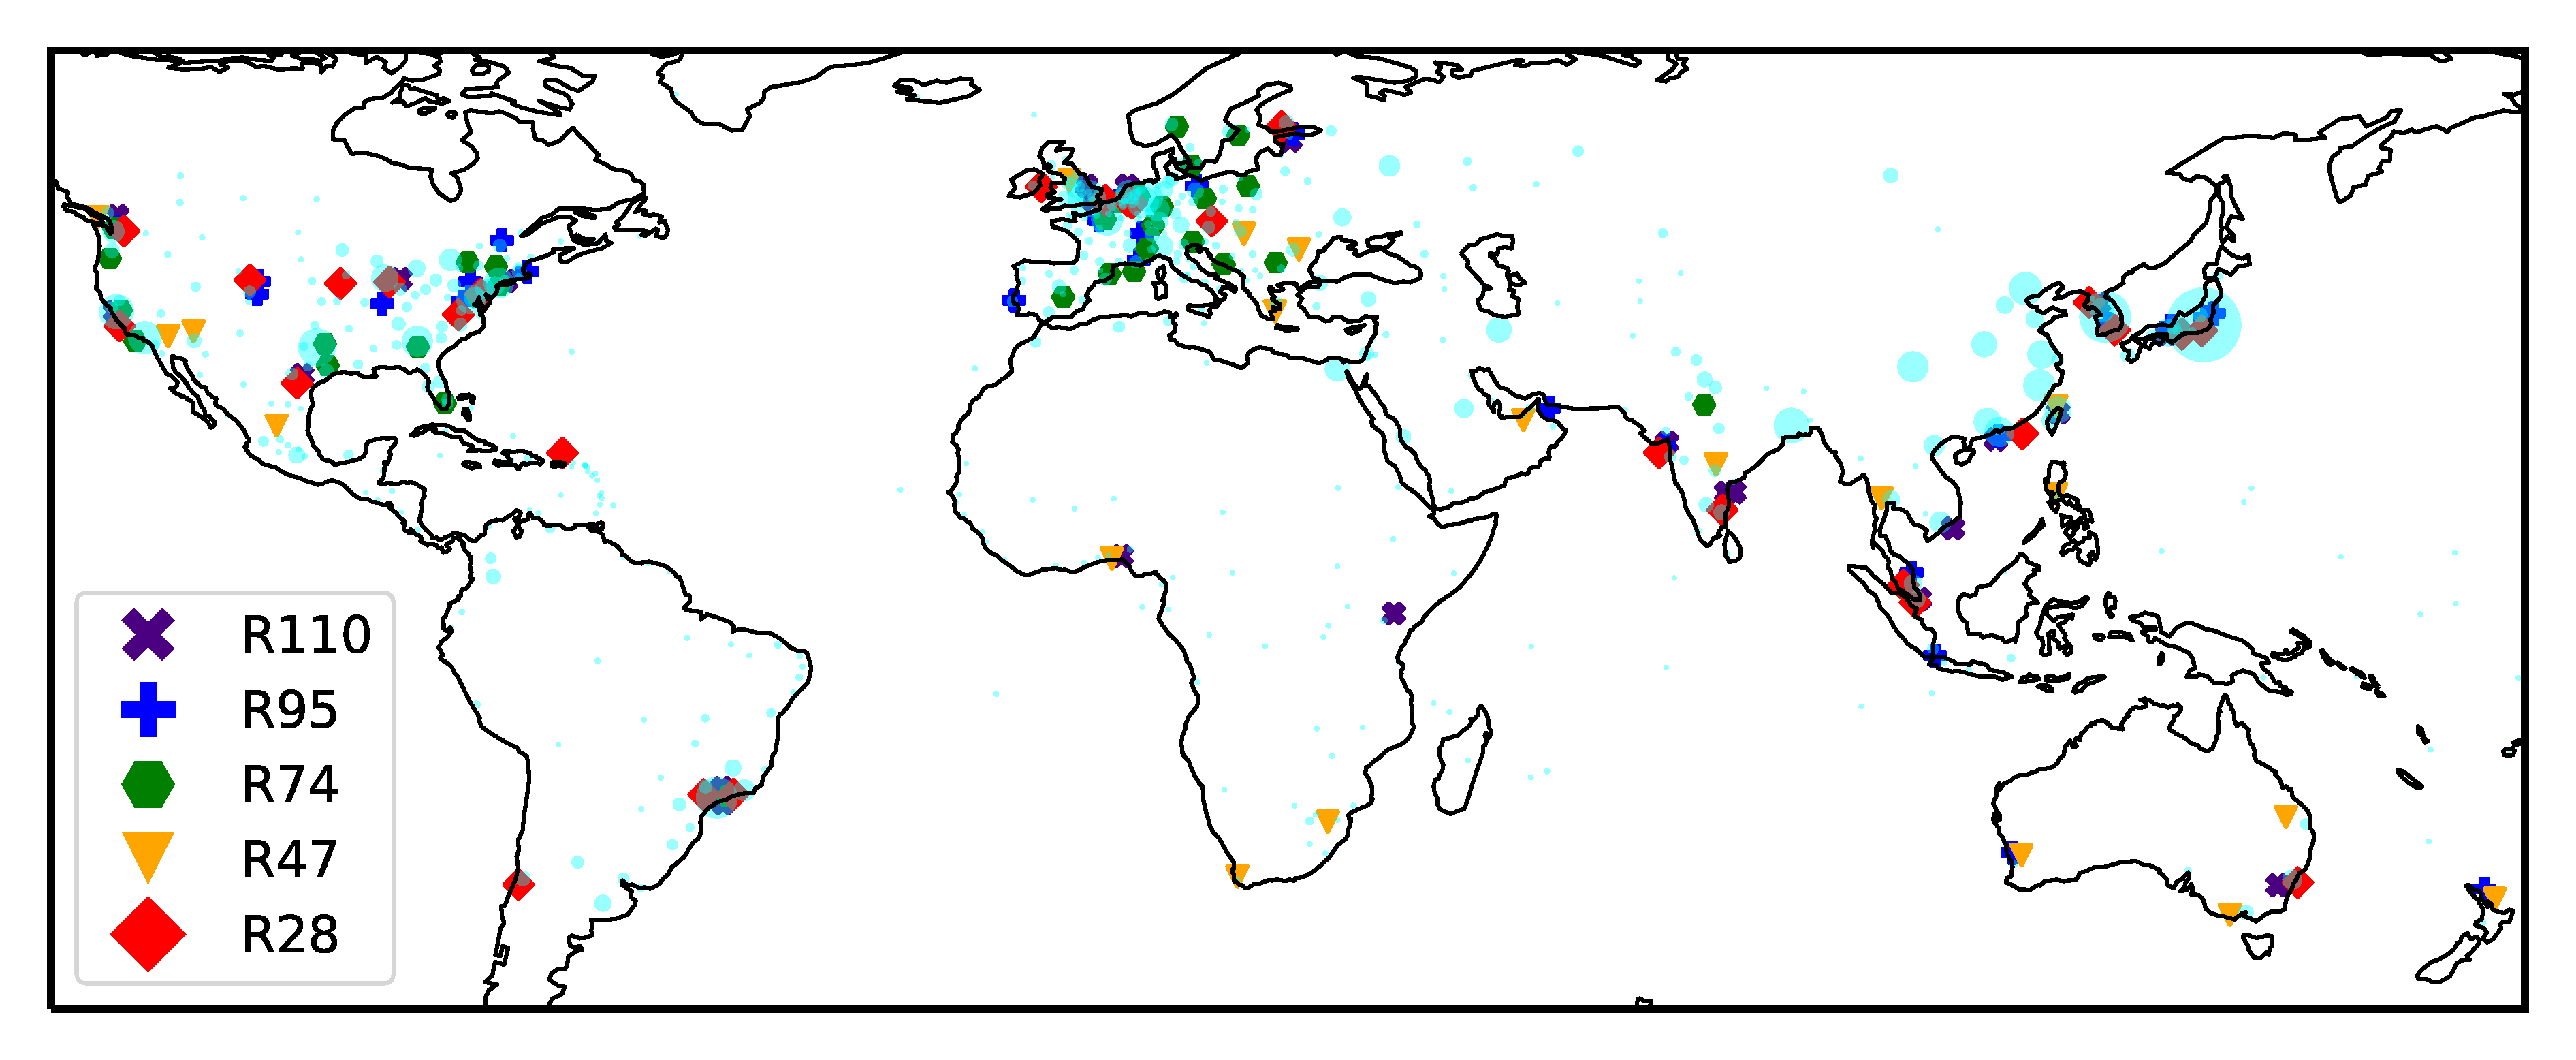
\includegraphics[width=\linewidth]{figures/microsoft_deployment_map.pdf}
    \caption{The hierarchical ring structure, and its global presence. User populations are shown as circles, with the radius of the circle proportional to the number of users in that region. The CDN has deployed \feplural in areas of high user concentration to provide low-latency options to as many users as possible.}
    \label{fig:microsoft_deployment_map}
\end{figure}

\section{Methodology and Datasets}\label{methodology-and-datasets-1}

\label{sec:methodology_datasets}

We have one dataset for each of the services using anycast we study. The
data we use to analyze the root DNS is readily available \cite{ditl},
while the CDN data is proprietary, gathered from an internal measurement
system the CDN operates . We supplement these datasets with measurements
from RIPE Atlas \cite{staff2015ripe}, a global measurement framework. As
of May 2020, RIPE Atlas has more than 11k active measurement probes in
hundreds of countries.

\subsection{Root DNS Data and
Methodology}\label{root-dns-data-and-methodology-1}

\label{sec:root_dns_data_sources}

To measure how root DNS latency impacts users, we would ideally track
root DNS queries from the moment they are triggered (e.g., during a web
page load), and determine when those DNS queries are in the `critical
path' of the process users are executing. However, with diverse
operating systems and applications, many trying to reduce user-perceived
latency, such a measurement is impossible, especially at scale. Instead,
we rely on two DNS data sets: long-term packet captures from \ISIone,
and from Day In the Life of the Internet (DITL), 48-hour packet captures
at most root servers \cite{ditl}.

To obtain a local view of root DNS queries, we use packet captures from
a recursive resolver serving users at \ISIone. The recursive resolver
runs BIND v9.11.14. The captures, from 2014 to the present, reflect all
traffic (incoming and outgoing) traversing port 53 of the recursive
resolver. We use traces from 2018, as they are relatively recent and
overlap temporally with other datasets we use. This recursive resolver
received queries from approximately 200 unique IP addresses each day
over 2018. This recursive resolver serves some general users on laptops,
and a number of desktop and rack-mounted computers of a network research
group, so the results may deviate from a typical population. We did
examine the dataset for anomalies like measurement experiments and found
none in the period we use.

To obtain a global view of root DNS use, and how these queries translate
to user latency, we use the 2018 Day in the Life of the Internet (DITL)
captures, archived by DNS-OARC \cite{ditl} (the most recent available
when we began this work). DITL occurs approximately annually, with each
event including data from most root servers. The 2018 DITL took place
2018-04-10 to -12 and included 12 root letters (all except G-Root). IP
addresses from B- and I-Root are partially or fully anonymized. Since we
only comment on qualitative results (orders of magnitude), the exclusion
of I Root and G Root traffic from analysis in
\Cref{sec:root_dns_latency} likely does not affect our high-level
conclusions. All roots except H-root group the captures by site, giving
us a global yet detailed description of what traffic is reaching various
servers throughout the world.

We pre-process this dataset to remove queries we do not believe affect
user latency. Of the 51.9 billion daily queries, we discard 31 billion
queries to non-existing domain names and 2 billion PTR queries. About
28\% of non-existing domain name queries are captive portal detection
from Google's Chromium browser \cite{broot_invalid_queries}, and so
involve machine startup and not browsing latency. We believe most of the
remainder are generated by other malfunctioning, automated software.
Similarly, while PTR queries have some uses (traceroutes and confirming
hostnames during authentication), they are not part of typical user web
latency. We explore this decision, its effects on our conclusions, and
provide further justification for this pre-processing step in
\Cref{ap:invalid_queries}.

Sources of DNS queries in the DITL captures are, almost always,
recursives, so the captures alone provide little information about how
many users use each recursive resolver, or how many DNS queries each
user makes. To estimate per-user latency, we augment these traces with
the approximate number of users of recursives, gathered in 2019. This
user data is from DNS data at a large CDN, and it counts unique IP
addresses as ``users''. We recognize this definition may undercount
multiple human users that use a single IP address with Network Address
Translation (NAT). The large CDN maps recursives to user IP addresses by
instrumenting users to request DNS records for domains the CDN controls
when users interact with the CDN, a technique described in the
literature \cite{mao2002precise, calder2018odin}.

\begin{table}[]
\centering
\resizebox{\linewidth}{!}{%
\begin{tabular}{|l|l|l|}
\hline
\textbf{Data Set}                            & \textbf{Statistic} & \textbf{Percent Overlap} \\ \hline
\multirow{4}{*}{DITL $\cap$ CDN}             & DITL Recursives          & 29.3\% of DITL Recursives                            \\ \cline{2-3} 
                                             & DITL Volume        & 72.23\% of DITL Query Volume                            \\ \cline{2-3} 
                                             & CDN Recursives           & 78.8\% of CDN Recursives                           \\ \cline{2-3} 
                                             & CDN Volume         & 88.1\% of CDN Query Volume                            \\ \hline
\multirow{4}{*}{DITL $\cap$ CDN $\cap$ RIPE} & DITL Recursives          & .14\% of DITL Recursives                              \\ \cline{2-3} 
                                             & DITL Volume        & 20.7\% of DITL Query Volume                           \\ \cline{2-3} 
                                             & CDN Recursives           & .34\% of CDN Recursives                              \\ \cline{2-3} 
                                             & CDN Volume         & 54.6\% of CDN Query Volume                            \\ \hline
\end{tabular}%
}
\caption{Statistics displaying the extent to which the recursives of users in a large CDN overlap recursives seen in the 2018 DITL captures. Also shown is the extent to which recursives of RIPE probes represent the 2018 DITL captures. For example, the percent overlap of DITL recursives in DITL $\cap$ CDN is the number of DITL recursives in DITL $\cap$ CDN divided by the number of recursives in DITL.}
\label{tab:dataset_matching_statistics}
\end{table}

We then join the DITL captures and CDN user counts by the recursive
resolver /24, aggregating the DITL query volumes from that /24 prefix
with the CDN user IP counts seen using those resolvers.\footnote{We take
  care to ensure that user counts are not ``double counted'' across
  different resolver IP addresses in the same /24.} We aggregate by /24
to increase the amount of recursives for which we have user data, noting
that organizations may use many colocated servers using the same /24 as
recursives \cite{google_public_dns, opendns_public_dns}. Prior work has
also found that up to 80\% of /24's are collocated
\cite{gharaibeh_colocation_24}. We further explore this decision,
explore its implications on our results, and provide further
justification for this pre-processing step in \Cref{ap:join_by_24}. For
clarity, we henceforth refer to these /24's as recursives, even though
each /24 may represent several recursives. We call this joined data set
of query volumes and user counts by recursive DITL\(\cap\)CDN. We next
remove queries from prefixes in private IP space \cite{private_ips} (7\%
of all queries). Finally, we analyze only IPv4 data and discard IPv6
traffic (12\% of queries) since we do not have IPv6 user data.

There is a mismatch in the recursives present in each data set.
\Cref{tab:dataset_matching_statistics} summarizes the extent to which
the CDN data (which is a subset of all users in the world) overlaps the
DITL captures, and vice versa. Although the DITL\(\cap\)CDN only
represents 29.3\% of all recursives seen in DITL, it captures a
disproportionately large amount of all DITL volume (72.2\%). However, we
acknowledge that the lack of overlap summarized in
\Cref{tab:dataset_matching_statistics} suggests the analysis we perform
may not be representative. In \Cref{ap:apnic_root_latency_per_day} we
use a different data source of user populations and methodology to
amortize DITL queries over populations and arrive at roughly the same
conclusions, lending credence to our overall conclusions about root
latency experienced by users.

\subsection{Anycast CDN Data Sources}\label{anycast-cdn-data-sources-1}

\label{sec:cdn_data_sources} To study performance in the anycast CDN, we
use two major data sources: server-side logs and client-side
measurements. Server-side logs (\ie at \feplural) collect information
about user TCP connections, including the user IP address and TCP
handshake RTT. Using these RTTs as latency measurements, we compute
median latencies from users to \feplural,\footnote{We also looked at
  other percentiles (e.g. \(95^{th}\)), and found the qualitative
  results to be similar.} by user AS, location, and serving \fe. The CDN
determines the location and AS of users using internal databases.

User locations are tracked by \emph{region}, a geographic area used
internally by the CDN to break the world into \emph{regions} that
generate similar amounts of traffic and so contain similar numbers of
users. A region often corresponds to a large metropolitan area. We often
refer to users at the \metroas granularity, because users in the same
\metroas are often routed to the same \feplural and so (generally)
experience similar latency. There are about 500 regions in total: 130 in
Europe, 60 in Africa, 100 in Asia, 1 in Antarctica, 130 in North
America, 40 in South America, and 25 in Oceania.

The client-side measurements, described briefly in
\Cref{sec:root_dns_data_sources}, come from a measurement system
operated by the CDN, similar to those described in the literature
\cite{mao2002precise, calder2018odin}. From this CDN measurement system,
we collect latencies of users populations, noting the location and AS of
the user. With this measurement system, we are able to hold the user
population constant, for a given \metroas, across rings. Holding user
populations constant enables us to remove biases in latency patterns due
to differences between enterprise and residential traffic. Since these
measurements come directly from end-users, however, we do not know which
\fe the user hit. For both client-side measurements and server-side logs
we collect statistics of millions of users across approximately 15,000
\metroas pairs.

We also use RIPE Atlas to ping rings, so we can directly compare latency
to those collected by the CDN, to provide approximate latency (latency
from the CDN is considered proprietary). In total, we collect 7,000
measurements from 1,000 RIPE probes in more than 500 ASes to augment the
CDN latency measurements.

\section{Latency Impact on End Users}\label{latency-impact-on-end-users}

\label{sec:latency_performance_difference} To understand anycast
performance, we first investigate latency for both the root DNS and
CDNs. We quantify the latency users experience, how latencies between
services compare to each other, and the effects additional sites have on
user latency.

\subsection{Impact of Root DNS Latency on
Users}\label{impact-of-root-dns-latency-on-users}

\label{sec:root_dns_latency} To assess how root DNS performance impacts
end users, we take two perspectives: local (close to the user) and
global (across millions of users). Local evaluation estimates the
fraction of page load time users wait for root DNS resolution, while
global analysis estimates the total time per day users worldwide wait
for root DNS resolution. We find that users likely spend less than 10 ms
waiting for root DNS resolution during a page load (local view), and no
more than a few tens of milliseconds per day waiting for root DNS
resolution (global view). Hence, root DNS performance matters little to
the user.

\textbf{A Local Perspective of Root DNS Latency}

We first quantify how much latency users see from root DNS latency
during a web page load. We use packet captures of the recursive resolver
at \ISIthree (\cref{sec:root_dns_data_sources}). We do not claim the
behavior at this resolver is globally typical of users, but believe we
may still draw valuable qualitative results. We first calculate the
number of queries to the root server as a fraction of user requests to
the recursive resolver. We refer to this metric as the root cache miss
rate, as it approximates how often a TLD record is not found in the
cache of the recursive in the event of a user query. We say
approximately since, for example, the recursive resolver may have sent
multiple root requests per user query, or root requests without any user
query triggering them.

\begin{table}[]
\centering
\resizebox{\linewidth}{!}{%
\begin{tabular}{lll}
                                                             &                                                                                                                           &                             \\ \hline


\multicolumn{1}{|l|}{\multirow{2}{*}{\textbf{Statistics}}}   & \multicolumn{1}{l|}{Number of User Queries (millions)}                                                                  & \multicolumn{1}{l|}{14.9}   \\ \cline{2-3} 
\multicolumn{1}{|l|}{}                                       & \multicolumn{1}{l|}{Number of Root Transactions}                                                                          & \multicolumn{1}{l|}{73,200} \\ \hline
\multicolumn{1}{|c|}{\multirow{3}{*}{\textbf{Assumptions}}}  & \multicolumn{1}{l|}{Web Page Load Time (ms)}                                                                              & \multicolumn{1}{l|}{3,000}  \\ \cline{2-3} 
\multicolumn{1}{|c|}{}                                       & \multicolumn{1}{l|}{Root DNS Latency (ms)}                                                                                & \multicolumn{1}{l|}{500}    \\ \cline{2-3} 
\multicolumn{1}{|c|}{}                                       & \multicolumn{1}{l|}{\begin{tabular}[c]{@{}l@{}}Number of DNS Look-Ups \\ Per Web Page\end{tabular}}                       & \multicolumn{1}{l|}{3}     \\ \hline
\multicolumn{1}{|l|}{\multirow{3}{*}{\textbf{Implications}}} & \multicolumn{1}{l|}{\begin{tabular}[c]{@{}l@{}}Percent of user Queries \\ Resulting in a Root Transaction\end{tabular}} & \multicolumn{1}{l|}{0.5}    \\ \cline{2-3} 
\multicolumn{1}{|l|}{}                                       & \multicolumn{1}{l|}{\begin{tabular}[c]{@{}l@{}}Expected Speed-up in PLT with \\ No Root Latency (ms)\end{tabular}}        & \multicolumn{1}{l|}{8 ms}   \\ \cline{2-3} 
\multicolumn{1}{|l|}{}                                       & \multicolumn{1}{l|}{Resulting PLT Speedup (percent)}                                                                      & \multicolumn{1}{l|}{0.25\%}   \\ \hline
\end{tabular}%
}
\caption{Root querying statistics gathered from \ISItwo recursive for a representative month of 2018, and associated implications of how root latency impacts users of ISI. }


\label{tab:isi_cache_hit_rate_stats}
\end{table}

\Cref{tab:isi_cache_hit_rate_stats} gives relevant statistics and their
implications on user-perceived latency. The daily root cache miss rates
of the resolver range from 0.1\% to 2.5\% (not shown), with a median
value of 0.5\%. The global cache miss rate across 2018 was also 0.5\%,
so we choose to include this median/global value in
\Cref{tab:isi_cache_hit_rate_stats}.

We use this root cache miss rate to approximate latency experienced by
users during a web page load. Assume that a web page load takes
\(\mathnormal{W}\) ms, that there are \(\mathnormal{S}\) serial DNS
requests per page, that the root latency is \(\mathnormal{l_r}\) ms, and
that the root cache miss rate is \(\mathnormal{m}\). Then, the resulting
(average) latency due to root DNS resolution per page load is
approximately given by \(\mathnormal{m l_r S}\),\footnote{We are
  modeling cache hits as Bernoulli trials with parameter m. Since m is
  small, the probability of two or more cache misses in S DNS requests
  is negligible.} which, as a fraction of page load time is
\(\frac{m l_r S}{W}\).

Although \(\mathnormal{W}\) and \(\mathnormal{l_r}\) depend on a number
of factors (e.g.~browser, web page size), \(\mathnormal{m}\) can be
measured for each recursive resolver (as shown in
\cref{tab:isi_cache_hit_rate_stats}), and \(\mathnormal{S}\) is usually
small. We use \(\mathnormal{S}\) = 3 as a typical value. To measure
\(\mathnormal{S}\), we perform page loads for the 1,000 most popular
domains, taken from GTmetrix \cite{gtmetrix}, using the Selenium
web-browser and calculate the number of blocking DNS requests per page
load using previously developed methods \cite{sundaresan2013web}. We
find 95\% of page loads result in \(\mathnormal{S}\) \(\leq\) 3. As
exaggerated upper bounds on the impact of root DNS latency, we choose
\(\mathnormal{W}\) = 3,000 ms (a fast page load) and
\(\mathnormal{l_r}\) = 500 ms (a slow root latency).\footnote{According
  to HTTP Archive \cite{http_archive}, RIPE Atlas \cite{staff2015ripe},
  and the results from \ISItwo, these are quite conservative estimates
  in the sense that they \emph{overestimate} root DNS latency's effect
  on PLT.}

The upper bound on how much latency a user could save, if root quieres
were free, is only 8ms \(0.005 \times 500 \times 3\)). As a percentage
of the total page load time, this latency is \(\frac{8}{3,000}\) =
0.25\%, which is measurable, but likely makes little difference to
users. For comparison, a conservative estimate of the root cache miss
rate of 2.5\% (as opposed to .5\%), would result in root DNS resolution
comprising approximately 1.25\% of a single page load
(\cref{tab:isi_cache_hit_rate_stats}). In
\Cref{ap:latency_measurements_isi} we provide another visualization of
the minimal impact root DNS latency has on users of \ISItwo, and all DNS
latency users at \ISItwo experience.

The above demonstrates the impact of root DNS latency on users is small
(a few milliseconds). However, the impact of root DNS latency on user
performance is still not as small as one would expect. For example, a
particular day during January 2018 sees as many as 900 queries to the
root server for the COM NS record. Given the 2 day TTL of this record,
900 queries per day is an unexpectedly large frequency. We explore this
issue further in \Cref{ap:redundant_queries}, and find such problems may
be caused by software bugs. This unexpectedly large number of queries
suggests arguments that users rarely experience root latency because
cached TLD records have long TTLs are not sufficient. To obtain more
accurate estimates of what root DNS latency users experience (as opposed
to what they could \emph{ideally} experience), we next take a global
view of root DNS querying behavior.

\textbf{A Global Perspective of Root DNS Latency}

Towards obtaining a global view of how users interact with the root DNS,
we look at global querying behavior of recursives. Given query volumes
towards root servers from recursives and user counts behind each
recursive from the DITL captures (\cref{sec:root_dns_data_sources}) , we
are able to estimate the amount of latency users experience per day due
to root DNS resolution. \Cref{fig:user_root_latency_per_day} is a CDF of
expected user latency per day, where the expected value is calculated
according to certain assumptions we make about root latency (we
enumerate these assumptions below). \Cref{fig:user_root_latency_per_day}
demonstrates that 50\% of users spend no more than 85 ms of latency per
day waiting for root DNS queries, regardless of which method is used to
estimate daily latency.

\begin{figure}
    \centering
    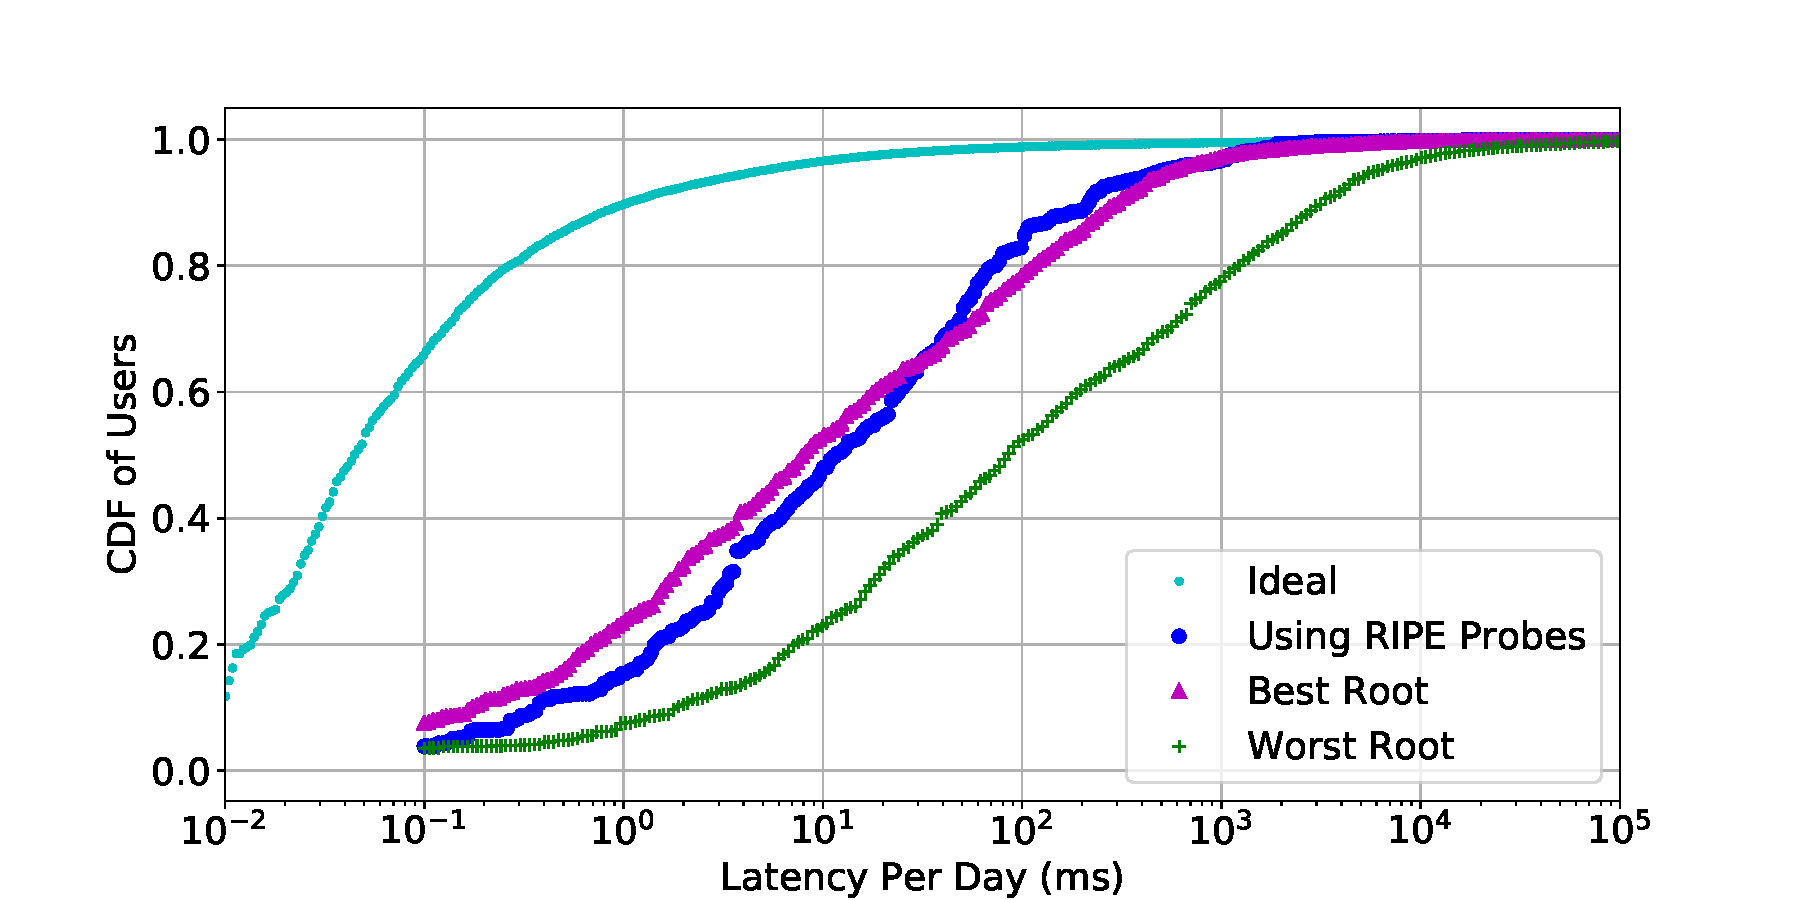
\includegraphics[width=\linewidth]{figures/user_root_latency_per_day.pdf}
    \caption{A CDF of approximate latency a user experiences due to root DNS resolution, per day, where the lines represent different ways of estimating root latency. Even using the worst (highest latency) root server, users experience no more than 85 ms per day of root latency.}
    \label{fig:user_root_latency_per_day}
\end{figure}

\begin{figure}
    \centering
    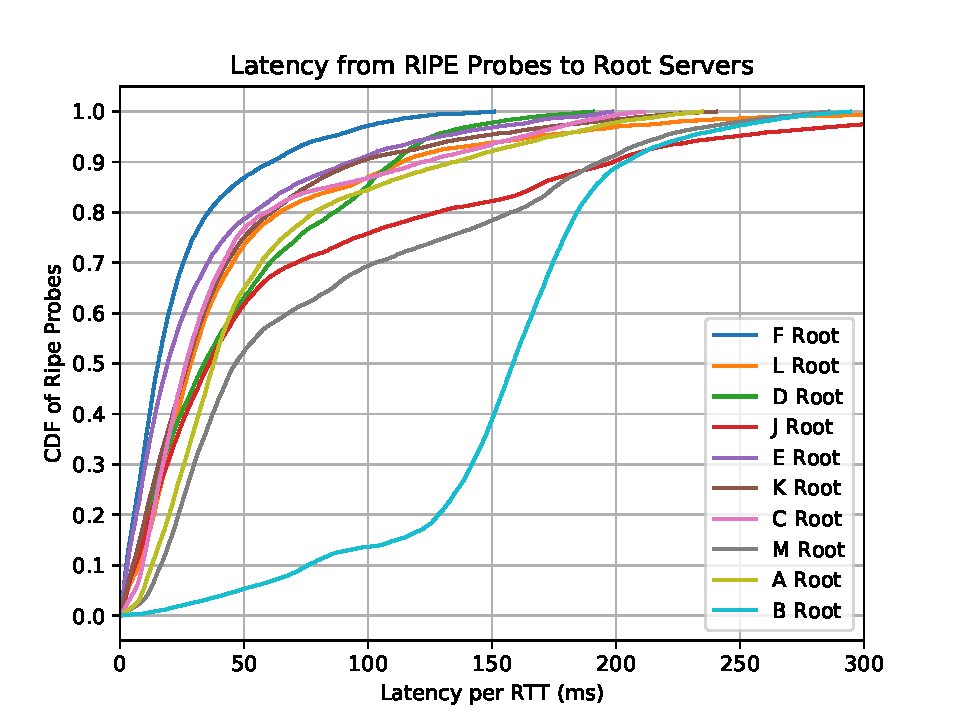
\includegraphics[width=\linewidth]{figures/ripe_root_latencies.pdf}
    \caption{Latencies from approximately 10,000 RIPE probes to root DNS servers on a day in April 2018 (the month of the DITL captures). Letters in the legend are listed in the order of deployment sizes (in April, 2018), and we also show deployment size for clarity. Larger deployments clearly lead to lower latencies, although the trend is not absolute.}
    \label{fig:ripe_root_latencies}
\end{figure}

To generate each line in \Cref{fig:user_root_latency_per_day}, we
multiply the expected root latency per query for each recursive by the
number of queries per day each recursive makes and divide by the number
of users that recursive represents. We estimate the expected root
latency per query for each recursive in a few different ways which we
describe below. This product (representing daily query latency per user)
is then weighted by user count and the resulting CDF is calculated. We
calculate the number of queries per day each recursive makes from DITL
by first calculating daily query rates at each site (\ie total queries
divided by total capture time) and subsequently summing these rates
across sites. As we include nearly every root query captured across the
root servers, \Cref{fig:user_root_latency_per_day} provides a truly
global view of how users incur latency due to the root DNS.

Since we do not know the actual latencies from recursive to each root,
we estimate expected latency in multiple ways. First, we obtain
latencies from RIPE Atlas probes to root servers during the same time as
the DITL captures. \Cref{fig:ripe_root_latencies} shows a CDF of the
median latency over the day, as reported by each of the \(\sim\) 10k
active observers.

The lines labelled ``Best Root'' and ``Worst Root'' in
\Cref{fig:user_root_latency_per_day} correspond to cases in which the
latency from every recursive to every root are 15 ms and 159 ms,
respectively. These latencies are the median (across RIPE probes)
latencies to F and B root, and are the lowest and highest such medians
(\ie ``leftmost'' and ``rightmost'') in \Cref{fig:ripe_root_latencies}.
Comparing Best Root and Worst Root demonstrates that the choice of root
server makes little difference to the user (roughly 100 ms/day at the
median), despite the ``much better'' performance of the Best Root when
looking at \Cref{fig:ripe_root_latencies} in isolation. Put another way,
the median user would only query the roots once per day (due to
caching), and so would only experience the difference between the Best
Root and Worst Root once per day.

The line labeled ``Using Ripe Probes'' looks only at those recursives in
the DITL\(\cap\)CDN data set who are recursives for RIPE probes. We
obtained the recursive resolver for approximately 3,000 RIPE probes from
collaborators. Our collaborators used 3,000 RIPE Atlas probes (a random
subset of RIPE probes are available to execute measurements at any given
time) to query DNS records hosted by a server they control and joined
logs by the unique DNS record they allotted to each RIPE probe
\cite{lucas_ripe_potential}. From
\Cref{tab:dataset_matching_statistics}, we see that /24's housing
recursives of the above mentioned 3,000 RIPE probes only account for
21\% of the volume in DITL and about 0.1\% of all /24's; hence, RIPE
probes are a small part of the population (as expected). However, for
users using these recursives to resolve DNS queries, the `Using RIPE
probes' line could be a fairly accurate measurement of the expected
daily latency due to root DNS resolution. Additionally, studies use RIPE
probes when measuring anycast latency so this line could provide a
useful comparison to prior work
\cite{colitti2006evaluating, de2017anycast, li_levin_spring_bhattacharjee_2018, mcquistin2019taming}.
This method provides a low median estimate of 12 ms/day.

Finally, the line labeled `ideal' does not use DITL query volumes to
calculate daily user latency, but instead represents a hypothetical
scenario in which each recursive queries for all TLD records exactly
once per TTL, and amortizes these queries uniformly over their
respective user populations. For the ideal line, we assume latencies
from all recursives to all sites are 15 ms (Best Root, for comparison).
The resulting hypothetical median daily latency of 0.044 ms could
represent a future in which caching works at recursives optimally -- not
querying the roots when not necessary. The `ideal' line also
demonstrates the degree to which the assumption that recursives should
only query once per TTL \emph{underestimates} the latency users
experience due to the root DNS.

Since \Cref{fig:user_root_latency_per_day} presents daily latencies for
each user, it is interesting to put daily latency into perspective.
Loading a web page takes roughly 3 seconds on desktop and 7 seconds on a
mobile device \cite{http_archive}. Hootsuite, a social media management
platform, estimates users spend more than six hours per day on the
Internet \cite{hootsuite_daily_internet}, and another study at USC found
American households spend at least three hours per day on the web
\cite{digital_future}. Similarweb \cite{similarweb}, which tracks usage
of various social media services on the web, found Youtube users watch
for more than 30 minutes per day on average \cite{similarweb}. Each
method of measuring such high-level Internet usage statistics has its
drawbacks, but, clearly, latencies in
\Cref{fig:user_root_latency_per_day} are dwarfed by these statistics.
Hence, root DNS latency has little impact on user experience.

The comparison between the Worst Root and Best Root lines in
\Cref{fig:user_root_latency_per_day} reveals an important fact --
reductions in root DNS latency \emph{do not matter} for users.
Specifically, a hypothetical ten-fold decrease in latency (\ie due to
investment in new sites around the globe) provides minimal latency
savings, on the order of tens of milliseconds per day, to users. Hence,
not only does root DNS latency not affect users, but also the recent
large increase in the number of root DNS sites has likely not been
motivated by latency improvement.

\iffalse
Other things we could discuss here 1. Specifically enumerating the ways
in which the above are over-estimations of daily root DNS latency/root
latency per PLT 2. Where ISI/Columbia fit into daily user latency 3.
U.S. cell providers, and how they lie at the tail end of the curve as
expected \fi

\subsection{Impact of CDN Latency on
Users}\label{impact-of-cdn-latency-on-users}

\label{sec:anycast_cdn_latency}

We now measure how users are impacted by latency of a large anycast CDN.
Using both client-side measurements and server-side logs, we conclude
that anycast latency results in orders of magnitude more visible delay
to users for page loads from a CDN than users see due to the root DNS.
Consequently, investments in more anycast sites positively affect user
experience much more in the case of the anycast CDN.

As discussed in \Cref{sec:bg_cdn_anycast}, the anycast CDN we study has
\emph{rings} that form a logical hierarchy of layers. Each larger ring
adds some sites to those of the smaller ring. Since each ring provides
an independent IP anycast CDN service, we report results for each of the
rings individually. Rings all use split TCP connections and rely on
cloud services for content. As a result, different ring sizes reflect
some of the benefit of additional anycast locations, but we caution that
they do not reflect all the performance benefits of independent sites.\\
Users experience latency from the CDN as they retrieve web objects
(e.g.~web pages or supporting data) hosted by the CDN. Hence, in order
to assess how users of the CDN experience latency, we must measure not
only what the RTT is from users to \feplural, but also how many RTTs are
incurred when fetching a web object.

\begin{figure*}
  \centering
    \subfloat[]{
        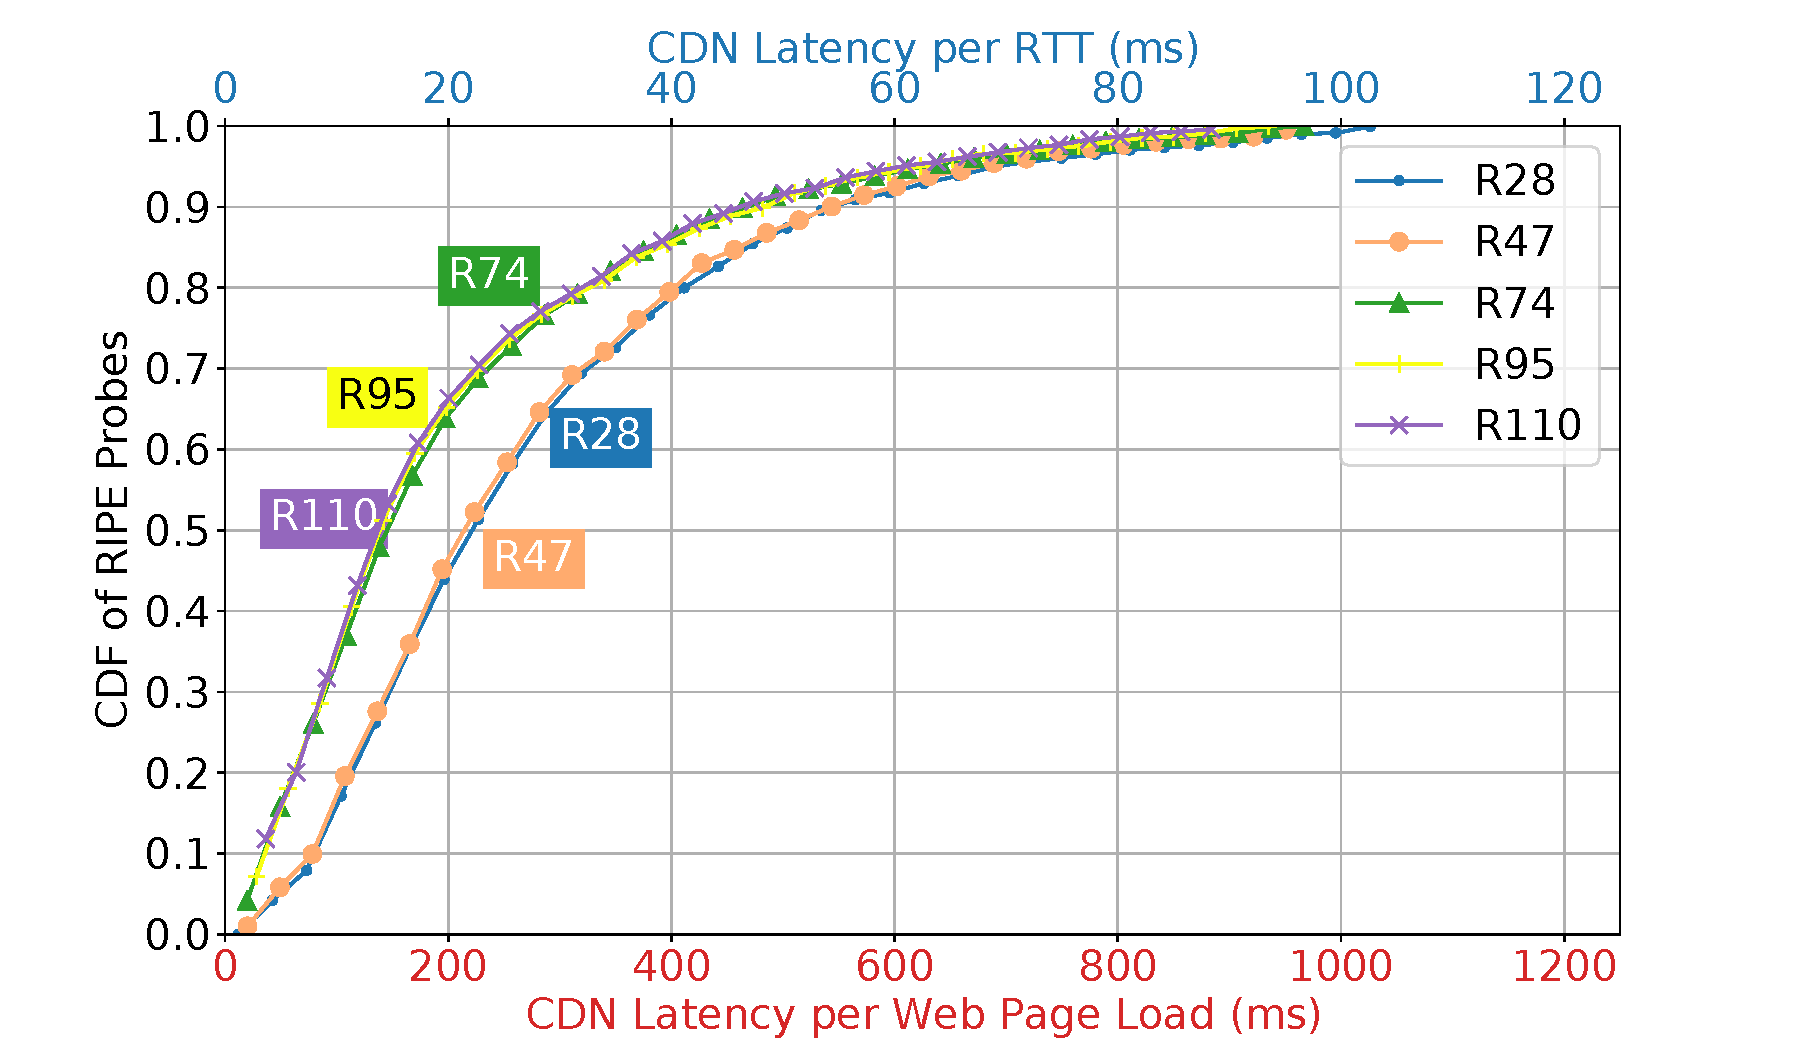
\includegraphics[width=0.33\linewidth]{figures/latency_microsoft_root-a.pdf}
        \label{fig:latency_microsoft_root-a}
    }
    \subfloat[]{
        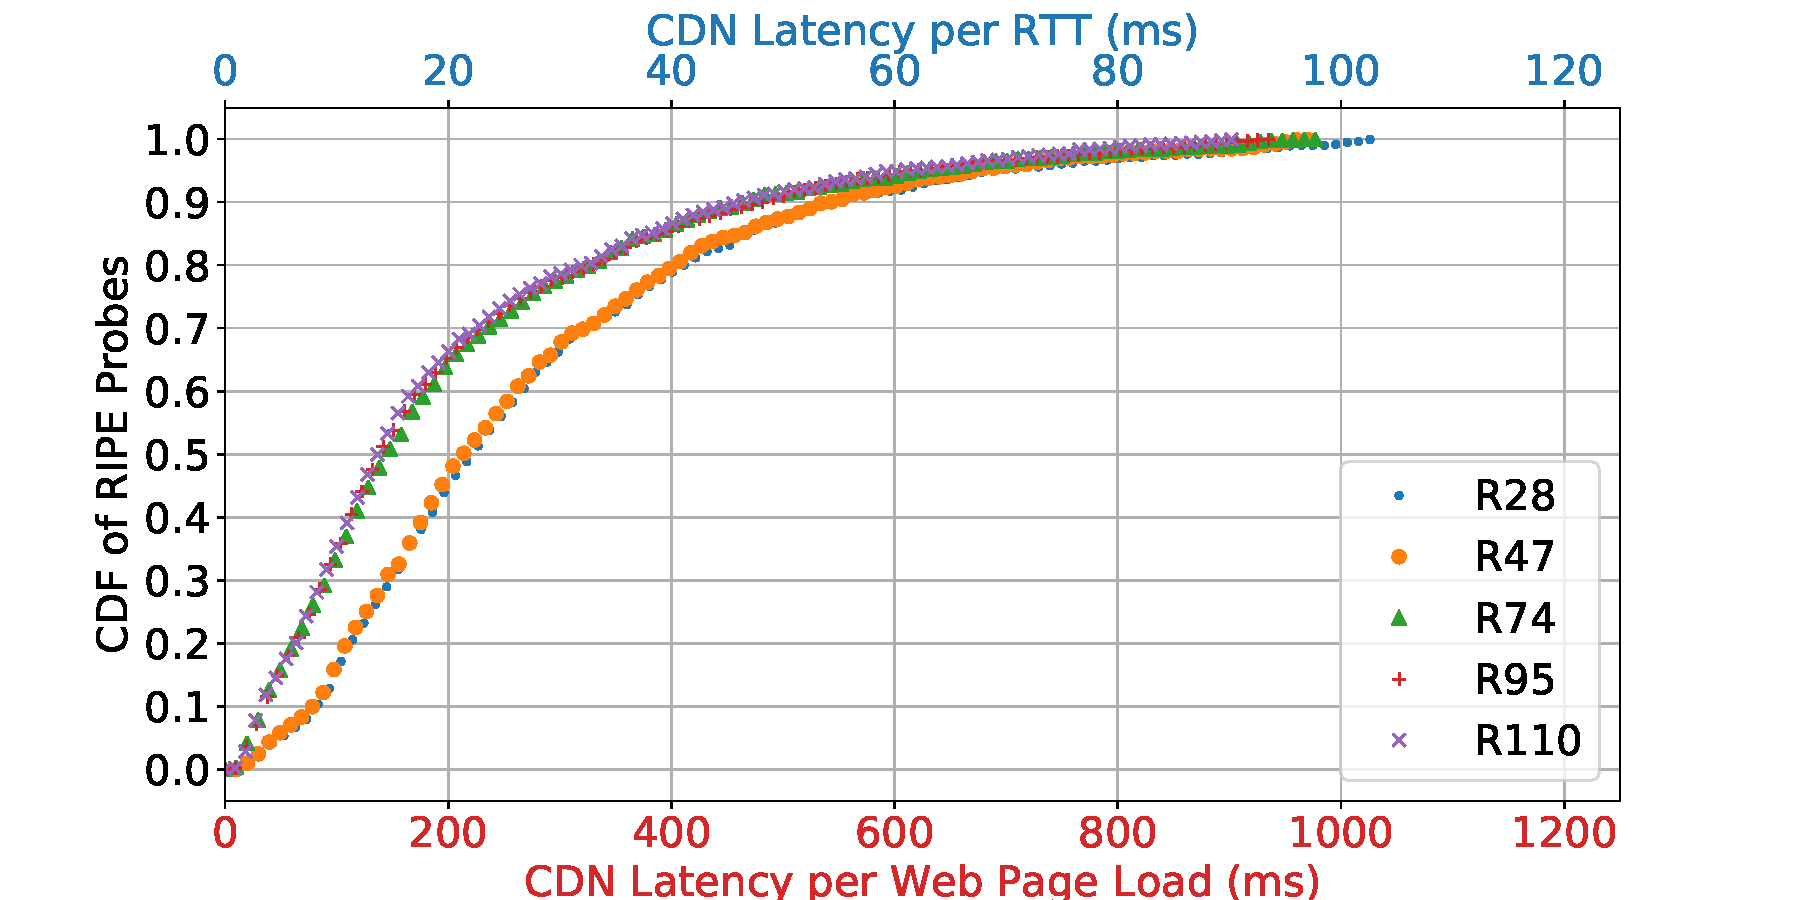
\includegraphics[width=0.33\linewidth]{figures/latency_microsoft_root-b.pdf}
        \label{fig:latency_microsoft_root-b}
    }
    \subfloat[]{
        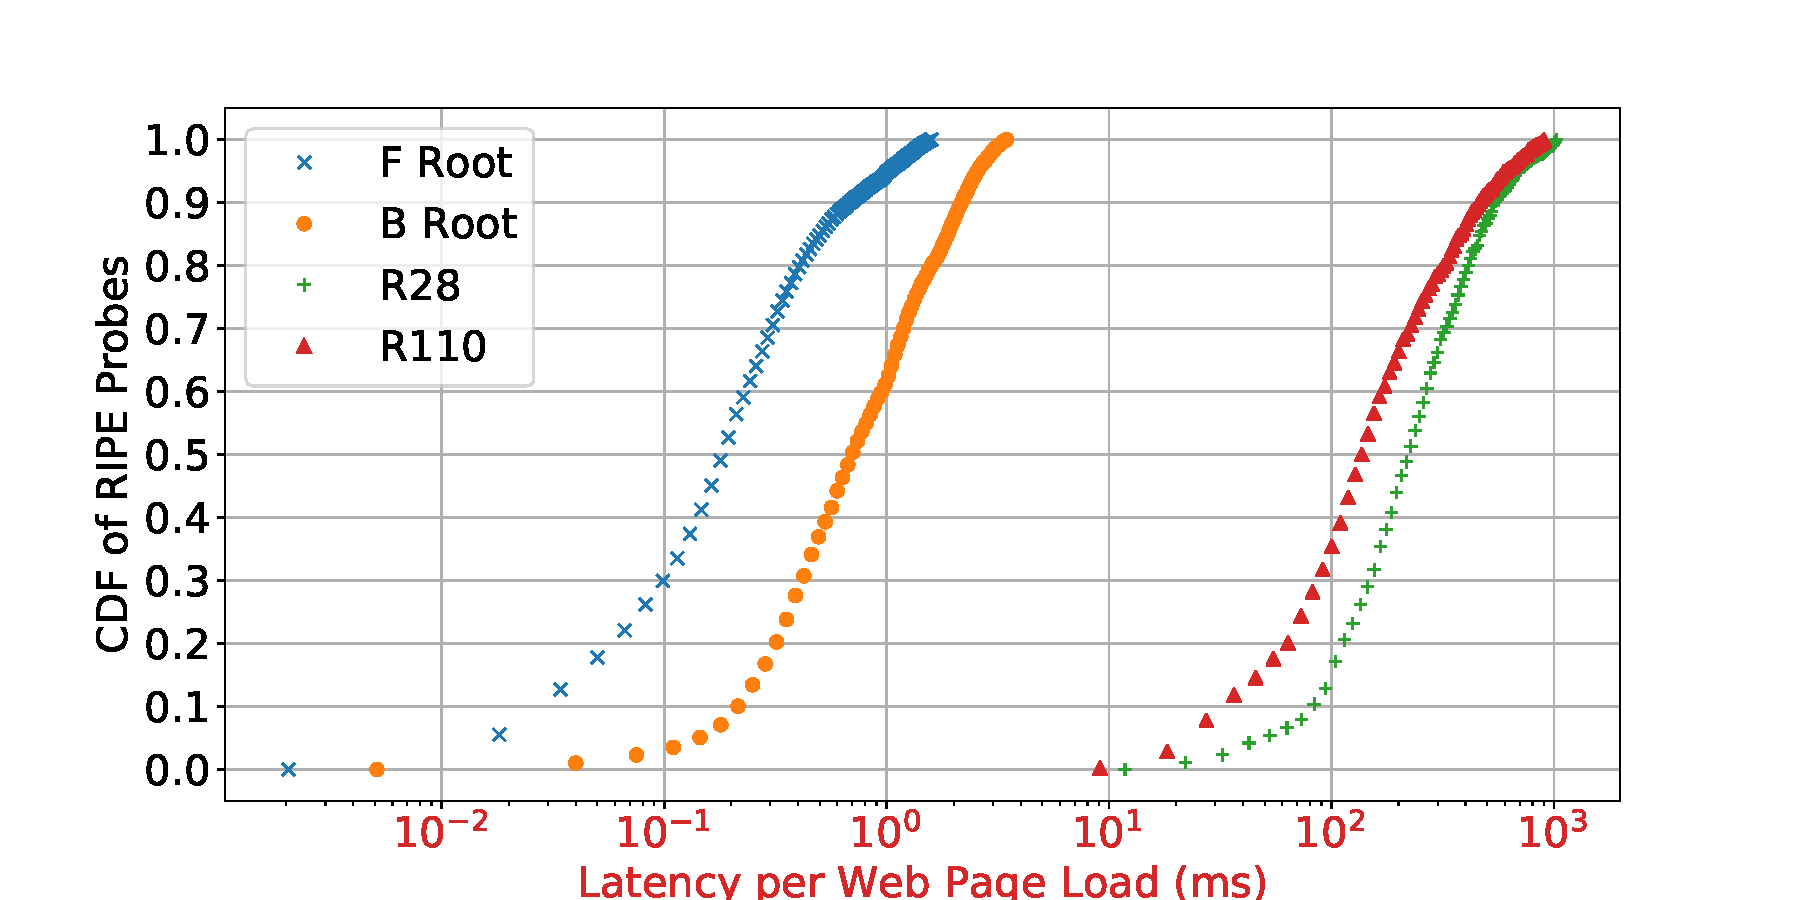
\includegraphics[width=0.33\linewidth]{figures/latency_microsoft_root-c.pdf}
        \label{fig:latency_microsoft_root-c}
    }
  
  \caption{RTTs from users to rings as measured by clients (\ref{fig:latency_microsoft_root-a}), RTTs/latencies per web page load from RIPE probes to rings (\ref{fig:latency_microsoft_root-b}), and latencies per page load are shown for B root, F root, and R118 on a log scale. Axes with per-RTT latencies are colored blue, while axes with per-page-load latencies are colored red. CDN incurred latency is orders of magnitude higher than root DNS latency (\ref{fig:latency_microsoft_root-c}).}


    \label{fig:latency_microsoft_root}
\end{figure*}

In \Cref{fig:latency_microsoft_root-a}, we show latencies from
\metroas locations to rings. We use client-side measurements in
\Cref{fig:latency_microsoft_root}, as they enable us to fix the set of
users for a given \metroas pair (see \cref{sec:cdn_data_sources}). We
show relative latencies for confidentiality reasons. Median latency
jumps significantly per RTT (5 ms) going from R47 to R74, but we see
minimal changes (2 ms at the median) in global latency for larger rings.
These changes in median latency are due to the way in which the
\feplural ``cover'' users of the CDN, a notion that we explore in
\Cref{fig:microsoft_latency_benefit_increasing_ring}.

\Cref{fig:latency_microsoft_root-b} demonstrates how RTT latency
translates into user-perceived latency in a web page load, for RIPE
probes. We use latencies from RIPE probes to quantify user-perceived
latency, since we can not share absolute latencies from CDN
measurements. Latencies per page load are calculated by multiplying
median latencies by the number of RTTs per page load (as in
\cref{sec:root_dns_latency}); for reference, we also include RTT
latencies on the top axis. The number of RTTs per page load depends on
the size of the page requested and the server's TCP implementation. We
estimate RTTs per page based on the top-1000 pages according to GTMetrix
\cite{gtmetrix} and web pages hosted by the anycast CDN, taking an
estimateof RTTs required to retrieve web page data. We find it usually
takes at least 10 RTTs to load a web page, and so use this number in
what follows. We describe these measurements and the calculation of RTTs
from page sizes in further detail in \Cref{ap:num_rtts_ppl}.

\Cref{fig:latency_microsoft_root-b} shows users can experience up to
1,000 ms in latency per page load. For large deployments (e.g.~R95),
half of RIPE probes experience approximately 100 ms of latency per page
load. We observed RIPE probes experience lower latencies to this CDN
than users do globally (not shown in figure), so
\Cref{fig:latency_microsoft_root-b} likely underestimates the latency
users typically experience. Therefore, latency to this CDN therefore
clearly factors into user experience.

The difference in median latency per page load experienced by RIPE
probes between R28 and R110 is approximately 100 ms, which is a measure
of how investments in more \feplural can help users. Although a page
load latency reduction of 100 ms may sound inconsequential, prior work
has demonstrated that higher latencies can lead to major reductions in
numbers of searches \cite{brutlag2009speed} (and therefore profits). In
addition, \emph{tail latency} has a strong effect on user retention. We
show larger rings help tail latency, moving it from about 1,000 ms to
800 ms (\cref{fig:latency_microsoft_root-b}).

\Cref{fig:latency_microsoft_root} also shows that the incremental
performance improvements from more \feplural slow as ring size
increases. To explain why these improvements slow, we show changes in
(expected) median latency for \metroas pairs when transitioning to
larger rings along with corresponding increases in population
``coverage'' in \Cref{fig:microsoft_latency_benefit_increasing_ring}.
Expectation is taken over \feplural with respect to the number of users
reaching each \fe, as is done repeatedly throughout the paper.

\Cref{fig:microsoft_latency_benefit_increasing_ring-a} shows most
\metroas pairs experience either equal or better latency to the next
largest ring with diminishing returns as more \feplural are added,
although a small fraction of users see small increases in latency when
moving to larger rings. Since
\Cref{fig:microsoft_latency_benefit_increasing_ring-a} uses client-side
measurements, we do not know why latencies change when moving from ring
to ring, since we do not know which \feplural clients use. However,
server-side logs allow an educated guess. For example, R74 has a \fe in
Atlanta, Georgia while R47 does not. Server-side logs show some users in
San Antonio get directed to Atlanta when querying R74, missing the
nearby \feplural in Texas.

Performance changes are highly correlated with the population
``coverage'' -- the fraction of users that are ``close enough'' to a
site in a ring. To demonstrate this trend, in
\Cref{fig:microsoft_latency_benefit_increasing_ring-b} we plot coverage
of each ring as a function of coverage radius. We say a \fe covers a set
of users in a \metroas pair with respect to radius \(\mathnormal{r}\) if
the \fe is within \(\mathnormal{r}\) km of the mean location of those
users. The intuition is that if a \fe is closer to a set of users, it is
likely to offer a low latency option to those users. The latency
benefits from transitioning rings correspond well to the increases in
population coverage, with the transition from R47 to R74 providing both
a large reduction in latency and larger coverage of user population. For
example, R74 has a \fe in Madrid, Spain while R47 does not. Users in all
regions and ASes of Spain are, at least in part, directed to this
\fe when querying R74. However, in R47, users in Spain usually land at a
\fe in the United Kingdom. This analysis also provides insight into why
diminishing returns are seen as more \feplural are added -- eventually,
almost all user population is covered.

\begin{figure}[]
    \centering
    \subfloat[]{
        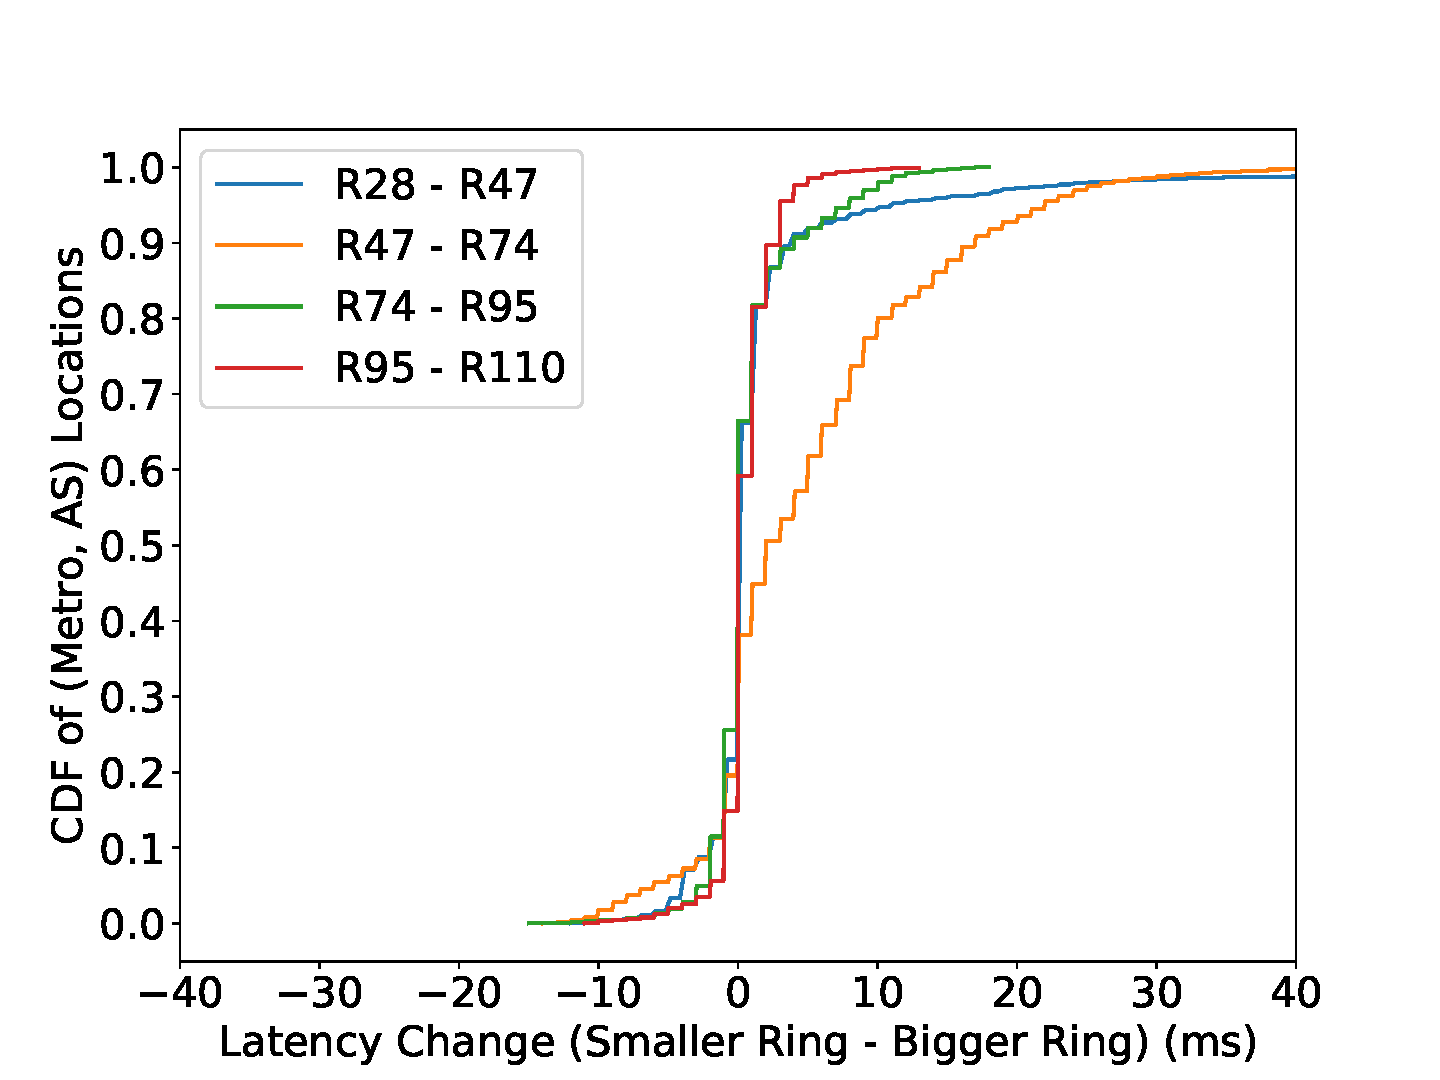
\includegraphics[width=\linewidth]{figures/microsoft_latency_benefit_increasing_ring-a.pdf}
        \label{fig:microsoft_latency_benefit_increasing_ring-a}
    } \\
    \subfloat[]{
        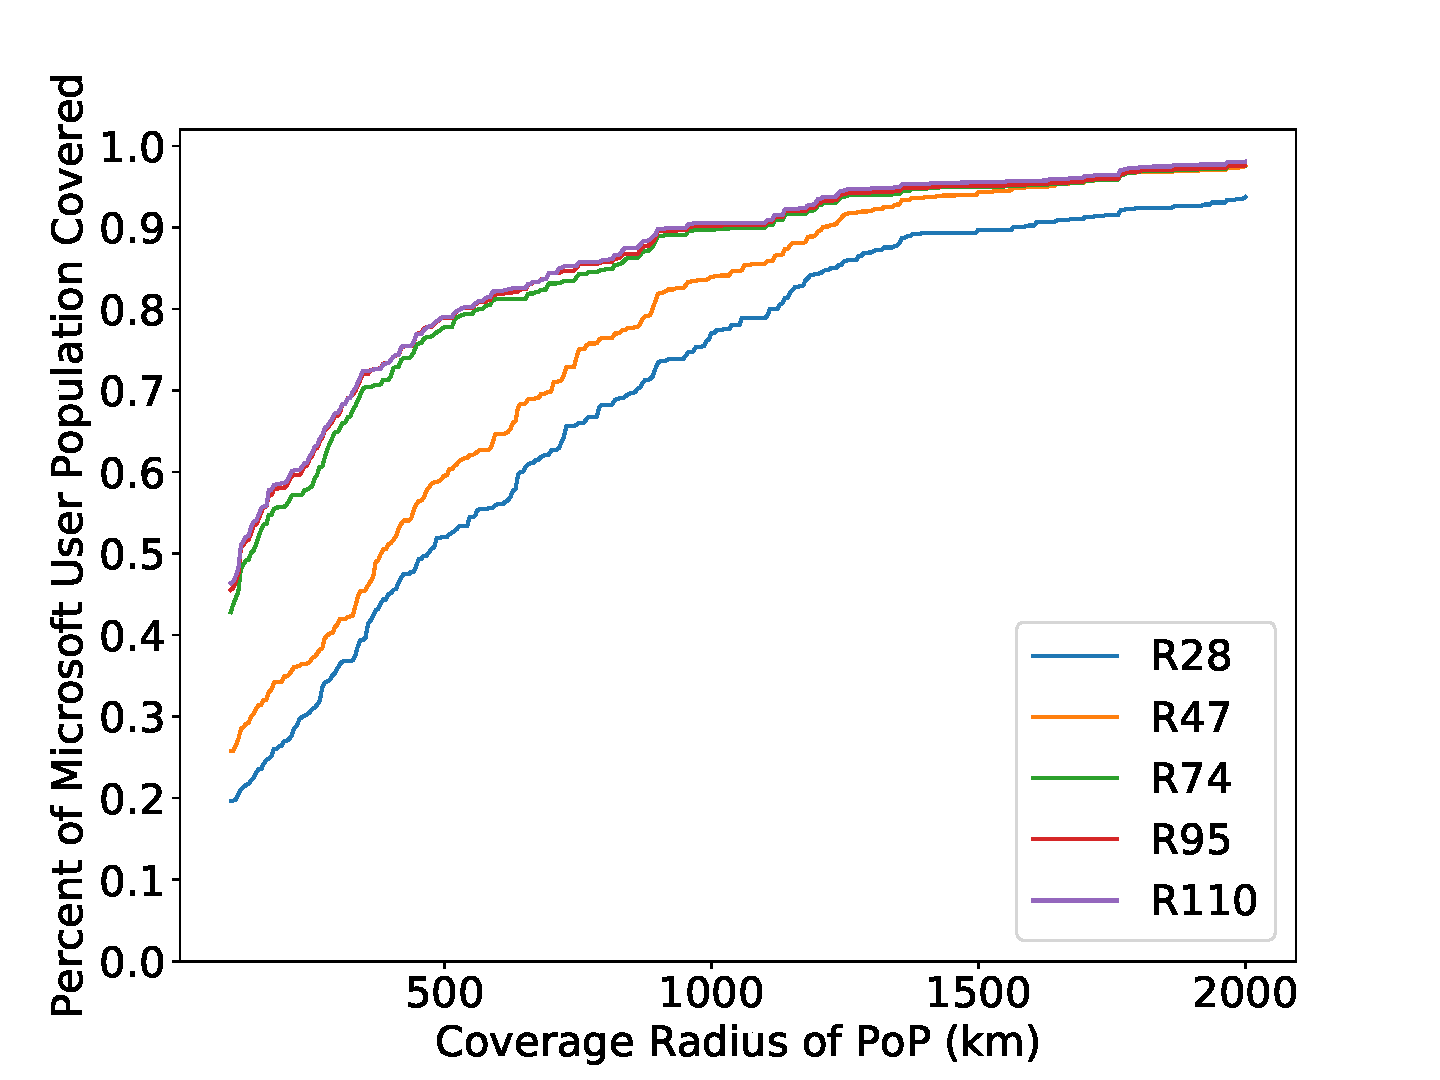
\includegraphics[width=\linewidth]{figures/microsoft_latency_benefit_increasing_ring-b.pdf}
        \label{fig:microsoft_latency_benefit_increasing_ring-b}
    }
     \caption{The change in median latency for \metroas pairs when transitioning rings (\ref{fig:microsoft_latency_benefit_increasing_ring-a}) and the corresponding increasing in population "coverage" of the anycast CDN deployment when adding front ends (\ref{fig:microsoft_latency_benefit_increasing_ring-b}). Performance generally improves for most \metroas pairs when adding more \feplural and the magnitude of the improvement corresponds to how close users are to \feplural.}
     \label{fig:microsoft_latency_benefit_increasing_ring}
\end{figure}

\subsection{Comparison}\label{comparison-2}

\label{sec:performance_comparison} To compare CDNs with root latency, in
\Cref{fig:latency_microsoft_root-c} we include per page load latencies
for F root, B root, R28 and R110. We chose these two root deployments as
they provided the best and worst median latency for RIPE probes (see
\cref{fig:ripe_root_latencies}), respectively. Clearly CDN latencies
matter \emph{orders of magnitude} more than root DNS latencies, no
matter which percentile of which curve we look at in
\Cref{fig:latency_microsoft_root-c}. Additionally, the benefit from
using a larger root DNS deployment (F root vs B root) amounts to
fractions of a ms per page load, while for the CDN using a larger
deployment (R28 vs R110) can make a difference of hundreds of
milliseconds per page load.

Looking at the \(10^{th}\) and \(90^{th}\) percentiles of each curve in
\Cref{fig:latency_microsoft_root-c}, we see that the latency penalty for
(relative) poor performance among RIPE probes is much greater for users
of the anycast CDN. For example, different RIPE probes can experience up
to a 200 ms discrepancy in per page load latency when accessing the CDN,
while probes only see at most a few ms discrepancy when accessing F
root. Since the difference between \(10^{th}\) and \(90^{th}\)
percentiles is a measure of the potential return on investment in
\fe placement, investments in new anycast sites provide orders of
magnitude more benefit for users of the anycast CDN than they do in the
root DNS.

\Cref{fig:latency_microsoft_root} is a simple, effective way of
demonstrating how users experience latency from the CDN, how much CDN
latency ``matters'', and how much more it matters to users than root DNS
latency. Although the specific quantitative impacts for users may vary
by region, AS, operating system, web page, \etc, our qualitative
observation that CDN latency matters for users, and that it matters a
lot more than root DNS latency, is likely insensitive to these
variables.

\section{Comparing Path Inflation}\label{comparing-path-inflation}

\label{sec:anycast_performance_difference} Having compared latency
between the root DNS and an anycast CDN, we now investigate anycast path
inflation in each application. As discussed in
\Cref{sec:bg_potential_drawbacks}, anycast may direct users to distant
nodes, potentially inflating latencies for users relative to the
geographic optimal. In the following we analyze how this inefficiency
manifests itself in two different anycasted services, how this
inefficiency affects users, and comparisons we can make between root DNS
and anycast CDN inefficiency.

Using the DITL captures, we find anycast path inflation in the root DNS
can send users to far-away anycast sites, unnecessarily inflating
latencies. While this inflation shows latency is not optimal, this
inflation \emph{hardly matters} to users, because caching makes queries
rare. Conversely, as few as 20\% of users of the anycast CDN experience
any path inflation, and users experience much less path inflation per
RTT than in the root DNS. The CDN's low inflation suggests it is
possible to limit anycast path inflation, and the CDN works hard to
control it given the pain it can cause to users.

\subsection{Path Inflation in the Root
DNS}\label{path-inflation-in-the-root-dns}

\label{sec:root_dns_anycast}

To measure anycast inflation for the root DNS, we look at how users are
directed to sites. The DITL captures are a rich source of data for this
purpose because they provide us with a global view of which recursives
access which locations for all but a small subset of root DNS sites.
Notably excluded from the analysis in this subsection are H root, G root
and I root, which did not provide non anonymized packet traces at the
per-site level.\footnote{Anonymization prevents us from seeing where
  queries originate.}

As discussed in \Cref{sec:bg_potential_drawbacks}, anycast path
inflation is the difference in achieved latency to an anycasted IP and
unicast path inflation. Unfortunately, calculating unicast path
inflation requires knowledge of the best unicast alternative from every
recursive seen in DITL to every root letter, something that would be
difficult to measure because some letters do not publish their unicast
addresses, and measuring from many vantage points (e.g.~RIPE probes) to
all sites would stress measurement budgets and rate limits. However,
setting unicast path inflation to 0 provides us with an
\emph{upper bound} on anycast path inflation. Therefore, using achieved
latency as an approximation for anycast path inflation suffices, since
we ultimately demonstrate anycast path inflation's effect on users is
quite small.

\begin{figure}
    \centering
    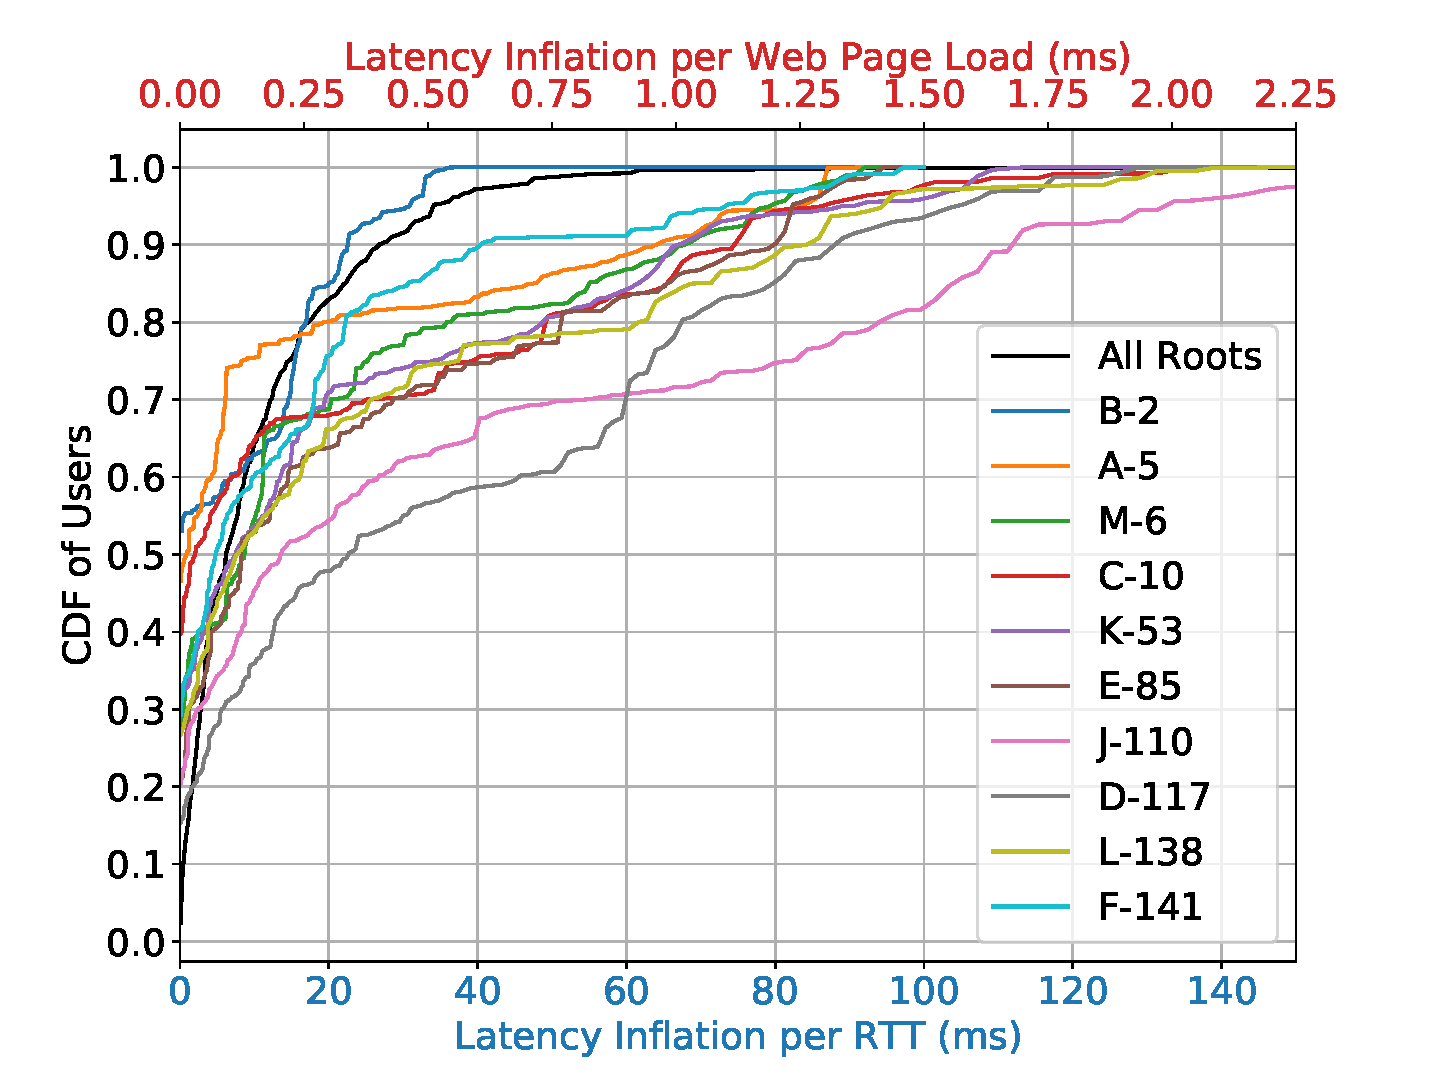
\includegraphics[width=\linewidth]{figures/API_per_RTT_PL_all_letters.pdf}
    \caption{A CDF of latency inflation per RTT (bottom axis) and per page load (top axis) for root deployments, and globally across all roots, experienced by users of a large CDN. Root letters in the legend are listed according to their deployment sizes during the DITL captures, from smallest to largest. Generally, larger deployments are likely to inflate queries. The difference between the best and worst inflation per page load is only about 2 ms in the tail. }
    \label{fig:api_per_rtt_roots}
\end{figure}

\Cref{fig:api_per_rtt_roots} shows a CDF of expected inflation per RTT
(bottom axis) and per page load (top axis) for users in the
DITL\(\cap\)CDN data set for each letter individually, and globally
(across all letters). Each point in \Cref{fig:api_per_rtt_roots} uses
the following calculation. First we geolocate all recursives in the
DITL\(\cap\)CDN data set using MaxMind \cite{maxmind}, matching prior
methodology \cite{li_levin_spring_bhattacharjee_2018}. Major public DNS
servers make server subnets and geographic locations publicly available;
\cite{google_public_dns}, allowing us to geolocate 0.4\% of (valid TLD)
DITL query volume in 2018.

We then compute anycast path inflation for each recursive sending
queries to root server \(\mathnormal{j}\) as

\begin{equation}
\label{eq:root_dns_path_inflation}
API_{j}(R) = \frac{2}{c_f} (\sum_{i_{j}} \frac{n_q(i_j) d(R, s_{i_{j}})}{N_j} -  \underset{{i_j}} {\text{min}} \; d(R, s_{i_{j}}))
\end{equation}

where \(n_q(i_j)\) is the number of queries to site \(\mathnormal{i}\)
by recursive R, \(N_j\) is the total number of queries to all sites
\(s_{i_{j}}\) in root j by recursive R, \(\mathnormal{c_f}\) is the
speed of light in fiber, the factor of 2 accounts for the round trip
latency, \(d(R, s_{i_{j}})\) is the distance between the recursive
resolver and site \(s_{i_{j}}\), and both the summation and minimization
are over the sites in this letter deployment. \(API_{j} (R)\) is
therefore an approximation of the expected latency one would expect to
see when executing a single query to root deployment j from recursive R,
averaged over all sites. The overall latency inflation of an recursive
is then the empirical mean over all roots

\begin{equation}
API^g_{root}(R) = \sum_{j} API_{j}(R) N_j / N
\end{equation}

where N is the total number of queries sent by this recursive. Each
recursive is weighted according to the number of (CDN) users behind it,
so \Cref{fig:api_per_rtt_roots} represents the latency inflation a
random user would experience when querying the roots.

It is well known that packets can take circuitous routes and so do not
travel great-circle distances to destinations. For example, prior work
suggests packets rarely effectively travel faster than \(\frac{2}{3}\)
the speed of light in fiber (\(\frac{4}{9}\) the speed of light)
\cite{katz2006towards}, when comparing great-circle distance and
measured latency. Hence, our dividing great-circle distance by
\(\mathnormal{c_f}\) is a simplification. However, using other constants
besides \(\mathnormal{c_f}\) does not change our qualitative conclusions
about inflation.

\Cref{fig:api_per_rtt_roots} demonstrates the likelihood of a root DNS
query experiencing any anycast path inflation (y-axis intercept) roughly
grows with deployment size, with a few exceptions. We also find 95\% of
users experience no more than 40 ms of latency due to inflation when
they query the roots. These findings corroborate results presented in
prior work \cite{li_levin_spring_bhattacharjee_2018} that increasing
deployment size makes inflation more prevalent.

However, we recommend placing path inflation in the perspective in two
ways. First, we consider how much actual latency it adds, not just the
percentage increase over optimal. Second, we consider all roots and not
just inflation from a few specific RIPE Atlas probes to two root
letters. As an \emph{absolute cost}, path inflation is almost always
under 10 ms for most deployments and most users. Our approximation of
anycast path inflation as total inflation is a particularly egregious
over-estimation for C root, queries to which are known to exhibit very
little anycast path inflation but quite a lot of unicast path inflation
\cite{li_levin_spring_bhattacharjee_2018}. What is perhaps most
interesting is that, although users querying any root (line `All Roots')
are quite likely to see non-zero inflation, they see less inflation in
the tail than all roots except B root.

As a useful visualization, we also display anycast path inflation
\emph{per page load} caused by root DNS queries on the top axis of
\Cref{fig:api_per_rtt_roots}. For this rescaling, we multiply latency
inflation per RTT to the root servers by the average number of RTTs to
the root servers incurred per page load, the latter of which we denote
by \(f_r\). For consistency, we approximate \(f_r\) using the statistics
found in \Cref{sec:root_dns_latency}, as 0.015 (the root cache miss rate
of 0.5\% times the number of blocking DNS requests per web page). The
top axis therefore demonstrates that this inefficiency of anycast does
not affect users in any perceptible way. Users querying the root
experience less than a millisecond of path inflation per page load, and
the difference between the most path inflation (J root) and the least
path inflation (B root) is only a couple milliseconds in the tail of
per-page-load times.

Looking at \Cref{fig:api_per_rtt_roots}, one may conclude B root is the
most ``efficient'' deployment, directing users to their closest site
most of the time. However, \Cref{fig:ripe_root_latencies} shows that
this efficiency comes because B-Root latency is higher than other
letters at the time. This latency is in part because B-Root at the time
had only sites in the Americas, and a majority of RIPE measurements are
from Europe \cite{staff2015ripe}. In early 2020 B-Root deployed three
new anycast sites, including sites in Singapore and Amsterdam, in part
to reduce latency to these regions \cite{BRoot20a}. We hope to redo our
numbers with 2020 DITL data to see if the trend changes. However, B-Root
emphasizes that inflation does not affect users:
\Cref{fig:api_per_rtt_roots} shows that the reward for B roots'
efficiency amounts to little more than a millisecond when loading a web
page.

The above analysis demonstrates the importance of judging the
performance of anycast deployments by metrics specific to the
applications they serve. Latency inflation and inefficiency in the root
DNS is a misleading metric for performance that affects users. It is a
poor metric to guide operators, since they have little incentive to fix
routing inefficiencies, tweak BGP announcements, or invest in expensive
peering or new sites to limit cases of path inflation, because users are
not affected. (Additional anycast sites add capacity and spread load to
handle Distributed Denial-of-Service attacks \cite{moura2016anycast},
perhaps one reason for continued growth in root deployments.)

\subsection{Path Inflation in an Anycast
CDN}\label{path-inflation-in-an-anycast-cdn}

\label{sec:cdn_anycast} We next investigate anycast performance in a
large anycast CDN to quantify inefficiency and anycast path inflation,
and discuss their impact on user experience. Comparison to root anycast
(\Cref{sec:root_dns_anycast}) can help identify how design decisions
differ by application, and how users of different applications benefit
from different choices.

To measure anycast inflation for a large anycast CDN, we use both
server-side and client-side measurements (\cref{sec:cdn_data_sources}).
Server-side logs are particularly valuable for calculating path
inflation, as these measurements give us a global view of which clients
hit which \fe sites and the latencies they achieved.

Recall in \Cref{sec:root_dns_anycast}, we measured ``geographic'' path
inflation in the root DNS as an approximation of anycast path inflation
for queries, where geographic refers to the fact that we really measured
distance inflation of queries. The anycast CDN measures actual latency
from users to \feplural, allowing a more precise estimate of both
anycast latency inflation and geographic inflation than we can obtain
for the root DNS. We calculate median latencies over user populations
within a \metroas hitting a \fe in a given ring, the assumption being
that measurements from some users in a \metroas are representative of
all users in that \metroas (we study a widely used CDN). More than 83\%
of such medians were taken over more than 500 measurements, so our
observations should be robust. Even though users from the same
\metroas are usually routed together, they may occasionally be routed to
different sites (thus inflating paths) due to load balancing. This
occasional rerouting allows performance comparisons across sites for the
same set of users.

In \Cref{fig:inflation_microsoft_root-a} and
\Cref{fig:inflation_microsoft_root-b}, we show the two aforementioned
ways of measuring anycast path inflation for users of the anycast CDN:
actual anycast path inflation and geographic path inflation. For each
ring, we calculate actual anycast path inflation,
\(\mathnormal{API^A_{CDN}(r,a)}\) for users of region \(\mathnormal{r}\)
and AS \(\mathnormal{a}\) as

\begin{equation}
\label{eq:cdn_api_calc}
API^A_{CDN}(r,a) = max(0, \sum_{i} \frac{l_i N_i}{N} - l_{{j^r}})
\end{equation}

where \(\mathnormal{N_i}\) is the number of users in
(\(\mathnormal{r}\),\(\mathnormal{a}\)) that visited
\fe \(\mathnormal{i}\), \(\mathnormal{N}\) is the total number of users
in (\(\mathnormal{r}\),\(\mathnormal{a}\)), \(\mathnormal{l_i}\) is the
median latency of users in (\(\mathnormal{r}\),\(\mathnormal{a}\))
towards \fe \(\mathnormal{i}\), and \fe \(\mathnormal{j^r}\) is the
closest \fe to \(\mathnormal{r}\). We calculate geographic path
inflation in \Cref{eq:root_dns_path_inflation}. Unlike prior work, we
compare latencies to the closest \fe, rather than the best performing
\fe \cite{calder2015analyzing,li_levin_spring_bhattacharjee_2018}, since
we do not have measurements from every \metroas pair to every \fe, so we
do not know the best performing \fe. The difference in
\Cref{eq:cdn_api_calc} can be negative, as routes to geographically
close \feplural may be circuitous, so we treat negative differences as
zero. \iffalse Each ring has different \feplural, so the closest \fe to
a \metroas may change depending on the ring. \fi Some \metroas pairs do
not visit their closest \fe, and so each line in
\Cref{fig:inflation_microsoft_root-a} represents a fraction of users in
that ring -- from R28 to R110 between 79\% and 56\% of users are
represented (shown in legend). We explore analysis that looks at the
same set of users across rings in
\Cref{ap:anycast_cdn_path_inflation_recalc}, reaching similar
conclusions.

As with root DNS, we see greater anycast path inflation as the number of
\feplural grows (\cref{fig:inflation_microsoft_root-a}). For example, in
R28, fewer than 10\% of users experience any inflation, while in R110,
more than 20\% of users experience some inflation. However, larger rings
generally provide users lower absolute latency, as demonstrated in
\Cref{fig:latency_microsoft_root} --- inflation shows greater
inefficiency, but absolute performance improves.

CDN users usually experience no geographic latency inflation
(\cref{fig:inflation_microsoft_root-b}, y-axis intercepts), and users
are seldom directed to far-away nodes, with 80\% of users experiencing
less than 5 ms (approximately 500 km) of geographic inflation per RTT
for all CDN rings. Conversely, users of the root DNS usually experience
some inflation, and 35\% of users see inflation more than 10 ms (1,000
km) per RTT. Although inflation in the roots does not matter for the
user (\cref{sec:root_dns_anycast}), the fact that it is much larger and
more prevalent than the CDN inflation per RTT (at every percentile)
suggests the CDN works harder to control it, perhaps through peering
directly with user (``eyeball'') ASes, and with active debugging of bad
routes.The root reason for these differences may be that, since users
see minimal practical benefit from lower latency, root DNS operators
have little incentive to reduce inflation. By contrast, latency is more
important in an anycast CDN, with strong influence on user experience
and CDN profits, and reducing inflation is an opportunity to improve.

\begin{figure}
    \centering
    \subfloat[]{
        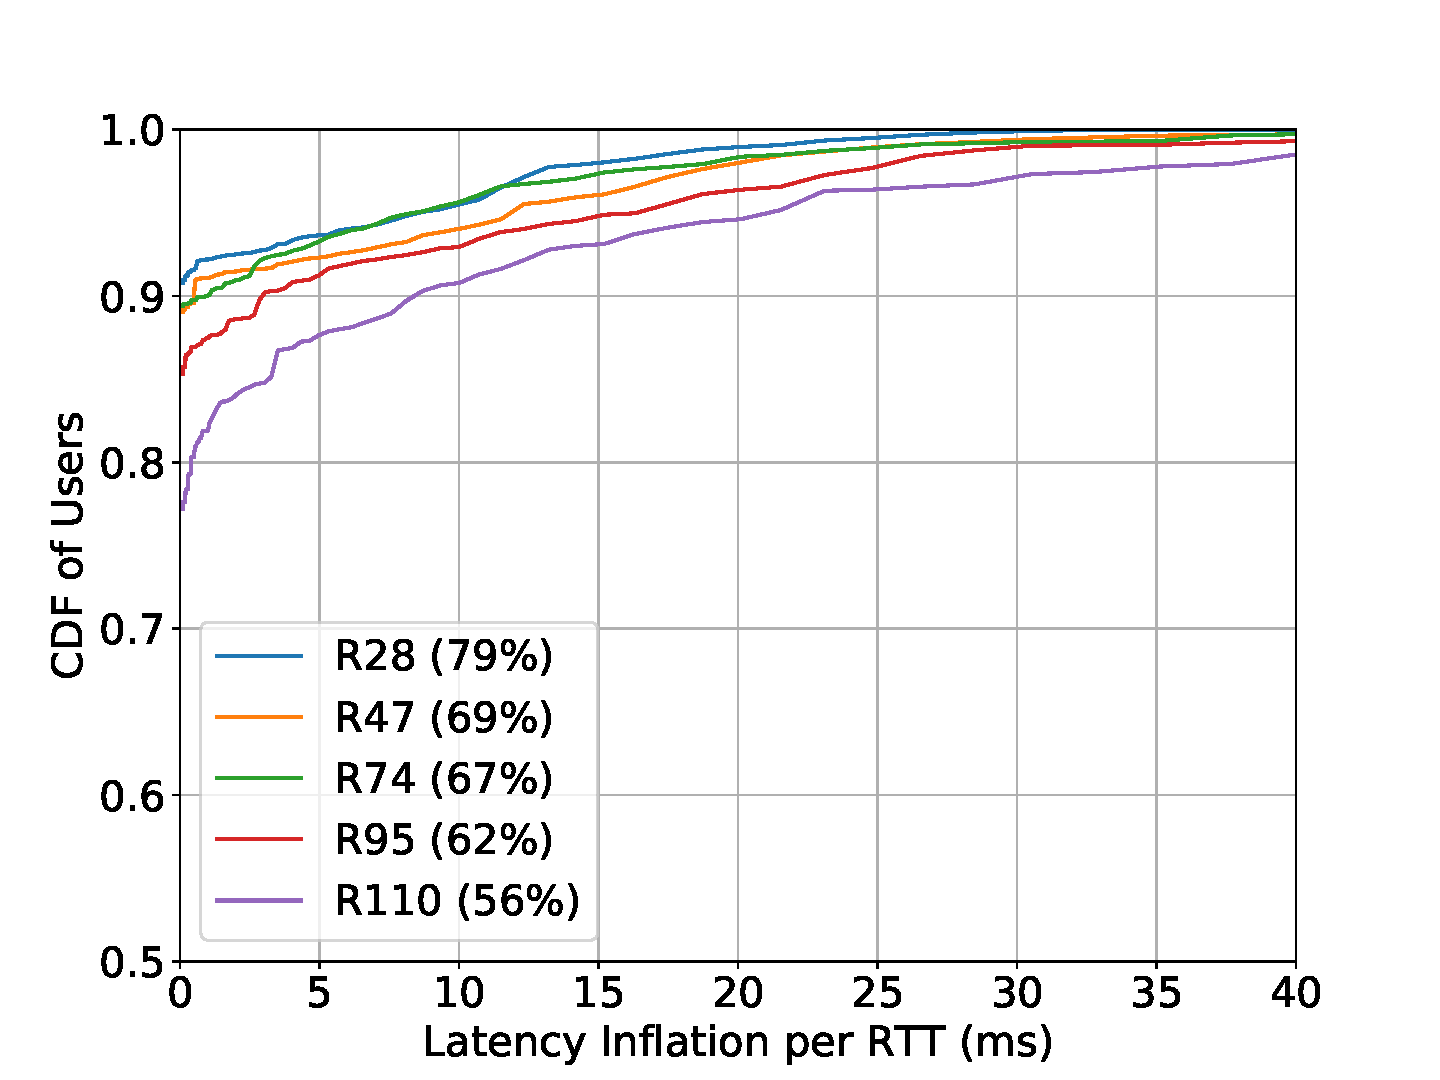
\includegraphics[width=\linewidth]{figures/inflation_microsoft_root-a.pdf}
        \label{fig:inflation_microsoft_root-a}
    } \\
    \subfloat[]{
        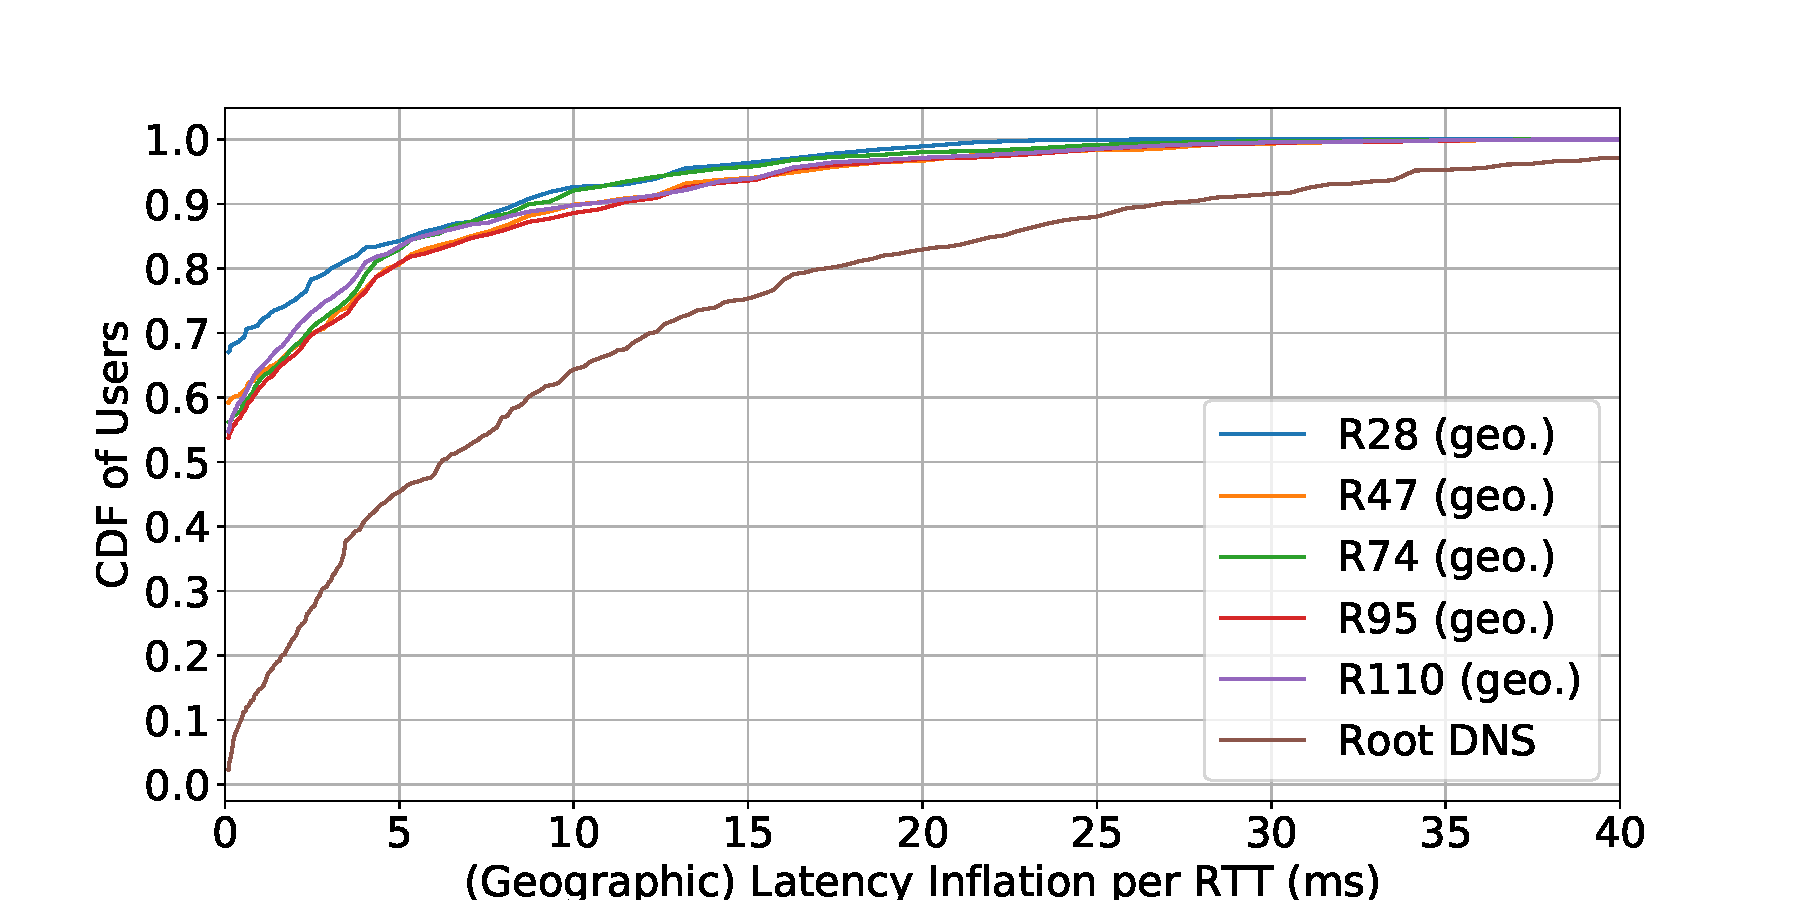
\includegraphics[width=\linewidth]{figures/inflation_microsoft_root-b.pdf}
        \label{fig:inflation_microsoft_root-b}
    }
    \caption{Anycast path inflation measured using CDN server side logs (\ref{fig:inflation_microsoft_root-a}) and using geographic information (\ref{fig:inflation_microsoft_root-b}). Path inflation becomes more prevalent for larger deployments, but it is still quite small for most users. Path inflation in the anycast CDN is also much less common than in the root DNS.}
    \label{fig:inflation_microsoft_root}
\end{figure}

\subsection{Comparison}\label{comparison-3}

Having presented the analysis of anycast for two different services, we
now take a step back and summarize the key differences in efficiency.
One problem anycast introduces, path inflation, is much lower for the
anycast CDN than in the roots. Not only do users tend to go to closer
CDN sites than they do root DNS sites, but these paths are also rarely
inflated at all. This result is not surprising, when we consider how
much more latency matters in a web page load, than does root DNS
inflation. Although root DNS queries see greater inflation (and see
inflation more often), when inflation does occur for CDN queries, it
hurts user-experienced latency (here, page load-time) much more than
equivalent inflation for DNS root queries. Combined, these observations
suggest the CDN is working harder to control cases of sub-optimal
routing, since users feel the pain.

Another way of measuring inefficiency in routing is to look at where
queries are being routed with respect to users generating those queries,
without paying mind to incurred latency. Observing that most users reach
their closest or second closest site suggests an anycast deployment is
`efficient'. We explore this notion further in \Cref{ap:distance_ranks}.
However, geography is not a perfect indicator of efficiency. An
assessment of anycast routing inefficiency based solely on geography
neglects geopolitical restrictions, physical restrictions
(e.g.~topography), and routing constraints.

\section{Discussion}\label{discussion}

\label{sec:discussion}

Anycast performance is interesting to assess in its own right, even
without attention to how that performance affects end users. However,
the magnitude of \emph{problems} caused by anycast's inefficiencies are
proportional to their effect on end users. Hence, conclusions we draw
about ``what should be done'' in the face of such inefficiencies depend
on the service the anycast is providing. This principle extends beyond
anycast and should be applied to any system.

Recent work has suggested that anycast inefficiency (path inflation) is
a serious problem, based on analysis of root DNS deployments
\cite{li_levin_spring_bhattacharjee_2018}. The authors argue that adding
more sites may hurt rather than help deployments (due to inflation), and
suggest that solutions either involve cooperation from a large ISP or
widespread modifications to BGP policy. The root DNS is a vital,
heterogeneous anycast deployment, and data is easy to access. However,
conclusions based on this data may not apply in other contexts beyond
the root DNS.

We build on this work by investigating both root DNS and an additional
type of anycast deployment -- CDNs. Considering the behavior of each
deployment in the context of its role reveals a richer picture of
anycast behavior than can be learned from studying root DNS alone,
especially since inflation and efficiency depend mostly on deployment
details.

Each letter root and the CDN are run by different organizations and so
have different operational budgets, deployment strategies, and
peering/routing strategies. These differences mean that comparisons
between, for example, D root and F root may be uncontrolled, in the
sense that they vary in multiple dimensions outside the one of interest.
For example, \Cref{fig:api_per_rtt_roots} might suggest that more sites
leads to more inflation. However, asserting this ignores the fundamental
differences among the root letter deployments.

Our analysis of CDN data provides evidence that network operators can
control anycasts' inefficiencies, even though these inefficiencies are
quite prevalent in the root DNS. Moreover, inefficiency does not tell a
complete story, since systems such as the root DNS do not have a strong
incentive to decrease latency. DNS caching means that users experience
nearly no latency from root DNS queries, and even eliminating path
inflation in the root is unlikely to be noticed. Conversely, the low
latency and inflation achieved by the CDN results from extensive
resources for infrastructure and peering, and the constant engineering,
monitoring, and automation for network optimization and debugging. We
hope others will take our results into consideration in future studies
discussing anycast performance for services, including the root DNS.

\section{Related Work}\label{related-work-1}

\label{sec:related}

IP anycast performance is usually studied in the context of two
applications: the root DNS servers, and CDNs. In addition to these
topics, we discuss studies of popular recursives, and user-centric
measurements of web performance.

\subsection{Root DNS Anycast}\label{root-dns-anycast-2}

\label{sec:related_root_dns_anycast}

The performance of anycast in the context of root DNS is generally
gauged by anycast's ability to balance load among server sites or
provide low latency to users. Previous work looked at DDoS attacks on
the root name server infrastructure, and showed that anycast is a
helpful defense mechanism against such attacks
\cite{sarat2006use, moura2016anycast}.

Other work looked at anycast performance and found it is decent for most
roots \cite{sarat2006use} but is related to good geographic locations of
anycast sites and peering strategies \cite{de2017anycast}. These
findings coincide with an earlier study that concluded the performance
of anycast is intrinsically linked to deployment strategy
\cite{ballani2006measurement}. Towards assessing how size of the
deployment correlates to performance, previous work suggested that as
few as 12 sites can provide ``good'' latency to users
\cite{de2017anycast}.

A final line of work looked at the \emph{efficiency} of anycast latency,
suggesting that more sites decrease efficiency
\cite{li_levin_spring_bhattacharjee_2018}. Many studies quantified
latencies to various root servers, and noted how these compare to the
(optimal) latency of the closest unicast alternative for the user who
issued the query
\cite{colitti2006evaluating, de2017anycast, liang2013measuring}.

Our paper focuses on performance, considering latency and efficiency,
and does not consider DDoS mitigation. We are the first to examine two
different applications to see how the importance of latency drives CDNs
to greater efficiency. Finally, we show that efficiency is less
important than absolute latency, suggesting that emphasis on
inefficiency in larger deployments is perhaps misplaced.

\subsection{CDN Anycast}\label{cdn-anycast-2}

\label{sec:related_cdn_anycast}

Some CDNs \cite{calder2015analyzing,edgecast_anycast,amazon_cloudfront}
use IP anycast to augment their serving infrastructure. The simplicity
of IP anycast for CDNs comes at the cost of having coarse grained
control over where user queries land; for example, shifting user load
between nodes during peak hours is a challenging problem. Some CDNs use
DNS redirects at ADNS servers to shift load among anycast nodes
\textbackslash{}cite\{alzoubi2011practical, \{flavel2015fastroute\}.
Previous work analyzed what latency CDN users are achieving, compared to
optimal, when being routed to anycast nodes and found that 10\% of users
experience a latency inflation of at least 100 ms
\cite{calder2015analyzing}. Our work builds on this result by instead
focusing on how the size of the deployment affects user experience.

\subsection{Recursive Resolvers and the Benefits of Caching and
Latency}\label{recursive-resolvers-and-the-benefits-of-caching-and-latency}

\label{sec:related_recursive_resolver_caches}

Similar to the recursive analysis conducted here, others have looked at
DNS traffic on a small network and found that 16\% of queries resulted
in queries to the root, most of which were for invalid domains
\cite{jung2002dns}. As this study is quite old, it is no surprise that
this rate has decreased (recall we observed 1.5\% of queries resulted in
queries to the root) since browser designers and network engineers
understand the importance of caching. Previous work also looked at
traffic between a neighborhood and a recursive and analyzed statistics
of DNS exchanges occurring over it including DNS transaction latencies
\cite{callahan2013modern}. Some previous work looked at certain
pathological behaviors of popular recursives, and the implications these
behaviors have on root DNS load times
\cite{yu2012authority, lentz2013d}.

Work has examined recursive selection across multiple authoratives,
showing the extent to which preferences for lower latency shift traffic
\cite{Mueller17b}. Our work looks at how authoritative anycast systems
may optimize latency.

\subsection{Web Performance}\label{web-performance}

\label{sec:related_web_performance}

Many studies characterize web performance and consider DNS, although
none consider root DNS specifically. Researchers have characterized web
performance bottlenecks in (at the time) new broadband networks, and
found that latency was the main bottleneck for page load time when the
user's bandwidth exceeds 16 Mb/s \cite{sundaresan2013web}. However, the
study did not realistically simulate a page load and did not analyze the
effect of having multiple DNS resolutions per page. Others analyzed how
each step of a page load contributes to the aggregate PLT using a tool
designed in-house \cite{asrese2016wepr}. This work, however, did not
conduct a large measurement campaign and did not include information
about multiple DNS lookups per page. Finally, HTTP Archive
\cite{http_archive} is an ongoing effort to characterize web
performance, but only measures from a single vantage point.

\iffalse
(studies looking at anycast in context of root DNS servers) Anycast
Performance, Problems and Potential how many sites are enough? A
measurement based deployment proposal for IP Anycast Evaluating the
Effects of Anycast on DNS Root Nameservers Measuring Query Latency of
Top Level DNS Servers Anycast vs.~DDoS: Evaluating the November 2015
Root DNS Event On the Use of Anycast in DNS (studies looking at anycast
in context of CDNs) fastroute A Practical Architecture for an Anycast
CDN Edgecast paper that hasn't been released yet Analyzing the
Performance of an Anycast CDN (studies looking at recursive
resolvers/caching) (maybe) John's TR of how different resolvers query at
different times On Modern DNS Behavior and Properties DNS Performance
and the Effectiveness of Caching D-mystifying the D-root Address Change
Authority Server Selection of DNS Caching Resolvers Recursives in the
Wild: Engineering Authoritative DNS Servers (studies looking at web
performance/how user caching effects it) Measuring and mitigating web
performance bottlenecks in broadband access networks WePR: A tool for
Automated Web Performance Measurement Demystifying Page Load Performance
with WProf Practical Challenge Response for DNS DNS Resolvers Considered
Harmful Studies looking at root servers and queries that land at them On
eliminating root nameservers from the DNS DNS Measurements at a Root
Server A Day at the Root of the Internet Internet Usage Users spend
average 6+ hrs / day on the Internet (hootsuite) Statistics drawn from
various organizations Users spend average 30+ minutes on various forms
of social media per day (although knowing sources is behind a paywall?)
Americans spend average 3+ hrs/day on the Internet (digital center)
Survey data from 2000 U.S. households Usage statistics for various
social media/entertainment things, e.g. \textasciitilde{}30 minutes/day
for youtube Similarweb Pays for data from the source maybe? Also has a
web extension that users can download, which records statistics

\fi

\section{Conclusion}\label{conclusion-1}

Anycast is widely used in many systems to provide content to users, but
it has come under fire for routing users to suboptimal sites. Research
usually uses the root DNS to demonstrate this suboptimality, but users
rarely interact with the root DNS since caching is so effective. Taking
a user-centric approach to studying anycast performance, we show that
root DNS performance doesn't matter for users and that for anycast CDNs,
performance can be quite good. Although inefficiencies do exist, anycast
still does a good job routing users to sites.

{\small\balance\bibliography{mybib.bib}}
\appendix
\newpage

\section{Quantifying the Impact of Methodology
Decisions}\label{quantifying-the-impact-of-methodology-decisions}

When analyzing latency and inflation, we often make assumptions or
choose to conduct analysis a certain way. In what follows, we justify
our various assumptions and pre-processing steps, analyze the effects of
these assumptions on our results, and, when possible, offer alternative
methods of performing the analysis.

\subsection{Effect of Removing Invalid TLD
Queries}\label{effect-of-removing-invalid-tld-queries-1}

\label{ap:invalid_queries}

In \Cref{sec:root_dns_latency} we estimate the amount of latency users
experience due to the root DNS by amortizing queries over user
populations. Out of 51.9 billion daily requests to all roots, we observe
31 billion daily requests for bogus domain names and 2 billion daily
requests for PTR records. We choose to not count these towards user
latencies (\ie towards a recursive's daily query count), because we
believe many of these queries do not lie on the critical path of user
applications, and so do not cause user-facing latency. This decision has
a significant effect on conclusions we can draw, increasing daily median
latencies due to root DNS resolution by \(30\times\).

We base this decision on prior work on the nature of queries with
invalid TLDs landing at the roots. ICANN has found that 28\% of queries
for non-existent domains at L-root result from captive-portal detection
algorithms in Chromium-based browsers \cite{akplogan2020covid}.
Researchers at USC have found that more than 90\% of single-label
queries at the root match the Chromium captive-portal pattern
\cite{broot_invalid_queries}. We remove captive-portal detection queries
from user latency because it occurs on browser startup and network
reconnect, not during regular browsing, and it can occur in parallel
with browsing.

Some might argue that queries for invalid TLDs \emph{are} associated
with user latency because typos for URLs (when typing into a browser
search bar, for example) cause users to experience latency and generate
a query to the root servers. However, typos only generate a query to the
root server if the TLD is misspelled (as opposed to the hostname). Hence
typos, in general, cause users latency, but only specific typos will
cause users \emph{root} latency. Moreover, others have found that
approximately 60\% of queries for invalid TLDs reaching root servers are
for domains such as local, no\_dot, belkin, and corp
\cite{gao2014reexamining}. It is unlikely these queries are caused by
typos, since they are actual (as opposed to misspelled) words and
resemble domains often seen in software or in corporate networks.
Chromium queries and queries for a certain set of invalid TLDs therefore
account for around 86\% of all queries for invalid TLDs at the roots,
suggesting the vast majority of queries we exclude are not directly
associated with user latency.

\begin{figure}
    \centering
    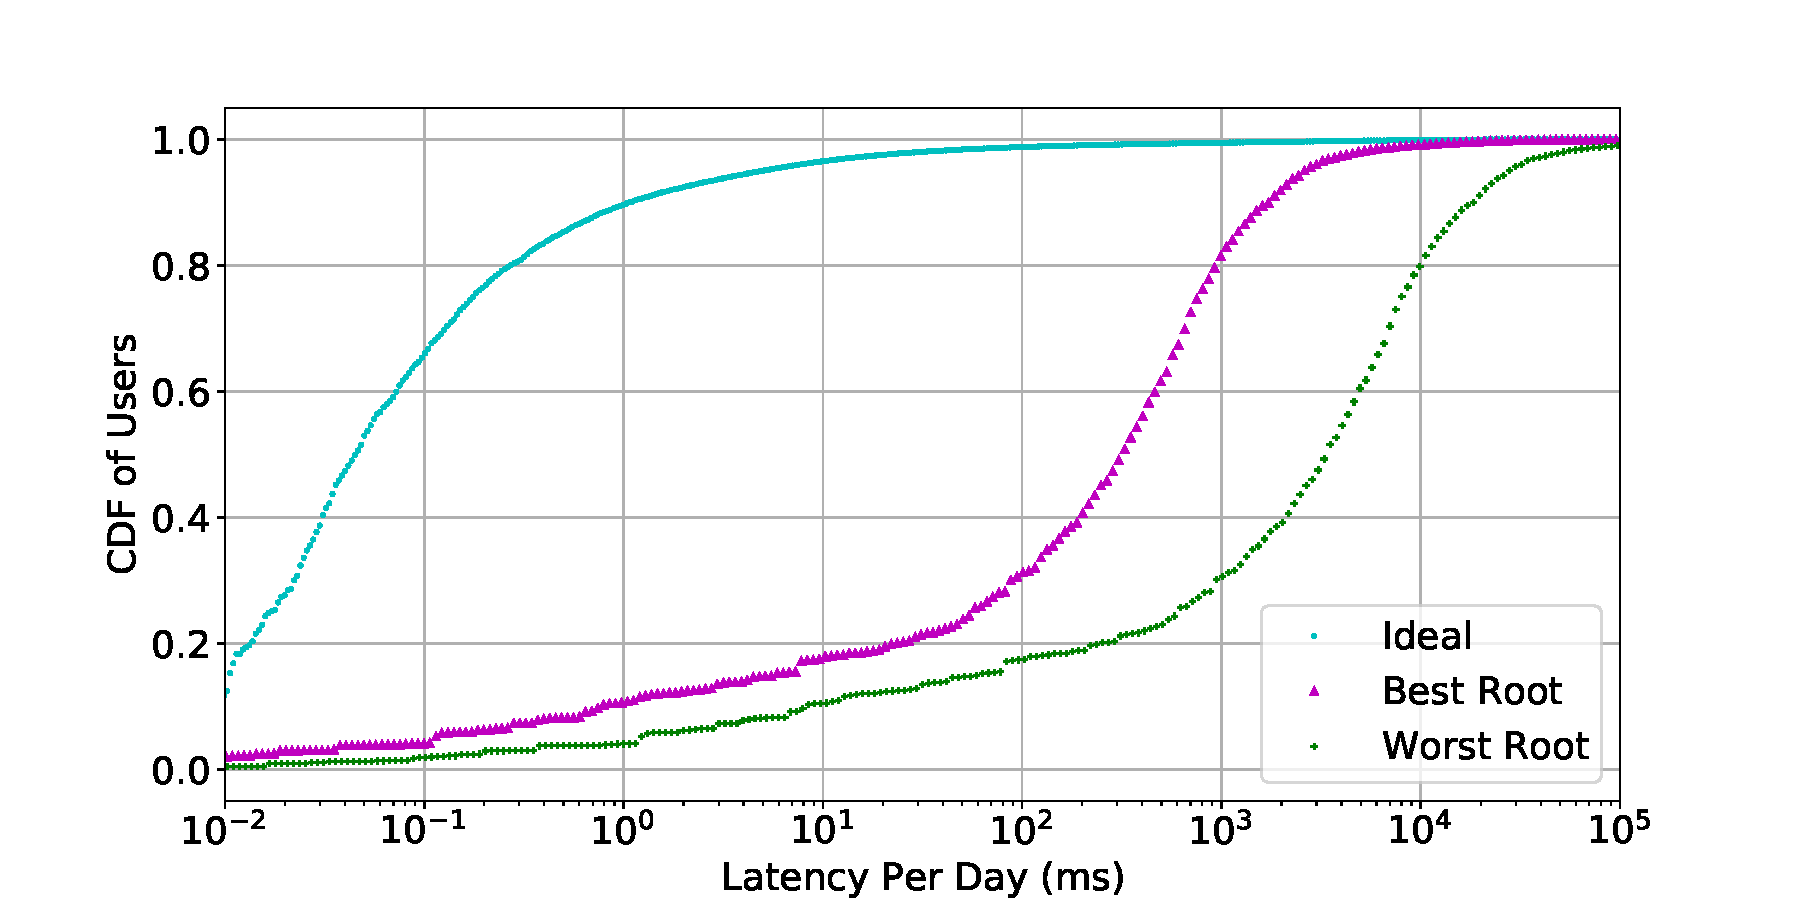
\includegraphics[width=\linewidth]{figures/include_invalid_daily_root_latency.pdf}
    \caption{Daily latency experienced by users due to the root DNS, calculated by amortizing root DNS requests over user populations, when including or excluding queries for invalid TLDs. Counting invalid queries drastically increases daily user latency estimates to 327 ms for Best Root (a 30-fold increase). }
    \label{fig:include_invalid_daily_root_latency}
\end{figure}

Nevertheless, it is still valuable to assess how including these queries
for invalid TLDs changes the conclusions we can make about root DNS
latency experienced by users.
\Cref{fig:include_invalid_daily_root_latency} shows daily user latencies
due to root DNS resolution when we include requests for invalid TLDs and
PTR records in daily query volumes. Using the `Best Root' latency, users
experience 327 ms of root latency at the median -- about 30\(\times\)
more than when we exclude requests for invalid queries
(\cref{sec:root_dns_latency}). This drastic 30-fold difference is
surprising given we only (roughly) double the amount of queries by
including invalid queries. The difference is best explained by the fact
that a majority of invalid queries are generated by /24s with a large
number of users. Since the y-axis of
\Cref{fig:include_invalid_daily_root_latency} is the number of users
(not /24s), counting invalid queries shifts the graph far to the right.
Hence, counting invalid queries drastically affects the conclusions we
can draw. For example, there is a 3 \emph{second} difference at the
median between Best Root and Worst Root. This 3 second difference is
harder to dismiss than the corresponding 78 ms difference between Best
Root and Worst Root medians in \Cref{fig:user_root_latency_per_day}.
However, this three seconds \emph{per day} is still quite small (less
time than a single page load \cite{http_archive}), so the major
conclusions reached in \Cref{sec:root_dns_latency} still apply.

\subsection{Representativeness of Daily Root Latency
Analysis}\label{representativeness-of-daily-root-latency-analysis}

\label{ap:join_by_24} In \Cref{sec:root_dns_latency} we estimate the
amount of latency users experience due to the root DNS by amortizing
queries over user populations. To obtain estimates of user populations,
we obtain counts of users of a large CDN who use recursives
(\cref{sec:root_dns_data_sources}). Naturally recursives used by users
of the large CDN and recursives seen in DITL do not overlap perfectly.
To increase the representativeness of our analysis, we aggregate CDN
user counts and DITL query volumes by resolver /24, and join the two
data sets on /24 to create the DITL\(\cap\)CDN data set. The intuition
behind this preprocessing step is that IP addresses in the same /24 are
likely colocated, owned by the same organization, and act as recursives
for similar sets of users. We now justify this decision and discuss the
implications of this preprocessing step on the results presented in
\Cref{sec:root_dns_latency}.

In \Cref{tab:dataset_matching_statistics_by_32} we summarize the extent
to which the recursives seen by the CDN are representative of the
recursives seen in DITL, and vice-versa, without aggregating by /24. We
also display corresponding statistics (from
\cref{tab:dataset_matching_statistics}) when aggregating by /24 for
comparison in parentheses. Clearly joining by /24 makes a significant
difference, increasing various measures of overlap uniformly by tens of
percents and in certain cases by up to 64\%.

\begin{table}[]
\centering
\resizebox{\linewidth}{!}{%
\begin{tabular}{|l|l|l|}
\hline
\textbf{Data Set}                            & \textbf{Statistic} & \textbf{Percent Overlap} \\ \hline
\multirow{4}{*}{DITL $\cap$ CDN}             & DITL Recursives          & 2.45\% (29.3\%) of DITL Recursives                            \\ \cline{2-3} 
                                             & DITL Volume        & 8.4\% (72.2\%) of DITL Query Volume                            \\ \cline{2-3} 
                                             & CDN Recursives           & 41.9\% (78.8\%) of CDN Recursives                           \\ \cline{2-3} 
                                             & CDN Volume         & 47.05\% (88.1\%) of CDN Query Volume                            \\ \hline
\multirow{4}{*}{DITL $\cap$ CDN $\cap$ RIPE} & DITL Recursives          & .07\% (.14\%) of DITL Recursives                              \\ \cline{2-3} 
                                             & DITL Volume        & 11.8\% (20.7\%) of DITL Query Volume                           \\ \cline{2-3} 
                                             & CDN Recursives           & .01\% (.34\%) of CDN Recursives                              \\ \cline{2-3} 
                                             & CDN Volume         & .62\% (54.6\%) of CDN Query Volume                            \\ \hline
\end{tabular}%
}
\caption{Statistics displaying the extent to which the recursives of users in a large CDN overlap recursives seen in the 2018 DITL captures without users and volumes by /24. Also shown in parentheses are corresponding statistics when joining by /24. Joining the data sets by /24 increases most measures of representation by tens of percents, with some measures increased by up to 64\%.}
\label{tab:dataset_matching_statistics_by_32}
\end{table}

As an analogy to \Cref{fig:user_root_latency_per_day}, in
\Cref{fig:user_root_latency_per_day_by_32} we show daily latency
experienced by users of a large CDN due to root DNS latency
\emph{without} aggregating query and user statistics by /24. The median
daily latency when users use `Best Root' is only .46 ms -- roughly one
\(30^{th}\) of the estimate obtained when aggregating statistics by /24.
This small daily user latency makes sense, given that we only capture
8.4\% of DITL volume without joining the datasets by /24
(\cref{tab:dataset_matching_statistics_by_32}).

\begin{figure}
    \centering
    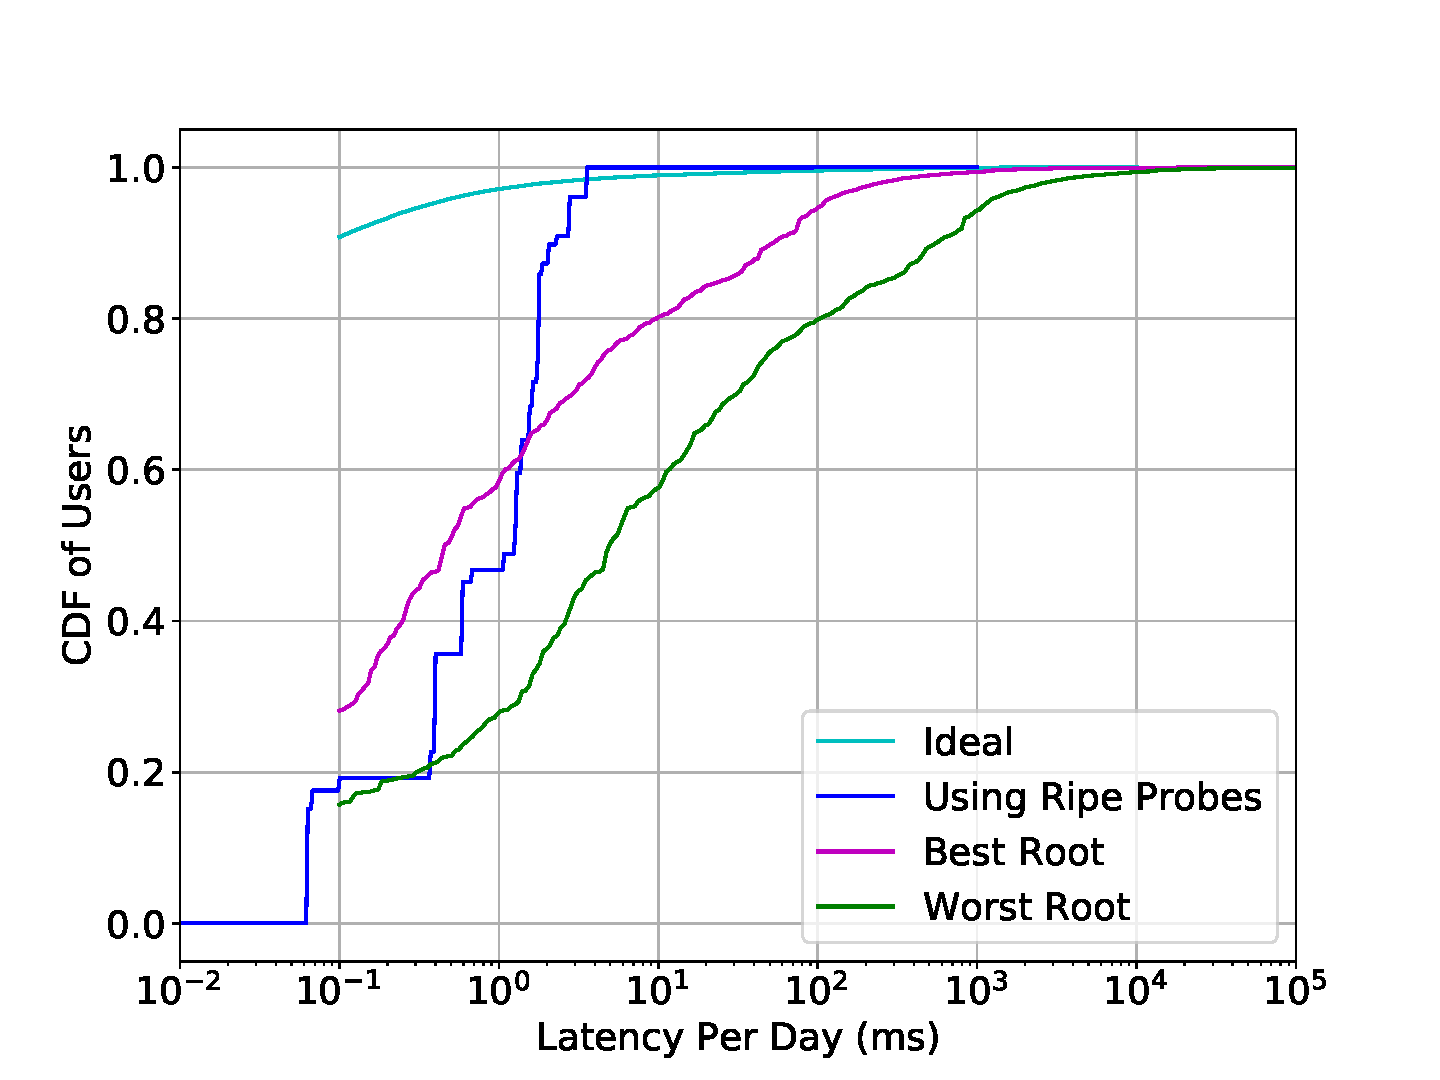
\includegraphics[width=\linewidth]{figures/user_root_latency_per_day_by_32.pdf}
    \caption{A CDF of approximate latency a user experiences due to root DNS resolution, per day, without joining recursives in DITL with recursives seen by the CDN by /24. This unrepresentative analysis yields an estimate of daily user latency far lower than in \Cref{sec:root_dns_latency}. }
    \label{fig:user_root_latency_per_day_by_32}
\end{figure}

\Cref{tab:dataset_matching_statistics_by_32} and
\Cref{fig:user_root_latency_per_day_by_32}, demonstrate that the
decision to aggregate statistics and join DITL captures with CDN user
counts by /24 led to both much greater representativeness of the
analysis and very different conclusions about daily latency experienced
by users due to the root DNS. We would now like to justify this decision
using measurements. If, as we assume, IP addresses in the same /24 are
colocated, they are probably routed similarly. Prior work has shown that
only a small fraction of anycast paths are unstable \cite{wei2017does},
and so we expect that, over the course of DITL, IP addresses in the same
/24 reach the same anycast sites.

As a way of quantifying routing similarity in a /24, in
\Cref{fig:routing_similarity_by_24} we show the percent of queries from
each /24 in DITL that do not reach the most ``popular'' anycast site for
each /24 in each root deployment. Specifically, for each root letter and
for each /24 that queried that root letter in DITL, we look at how
queries from the /24 are distributed among sites.

Let \(\mathnormal{q^{k}_{ij}}\) be the number of daily queries from IP
\(\mathnormal{i}\) in /24 \(\mathnormal{k}\) toward anycast site
\(\mathnormal{j}\). We then calculate the fraction of queries that do
not visit the most ``popular'' site as

\begin{equation}
f^k = 1 - \underset{i}{\sum} \frac{q^k_{i j_{F}}}{Q^k} 
\end{equation}

where \(\mathnormal{j_F}\) is the favorite site for /24
\(\mathnormal{k}\) (\ie the site the /24 queries the most), and \(Q^k\)
is the total number of queries from /24 \(\mathnormal{k}\). We plot
these fractions for all /24s in DITL, and for each root
deployment.\footnote{We do not include /24s that had only one IP from
  the /24 visit the root letter in question.}

For more than 80\% of /24s, all queries visit only one site per root
letter, suggesting that queries from the same /24 are routed similarly.
This analysis is slightly biased by the size of the root deployment. For
example, two IP addresses selected at random querying B-root would hit
the same site half the time, on average. However, even for L root, with
138 sites, more than 90\% of /24s direct all queries to the most popular
site. We believe \Cref{fig:routing_similarity_by_24} provides evidence
that recursives are located near each other, and hence serve similar
sets of users.

Even queries from a single IP within a /24 may reach multiple sites for
a single root over the course of the DITL captures. Such instability can
make routing look less coherent across IP addresses in a /24, even if
they are all routed the same way. Controlling for cases of changing
paths for the same IP makes intra-/24 routing even more coherent. If we
let the distribution of queries generated by an IP address to a root be
a point mass, with all the queries concentrated at that IP addresse's
favorite site, all queries from more than 90\% of all /24s in all roots
are routed to the same site (not shown).

\Cref{ap:apnic_root_latency_per_day} offers further evidence this
decision is justified, since it corroborates our results regarding daily
user root latency using very different methodology. Specifically,
without relying on aggregating statistics by /24 or using CDN user
counts, we reach similar quantitative and qualitative conclusions about
daily user latency experienced due to the root DNS.

\begin{figure}
    \centering
    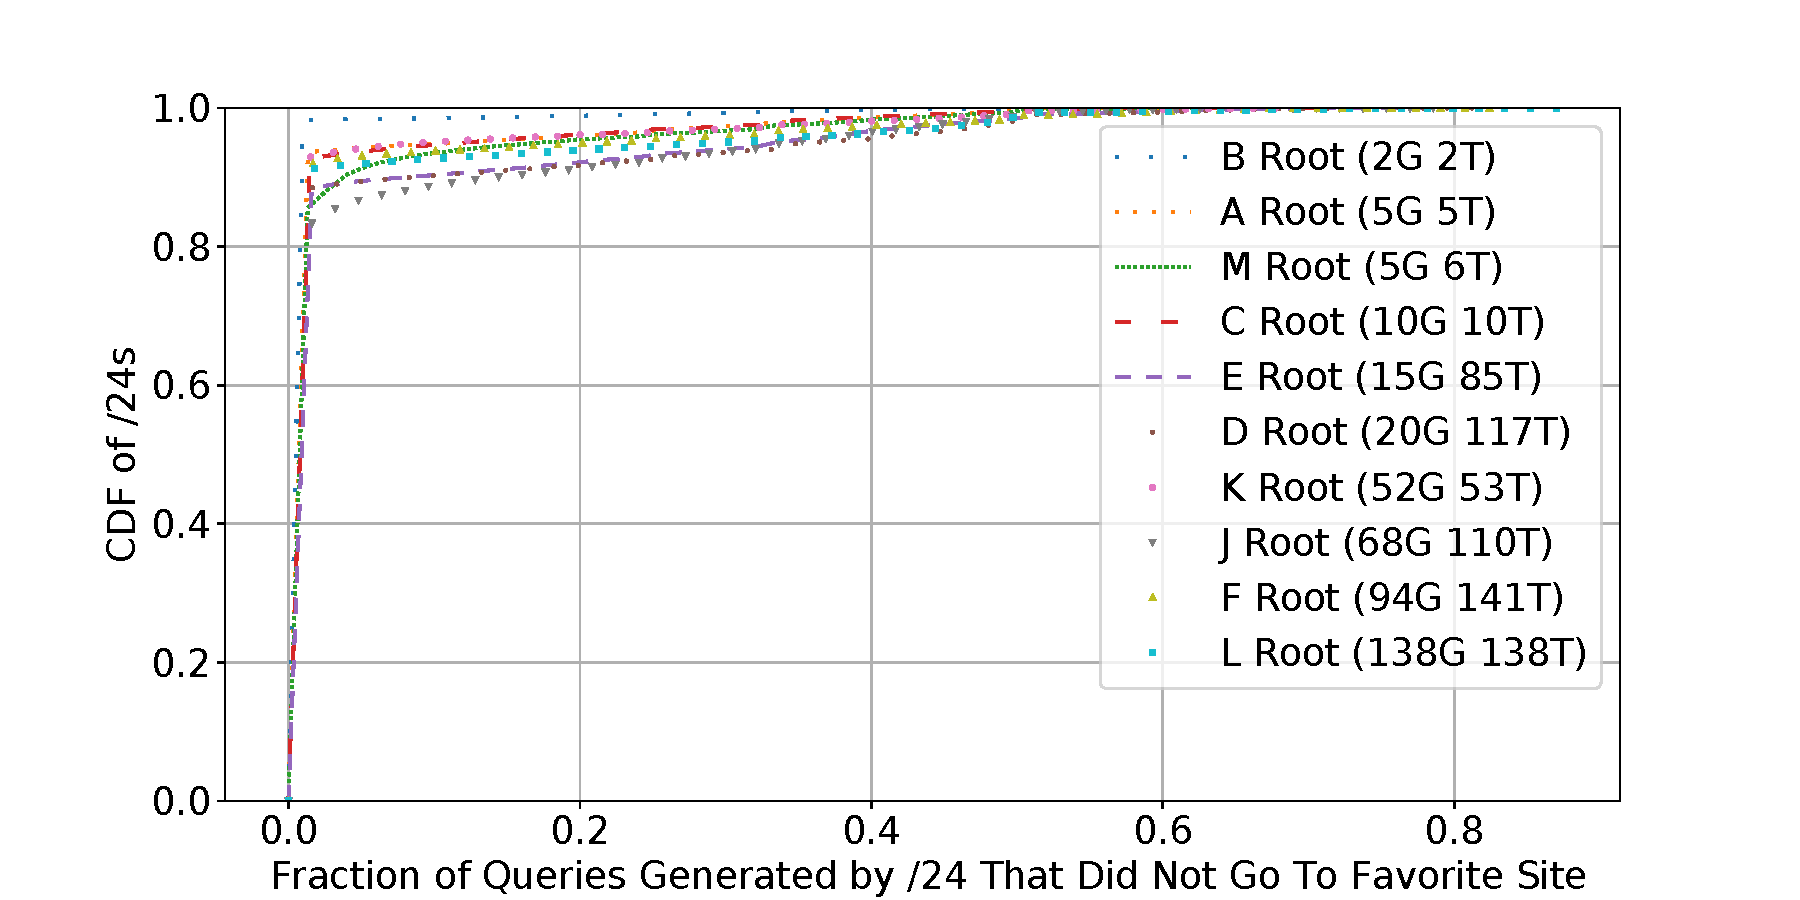
\includegraphics[width=\linewidth]{figures/routing_similarity_by_24.pdf}
    \caption{Fractions of queries generated by /24s that do not hit the most popular site for each /24 and for each root letter in question. For all root letters, more than 80\% of /24s have all queries visit the most popular site, suggesting queries from the same /24 are routed similarly.}
    \label{fig:routing_similarity_by_24}
\end{figure}

\subsection{Revisiting Root Latency Experienced per
Day}\label{revisiting-root-latency-experienced-per-day-1}

\label{ap:apnic_root_latency_per_day}

In \Cref{sec:root_dns_latency} we estimate the amount of latency users
experience due to the root DNS by amortizing queries over user
populations. Unfortunately, we could not obtain user population
estimates for every recursive resolver, so we focused on a subset of
resolver for which we did have population data.

To complement the analysis in \Cref{sec:root_dns_latency}, we use
Internet user population estimates by AS from APNIC instead of CDN user
counts to amortize root DNS latency \cite{apnic_pop_est}. These
estimates were obtained by first gathering lists of IP addresses from
Google's Ad delivery network, separated by country. This distribution of
IP addresses was converted to a distribution of ASNs, and normalized by
country Internet-user populations. The major assumptions made when
generating the APNIC user counts are that Google Ad placement is uniform
across ASes within a country, and that both an AS and its users are
fully contained in a single country.

We use this dataset to amortize root DNS queries seen from ASes over
user populations. First, we use the TeamCymru IP to ASN mapping to map
IP addresses seen in the DITL captures to their respective ASs
\cite{teamcymru}, and accumulate queries by ASN. We were able to map
99.4\% of IP addresses to an ASN seen in DITL, representing 98.6\% of
DITL query volume. Next, assuming recursives only serve users in the
same AS, we divide the number of daily queries seen in DITL from each AS
by the number of users in that AS to obtain the number of daily queries
per user. The assumption that recursives are in the same AS as the users
they serve is obviously incorrect for public DNS services, but we do not
make an effort to correct for these cases.

We plot the resulting latencies in \Cref{fig:apnic_daily_root_latency}
for Worst Root and Best Root, and include the corresponding lines using
CDN user estimates for reference (\cref{sec:root_dns_latency}).

\begin{figure}
    \centering
    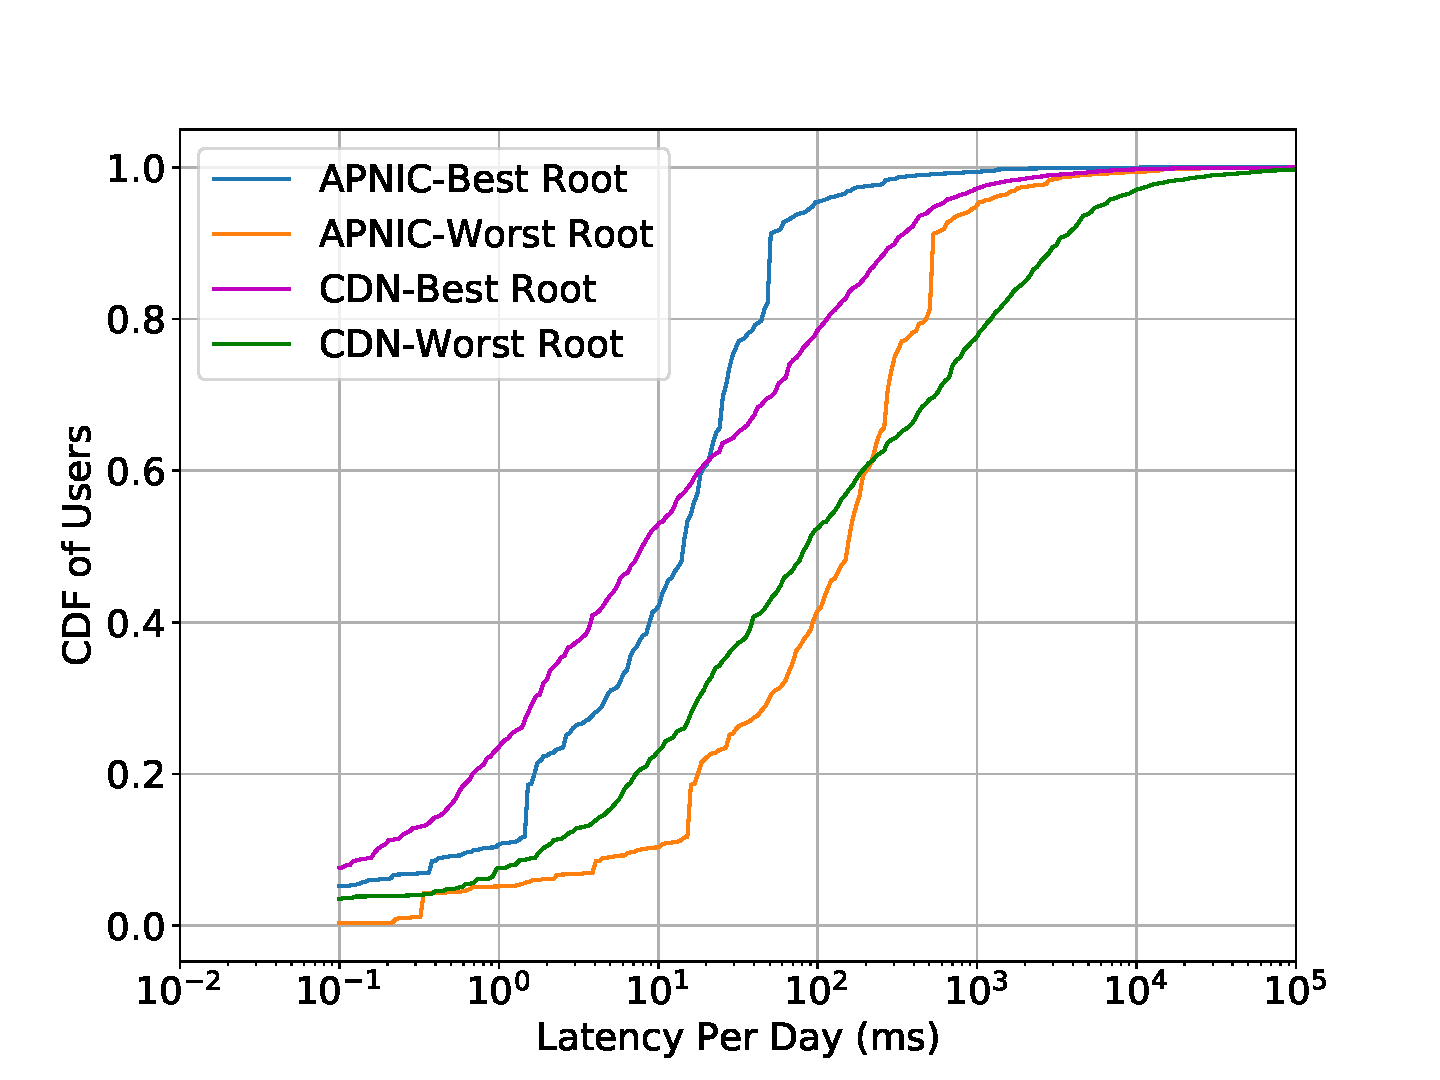
\includegraphics[width=\linewidth]{figures/apnic_daily_root_latency.pdf}
    \caption{Daily latency experienced by users due to the root DNS, calculated by amortizing root DNS requests over user populations. The APNIC and CDN lines use two different methods of estimating user counts behind each, but arrive at the same basic conclusion -- users do not experience much latency due to the root DNS.}
    \label{fig:apnic_daily_root_latency}
\end{figure}

Using APNIC's user estimates, users experience approximately the same
daily user latency at the median (about 15 ms for Best Root), and much
less daily user latency in the tail. This result is interesting since
the same conclusions can be drawn about daily root DNS latency
experienced by users, using two very different methods of amortizing
root latency over user populations. This method of computing root DNS
latency experienced by users reaffirms that users do not experience much
latency due to the root DNS.

\subsection{Estimating the Number of RTTs in a Page
Load}\label{estimating-the-number-of-rtts-in-a-page-load-1}

\label{ap:num_rtts_ppl}

To estimate the latency a user experiences due to anycast
(\cref{sec:anycast_cdn_latency}), we first must estimate the number of
RTTs required to load a typical web page hosted by the large CDN. We
provide an estimate of the number of RTTs based on modeling and
evaluation of a set of 1,000 web pages using Selenium (a headless web
browser).

CDN latency occurs when a user downloads web objects via HTTP. For a
single TCP connection, the number of RTTs during a page load depends on
the size of files being downloaded. This relationship is approximated by

\begin{equation}
\label{eq:rtt_calculation}
N = \lceil log_{2}{\frac{D} {W}} \rceil
\end{equation}

where \(\mathnormal{N}\) is the number of RTTs, \(\mathnormal{D}\) is
the total number of bytes sent by the TCP connection from the server to
the user, and \(\mathnormal{W}\) is the initial congestion window size
in bytes \cite{Heidemann97b,Cardwell00a}. Although \(\mathnormal{W}\) is
set by the server, a majority of web pages set this value to
approximately 15 kB \cite{iwIMC17}, so we use this value. (We do not
consider QUIC in detail here, but with its larger initial window it will
see fewer RTTs.)

In \Cref{sec:performance_comparison} we aim to show CDN latency per page
load is orders of magnitude more than root DNS latency per page load, so
we make the following assumptions to establish a \emph{lower bound} on
\(\mathnormal{N}\):

\begin{enumerate}


\item The connection is limited by $\mathnormal{W}$, as opposed to the user's receive window. Connections are often limited by processing resources and serial requests \tbd{cite}, rather than the congestion window.
\item TCP is always in slow start mode, which implies the window size doubles each RTT. 
\item All TCP and TLS handshakes after the first do not incur additional RTTs (\ie they are executed in parallel to other requests).


\end{enumerate}

\begin{figure}
    \centering
    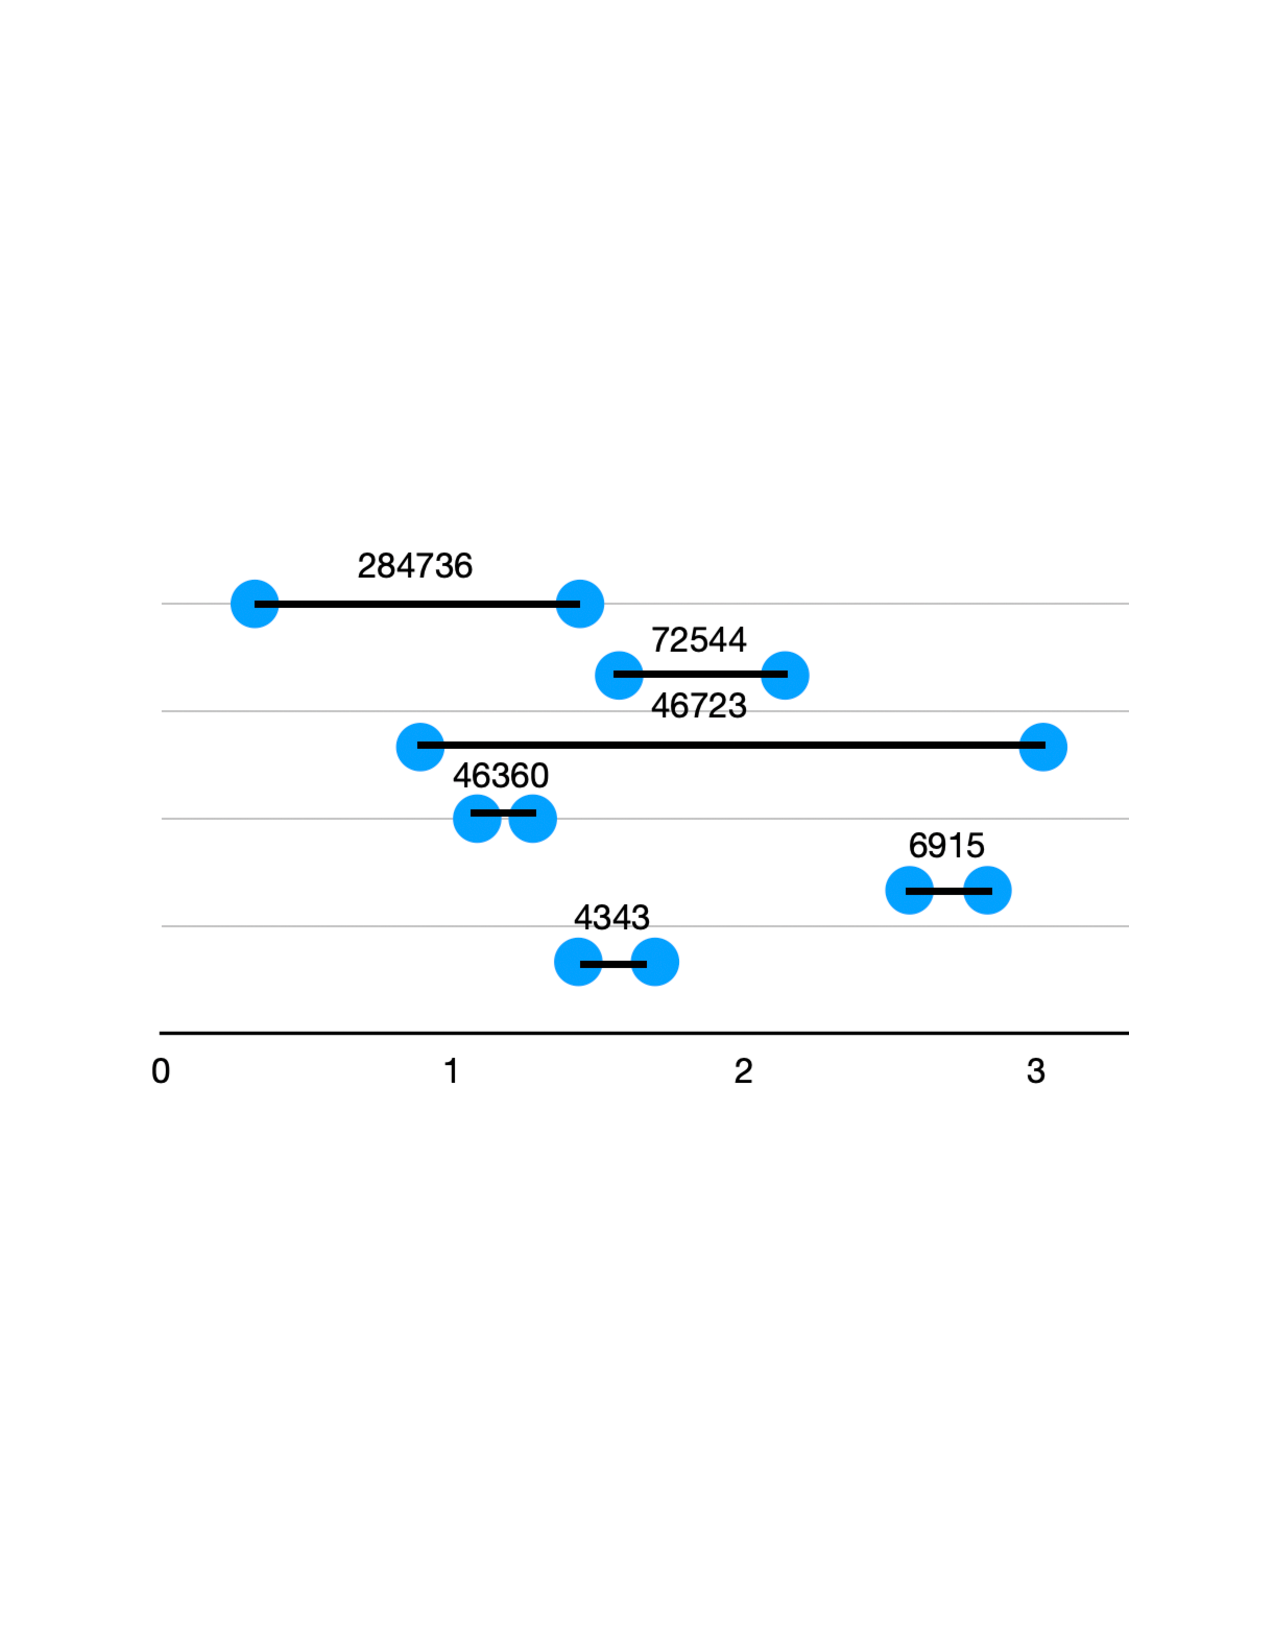
\includegraphics[width=\linewidth]{figures/multiple_tcp_connections.pdf}
    \caption{Example TCP connections for a web page loading. Each line is a TCP connection. Disregarding smaller downloads that overlap longer ones, we choose to accumulate RTTs associated with the 284 kB, 72 kB and 7 kB downloads.}
    \label{fig:multiple_tcp_connections}
\end{figure}

\iffalse

\textbackslash{}begin\{algorithm\}
\caption{Algorithm for pruning connections over which to accumulate RTTs. Larger connections are considered first, and RTTs for smaller connections are only accumulated if they do not overlap in time with any connection already being considered.}
\label{alg:rtt_pruning_algorithm}
\textbackslash{}begin\{algorithmic\}\footnote{We take care to ensure
  that user counts are not ``double counted'' across different resolver
  IP addresses in the same /24.} \State \(pruned\_connections\)
\(\gets\) \([max\_size(connections)]\) \State \(found\_new \gets False\)
\While{$found\_new$} \For{c $\in$ connections}
\If{not $overlap\_in\_time(pruned\_connections, c)$}
\State \(pruned\_connections\) \(\gets\) \(pruned\_connections\)
\(\cup\) c \State \(found\_new\) \(\gets\) True \State break \EndIf
\EndFor
\EndWhile
\textbackslash{}end\{algorithmic\} \textbackslash{}end\{algorithm\}

\fi

Modern browsers often open many TCP connections in parallel, to speed up
page loads. Summing up RTTs across parallel connections could therefore
drastically overestimate the number of RTTs experienced by the user.
\iffalse The algorithm we use to determine the connections over which we
accumulate RTTs is summarized in \Cref{alg:rtt_pruning_algorithm}.
\fi To determine which connections over which to accumulate RTTs, we
first start by only considering the connection with the most data. We
then iteratively add connections in size-order (largest to smallest)
that do not overlap temporally with other connections for which we have
accumulated RTTs. The `data size' of a connection may represent one or
more application-layer objects. This process of `pruning' connections is
illustrated in \Cref{fig:multiple_tcp_connections}. Disregarding the
smaller download sizes, we choose to accumulate RTTs associated with the
284 kB, 72 kB and 7 kB downloads.

We load two `classes' of web pages: the top-1000 web pages according to
GTMetrix \cite{gtmetrix} (once for each page) and nine web pages owned
by the large anycast CDN that we study in this paper (twenty times for
each page). We use Selenium and Chrome to open web pages and use Tshark
\cite{tshark} to capture TCP packets during the page load. For each web
page, we only capture packets until the loadEventEnd event has been
fired by the browser. When the load event ends, the whole page has
loaded, including all dependent resources such as stylesheets and images
\cite{web_api_load_event}. To calculate the total data size for each
connection, we use the ACK value in the last packet sent to the server
minus the SEQ value in the first packet received from the server. We set
\(\mathnormal{W}\) to 15 kB since a large fraction of web pages use this
value in practice \cite{iwIMC17}. We then calculate the number of RTTs
using \Cref{eq:rtt_calculation}, and add a final two RTTs for TCP and
TLS handshakes.

\begin{figure}
    \centering
    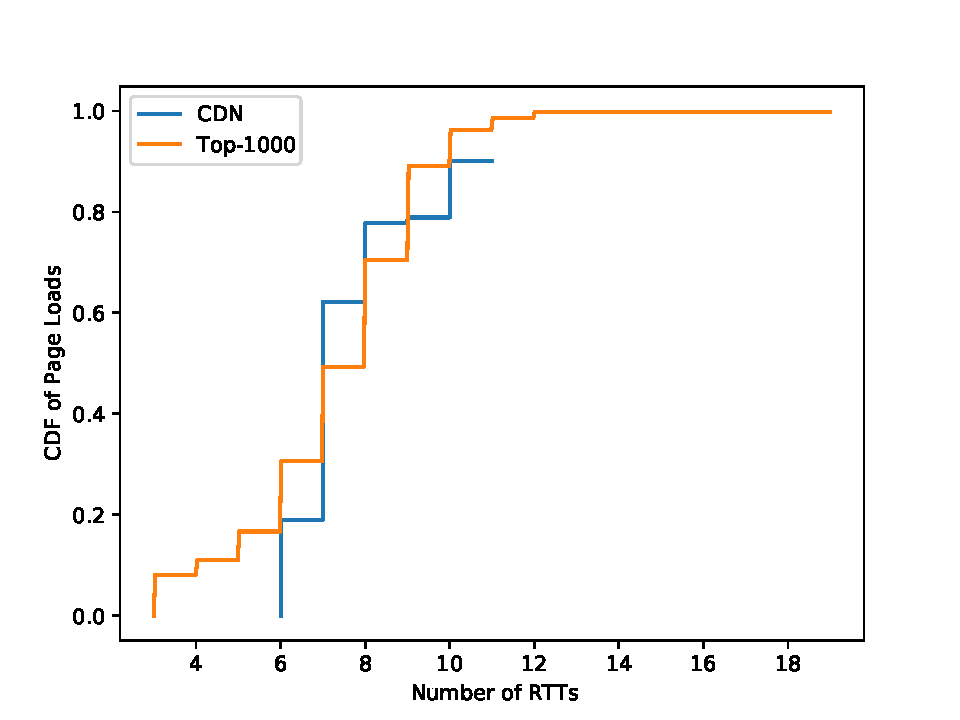
\includegraphics[width=\linewidth]{figures/rtts_per_page_load.pdf}
    \caption{The number of RTTs for page loads. CDN and Top-1000 refer to the types of pages being loaded. Only a few percent of CDN web pages are loaded within 10 RTTs and 90\% of all page loads are loaded within 20 RTTs.}
    \label{fig:rtts_per_page_load}
\end{figure}

The RTT estimates are shown in \Cref{fig:rtts_per_page_load}. As
\Cref{fig:rtts_per_page_load} demonstrates, only a few percent of CDN
web pages are loaded within 10 RTTs, and 90\% of all page loads are
loaded within 20 RTTs. Since we try to obtain a lower bound on the
number of RTTs per page load, we believe we are justified in using 10
RTTs in our analysis in \Cref{sec:anycast_cdn_latency}.

\subsection{CDN Path Inflation Over the Same Set of
Users}\label{cdn-path-inflation-over-the-same-set-of-users}

\label{ap:anycast_cdn_path_inflation_recalc}

\iffalse

Holding set of users constant across rings Case studies of why users
don't visit their closest site

\fi

In \Cref{fig:inflation_microsoft_root} we calculate path inflation for
users by subtracting latency to users' geographically closest
\feplural from user's achieved latency. However, some \metroas pairs do
not reach their closest \fe, so we can not calculate path inflation for
these users. This set of users for which we can calculate anycast path
inflation varies across rings.

We now calculate anycast path inflation for only those \metroas pairs
that have latency measurements to their closest \fe in all rings.
Limiting the analysis to a certain set of users allows a direct
comparison in inflation over the same set of users. The resulting path
inflations, and user representations (as a fraction of total users in
that ring) are shown in \Cref{fig:inflation_microsoft_same_users}. Path
inflation is slightly less prevalent for this set of users than all
users for which we can measure inflation
(\cref{fig:inflation_microsoft_root}). This result makes sense, since we
are excluding users that do not visit their closest \fe, and so are
inflated.

\begin{figure}
    \centering
    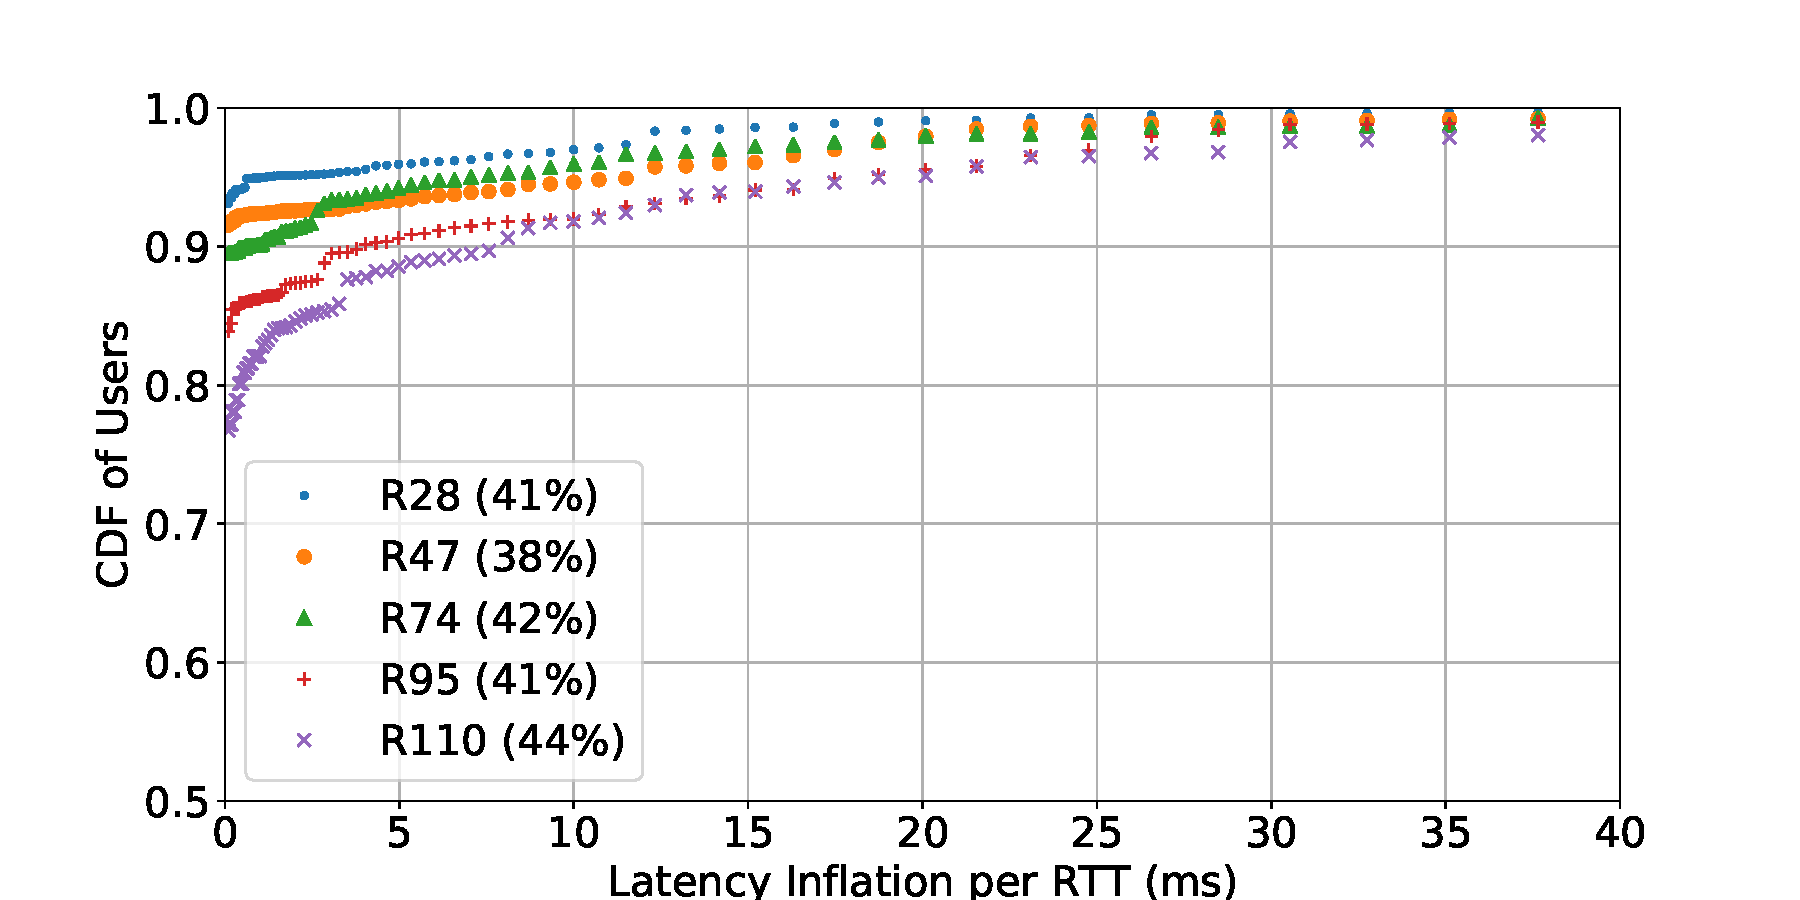
\includegraphics[width=\linewidth]{figures/inflation_microsoft_same_users.pdf}
    \caption{Anycast path inflation measured over rings for the same set of users. Path inflation is slightly less prevalent for this set of users than all users for which we can measure inflation (\cref{fig:inflation_microsoft_root}). This result makes sense, since we are excluding users that do not visit their closest \fe, and so are inflated.}
    \label{fig:inflation_microsoft_same_users}
\end{figure}

\section{Latency Measurements at a Recursive
Resolver}\label{latency-measurements-at-a-recursive-resolver-1}

\label{ap:latency_measurements_isi}

To obtain a local perspective of how users experience root DNS latency,
we use packet traces from \ISIone. Here, we characterize DNS and root
DNS latencies users experience at the resolver, along with a useful
visualization of how inconsequential root DNS latency is for users at
this resolver.

\Cref{fig:all_dns_latencies_isi} shows the latencies of all queries seen
at the recursive resolver over one year, where latencies are measured
from the timestamp when the recursive resolver receives a client query
to the timestamp when the recursive sends a response to that client
query. Latencies are divided into (roughly) 3 regions: sub-millisecond
latency, low latency (millisecond - tens of milliseconds), and high
latency (hundreds of milliseconds). The first region corresponds to
cached queries, so roughly half of queries are (probably) cached. The
second region corresponds to DNS resolutions for which the resolving
server was geographically close. Finally, the third region likely
corresponds to queries that had to travel to distant servers, or
required a few rounds of recursion to fully resolve the domain. The
sub-millisecond latency for more than half of queries suggests most
queries to this recursive are served by the local cache. These latencies
are similar to those presented in previous work that also studied a
recursive resolver serving a small user population
\cite{callahan2013modern}. Queries in the second and third regions
include queries that did not query the root (since those records were
cached) but did query other parts of the DNS hierarchy.

As discussed in \Cref{sec:root_dns_latency}, root DNS queries make up a
small fraction of all queries shown in \Cref{fig:all_dns_latencies_isi}.
To visualize just how small this fraction is,
\Cref{fig:isi_root_dns_latency} shows a CDF of root DNS latency
experienced for queries over 2018. Requests that do not generate a query
to a root server are counted as having a root latency of 0.
\Cref{fig:isi_root_dns_latency} demonstrates the benefits of
crowd-sourced caching and high TTLs of TLD records -- fewer than 1\% of
queries generate a root request, and fewer than .1\% incur latencies
greater than 100 ms.

\begin{figure}
    \centering
    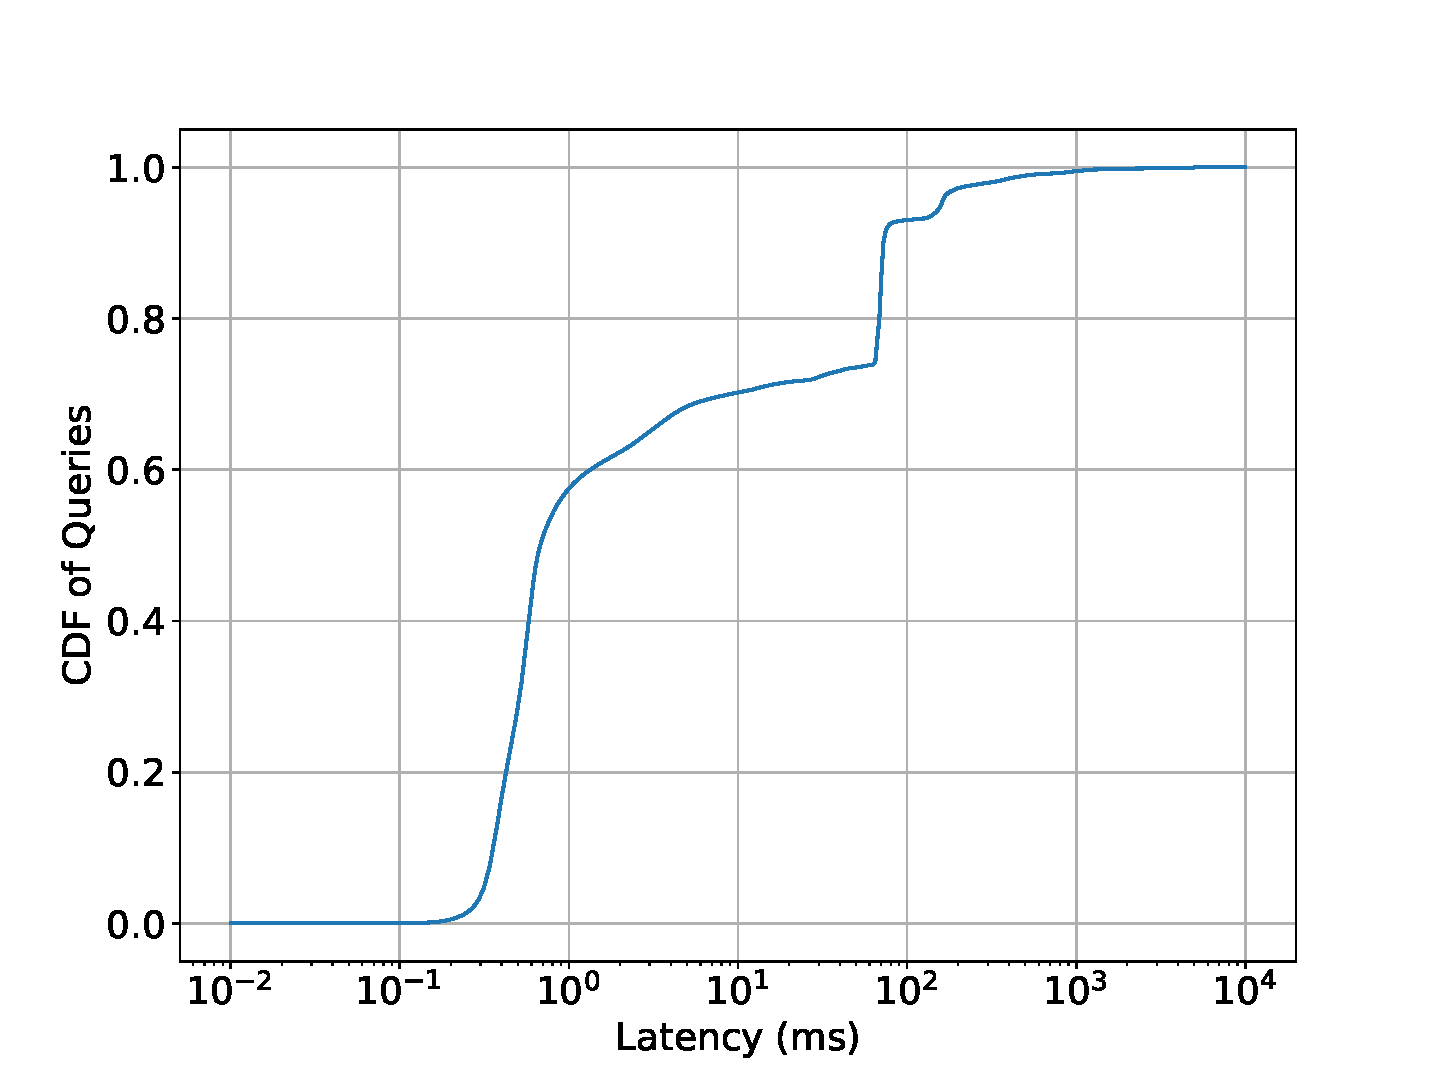
\includegraphics[width=\linewidth]{figures/all_dns_latencies_isi.pdf}
    \caption{CDF of user DNS query latencies seen at a recursive resolve at ISI, over the course of one year. Latencies are measured from the timestamp when the recursive resolver receives a client query to the timestamp when the recursive sends a response to that client query. The sub-millisecond latency for more than half of queries suggests most queries to this recursive are served by the local cache. }
    \label{fig:all_dns_latencies_isi}
\end{figure}

\begin{figure}
    \centering
    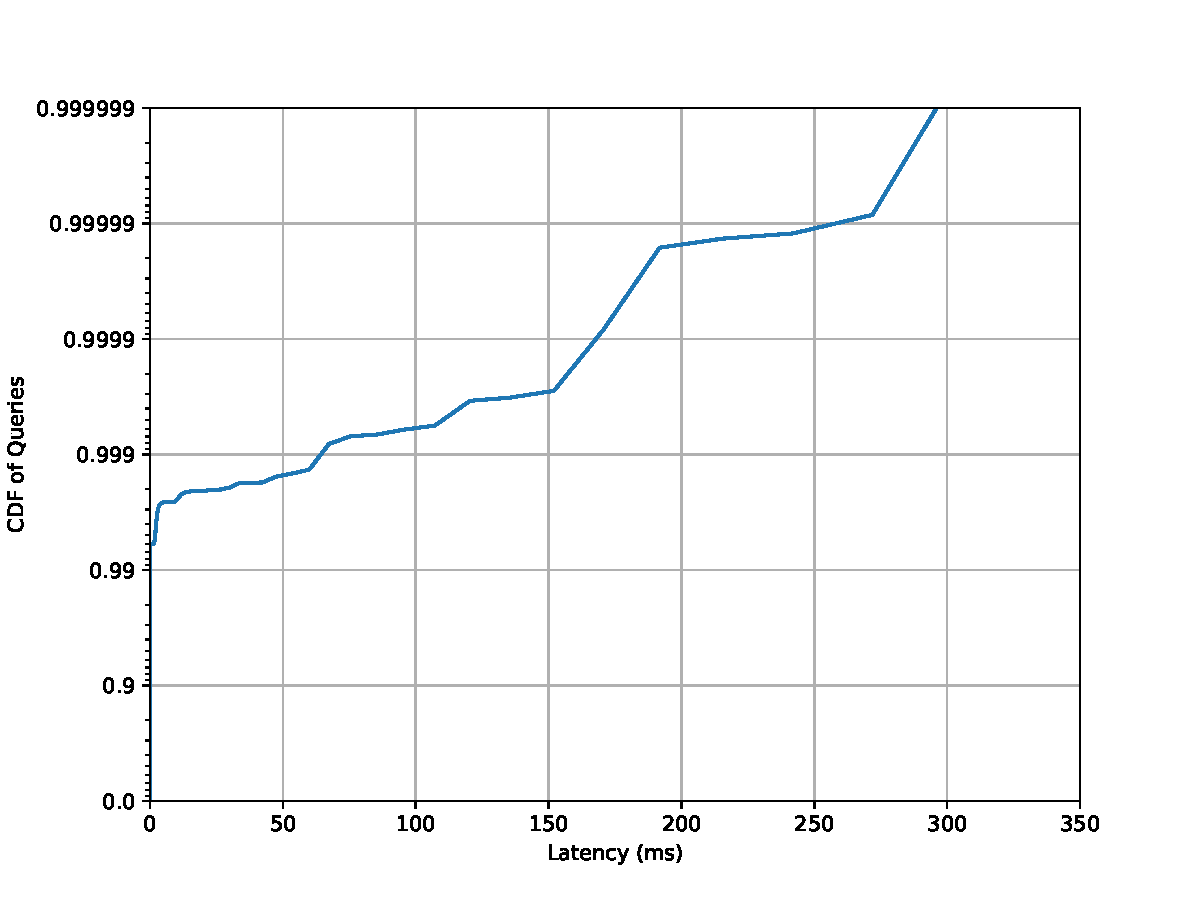
\includegraphics[width=\linewidth]{figures/isi_root_dns_latency.pdf}
    \caption{Root DNS latency for queries made by users of \ISItwo recursive resolver during 2018. This plot demonstrates the benefits of crowd-sourced caching and high TTLs of TLD records -- fewer than 1\% of queries generate a root request, and fewer than .1\% incur latencies greater than 100ms. User queries that did not generate a query to a root server were given a latency of 0. }
    \label{fig:isi_root_dns_latency}
\end{figure}

\section{Case Study: Redundant Root DNS
Queries}\label{case-study-redundant-root-dns-queries-1}

\label{ap:redundant_queries}

When we investigate the traffic from a recursive resolver to the root
servers in \Cref{sec:root_dns_latency}, we see as many as 900 queries to
the root server in a day for the COM NS record. Given the 2 day TTL of
this record, this query frequency is unexpectedly large. This large
frequency motivated us to analyze why these requests to roots occurred.
We consider a request to the root to be redundant if a query for the
same record occurred less than 1 TTL ago. Prior work has investigated
redundant requests to root servers as well, and our analysis can be
considered complementary since we discover different reasons for
redundant requests \cite{gao2014reexamining}.

To observe these redundant requests in a controlled environment, we
deploy a BIND instance (the resolver in \Cref{sec:root_dns_data_sources}
runs BIND v9.11.17) locally, and enable cache and recursion. We do not
actually look up the cache of the local BIND instance to see which
records are in it. Instead, we save the TTL of the record and the
timestamp at which we receive the record to know if the record is in
BIND's cache. We use BIND version 9.10.3 and 9.16.1. Because 9.16.1 is
one of the newest releases and 9.10.3 is a release from several years
ago, we can assume that pathological behavior is common in all versions
between these two releases. After deploying the instance, we simulate
user behavior by opening the top-1000 web pages according to GTmetrix
\cite{gtmetrix} using Selenium and headless Chrome, While loading web
pages, we collect network packets on port 53 using Tshark \cite{tshark}.

\begin{table}[]
\centering
\resizebox{\linewidth}{!}{%
\begin{tabular}{|l|l|l|l|l|l|l|}
\hline
\textbf{Step} & \textbf{\begin{tabular}[c]{@{}l@{}}Relative\\ Timestamp (second)\end{tabular}} & \textbf{From}         & \textbf{To}                    & \textbf{Query name} & \textbf{Query type} & \textbf{Response}                                                                                                                              \\ \hline
1             & 0.00000                              & client                & localhost                      & bidder.criteo.com   & A                   &                                                                                                                                                \\ \hline
2             & 0.01589                              & localhost             & 192.42.93.30 (g.gtld)          & bidder.criteo.com   & A                   &                                                                                                                                                \\ \hline
3             & 0.02366                              & 192.42.93.30 (g.gtld) & localhost                      & bidder.criteo.com   & A                   & \begin{tabular}[c]{@{}l@{}}ns23.criteo.com ns22.criteo.com \\ ns25.criteo.com ns26.criteo.com \\ ns27.criteo.com ns28.criteo.com.\end{tabular} \\ \hline
4             & 0.02387                              & localhost             & 74.119.119.1 (ns25.criteo.com) & bidder.criteo.com   & A                   &                                                                                                                                                \\ \hline
5             & 0.82473                              & localhost             & 182.161.73.4 (ns28.criteo.com) & bidder.criteo.com   & A                   &                                                                                                                                                \\ \hline
6             & 0.82555                              & localhost             & 192.58.128.30 (j.root)         & ns22.criteo.com     & AAAA                &                                                                                                                                                \\ \hline
7             & 0.82563                              & localhost             & 192.58.128.30 (j.root)         & ns23.criteo.com     & AAAA                &                                                                                                                                                \\ \hline
8             & 0.82577                              & localhost             & 192.58.128.30 (j.root)         & ns27.criteo.com     & AAAA                &                                                                                                                                                \\ \hline
9             & 0.82584                              & localhost             & 192.58.128.30 (j.root)         & ns25.criteo.com     & AAAA                &                                                                                                                                                \\ \hline
10            & 0.82592                              & localhost             & 192.58.128.30 (j.root)         & ns26.criteo.com     & AAAA                &                                                                                                                                                \\ \hline
11            & 0.82620                              & localhost             & 192.58.128.30 (j.root)         & ns28.criteo.com     & AAAA                &                                                                                                                                                \\ \hline
\end{tabular}%
}
\caption{Pattern example of the redundant root DNS requests. The last 5 requests to J root are redundant which may be caused by an unanswered request in step 4.}
\label{tab:redundant_example}
\end{table}

For these page loads, we observe 69215 DNS A \& AAAA-type requests
generated by the recursive resolver. 3137 of these requests are sent to
root servers and 2950 of them are redundant. Over 70\% of redundant
requests are AAAA-type. After investigating the cause of these redundant
queries, we find over 90\% of these redundant requests follow a similar
pattern. This pattern is illustrated by the example in
\Cref{tab:redundant_example}.

In \Cref{tab:redundant_example}, we show queries the recursive resolver
makes when a user queries for the A record of bidder.criteo.com. In step
1, the recursive resolver receives a DNS query from a client. According
to TTL heuristics, the COM A record is in the cache. In step 3, the TLD
server responds with records of authoritative nameservers for
``criteo.com''. Then, the recursive chooses one of them to issue the
following request to. However, for some reason (e.g.~packet loss), the
recursive resolver doesn't get a response from the nameserver in step 4.
Hence, the resolver uses another nameserver in step 5, which it learned
in step 3. At the same time, as seen in step 6 to 11, the recursive
sends (redundant) DNS requests to root servers, querying the AAAA-type
records for these nameservers. These requests are redundant since the
AAAA record for COM was received less than two days ago.

From the pattern demonstrated in \Cref{tab:redundant_example}, we
hypothesize that redundant requests to the root servers will be
generated for certain records when the following conditions are met.

\begin{enumerate}
        \item{A query from the recursive resolver to an authoritative nameserver times-out.}
        \item{The record queried for by the resolver to the root DNS server was not included in the 'Additional Records' section of the TLD's response.}
\end{enumerate}

The second condition is also why we were seeing more AAAA-type redundant
requests, because usually there are more A-type records in the
`Additional Records' section than AAAA-type records.

To see how much traffic is caused by our hypothesis in a real scenario,
we analyze packet captures on a recursive resolver (BIND 9.11.17)
serving users at \ISIone. To keep consistent with the other analysis we
do on this data set (\cref{sec:root_dns_latency}), we use packet
captures from 2018. 79.8\% of requests to roots are redundant and in the
pattern we described. The other 20.2\% consists of necessary requests,
and requests for which we have no hypothesis as to how they were
generated. We contacted developers at BIND, who said this may be a bug.

Now we know that a large number of unnecessary DNS requests to the roots
are redundant and are generated in BIND v9.16.1 and v9.10.3. Software
behaviors like the one described here can lead to orders of magnitude
more root DNS requests than would be necessary if recursives queried for
the record once per TTL. As demonstrated in
\Cref{fig:user_root_latency_per_day}, focusing on reducing the number of
these queries could both improve user experience, and reduce load on the
root server.

\section{Anycast CDN Performance
Visualization}\label{anycast-cdn-performance-visualization}

\label{ap:anycast_cdn_performance_viz}

In \Cref{sec:bg_cdn_anycast} we show the rings of a large anycast CDN,
and how users are distributed with respect to those rings. This
visualization does not include any information about latency, so we
provide one here. In \Cref{fig:microsoft_performance_deployment_map} we
show \feplural in R110, and associated performance users see to R110 in
each region. Transparent circles represent user populations, and their
radii are proportional to the user population. Population circles are
colored according to average median latency users in the metro see to
R110 -- red indicates higher latency while green indicates lower
latency. Latency generally gets lower, the closer users are to a \fe.
The CDN has focused on deploying \feplural near large user populations,
which has driven latencies quite low for nearly all users.

\begin{figure}
    \centering
    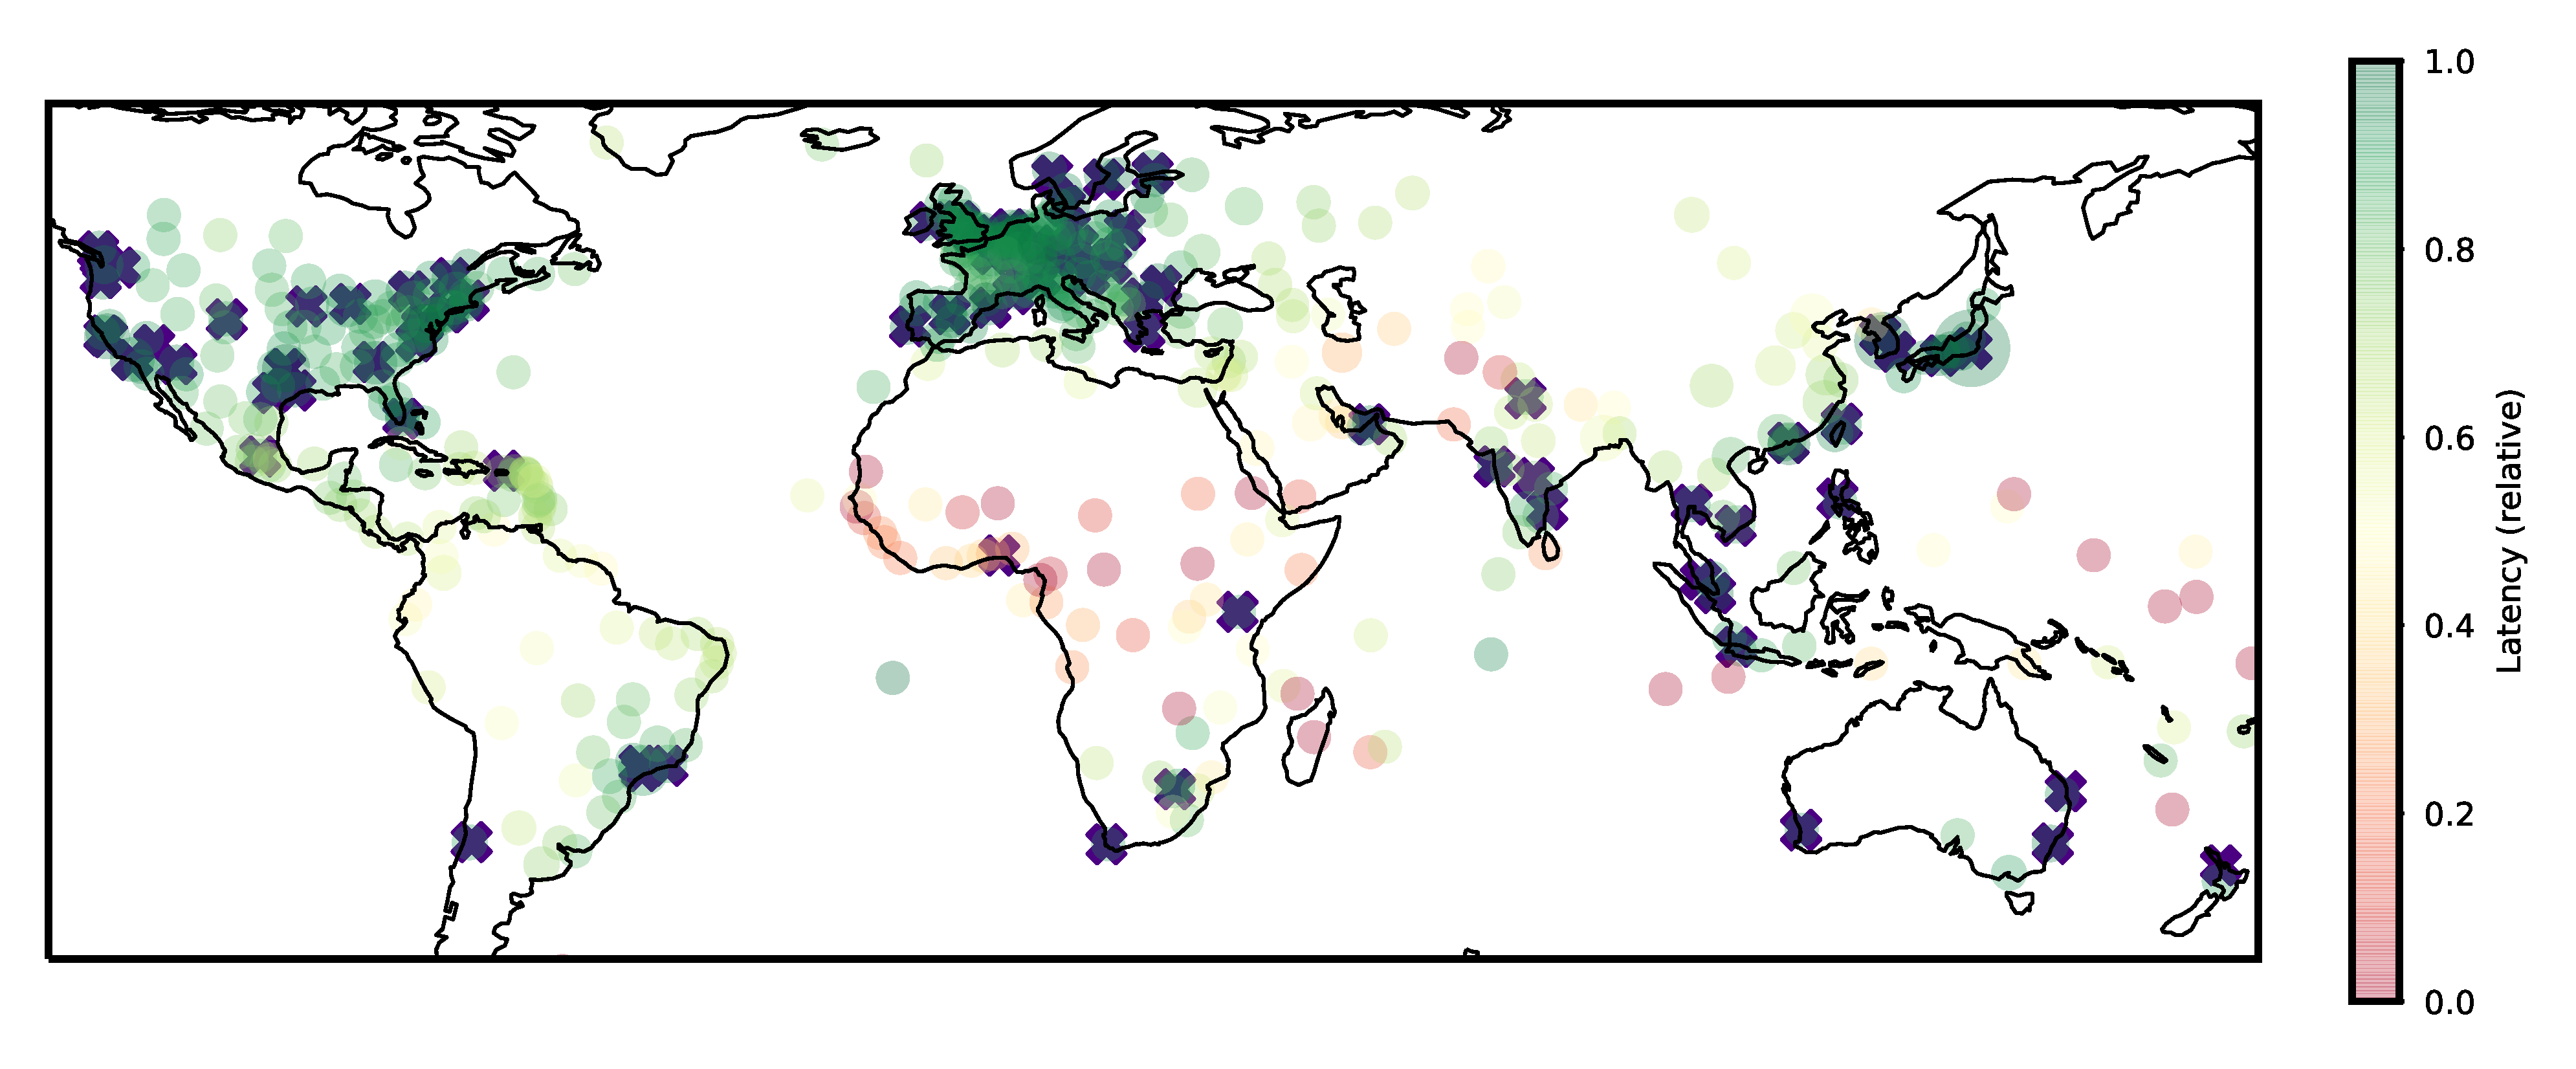
\includegraphics[width=\linewidth]{figures/microsoft_performance_deployment_map.pdf}
    \caption{A visualization of front-ends in R110 (purple Xs), and user populations (transparent circles). User populations are colored according to the relative latency they see, and have size proportional to user population. Red corresponds to high latency and green corresponds to low latency. Latency generally gets lower, the closer users are to a \fe, and \feplural are concentrated around large user populations.}
    \label{fig:microsoft_performance_deployment_map}
\end{figure}

\section{Supplementary Analysis of Routing
Efficiency}\label{supplementary-analysis-of-routing-efficiency}

\label{ap:distance_ranks}

As a way of measuring how efficient the root DNS and CDN route users to
queries, and how efficiency changes among root letters and rings, we
show how users are routed to sites. \Cref{sec:root_dns_anycast} and
\Cref{sec:cdn_anycast} show that path inflation either does not matter
to users, or is trumped by performance improvements from more sites. So,
looking at inefficiency is interesting but does not fully describe how
anycast performance affects users.

The cumulative histogram in \Cref{fig:distance_rank_root_dns} provides
us with a measure of the inefficiency that accumulates when adding more
anycast sites. In \Cref{fig:distance_rank_root_dns}, the bar for root
\(\mathnormal{j}\) and rank \(\mathnormal{i}\) measures the number of
users hitting no further than the \(\mathnormal{i}^{th}\) closest site
in deployment \(\mathnormal{j}\). For the purposes of calculation, if
\(\mathnormal{N_{R}}\) users use recursive resolver R, and
\(\mathnormal{q^j_i(R)}\) is the fraction of queries from recursive
resolver R hitting no further than the \(\mathnormal{i}^{th}\) closest
site in root deployment j to that recursive, we accumulate
\(\mathnormal{N_{R} q^j_i}\) users to rank index \(\mathnormal{i}\) for
root deployment \(\mathnormal{j}\) (\ie for the purposes of weighting).

\begin{figure}
    \centering
    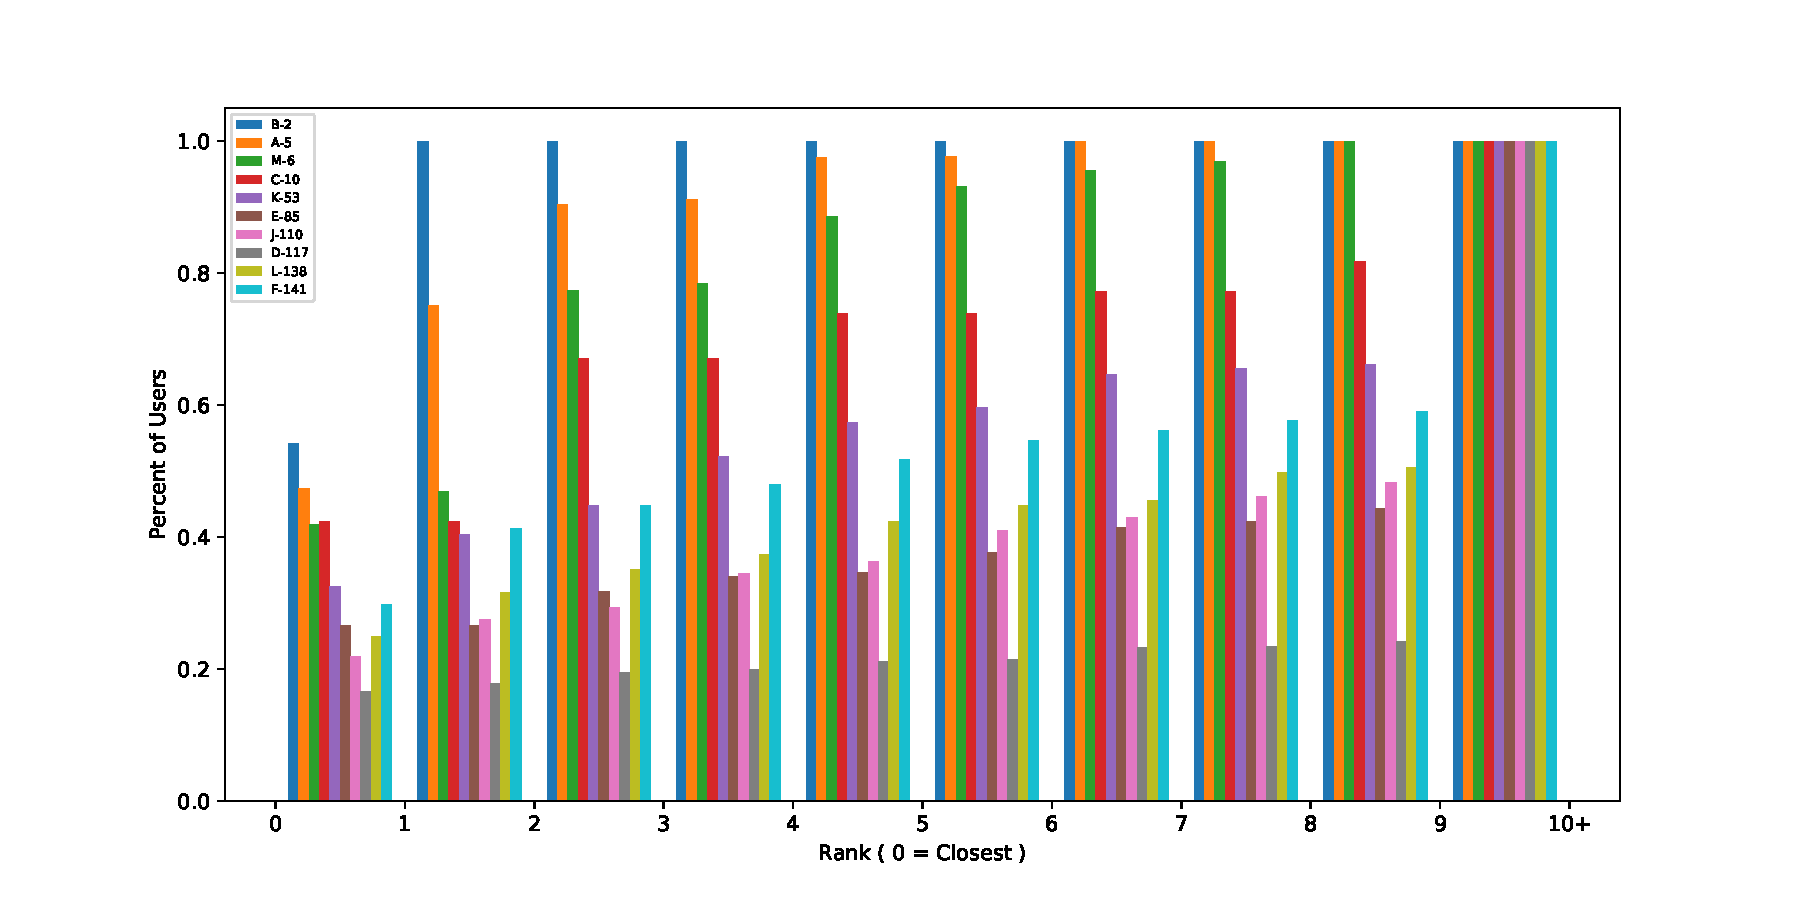
\includegraphics[width=\linewidth]{figures/distance_rank_root_dns.pdf}
    \caption{A cumulative histogram showing whether users tend to hit the closest available site for each root deployment. Root letters in the legend are listed according to their deployment sizes at the time, from smallest to largest. Generally, with increasing deployment size, there is an increase in "inefficiency" -- fewer users hit closer sites. }
    \label{fig:distance_rank_root_dns}
\end{figure}

One might expect that as the number of anycast sites increases, the
likelihood that a user hits the closest site decreases, and
\Cref{fig:distance_rank_root_dns} roughly demonstrates this trend.
However, there are noticeable exceptions to this rule -- roughly twice
as many users reach the closest or second-closest site when querying F
root compared to when querying D root, despite the fact that F root has
30 more anycast sites. Exceptions to the trend shows the success of some
root anycast operators at identifying and correcting anycast routing
problems \cite{Bellis15a}.

\begin{figure}
    \centering
    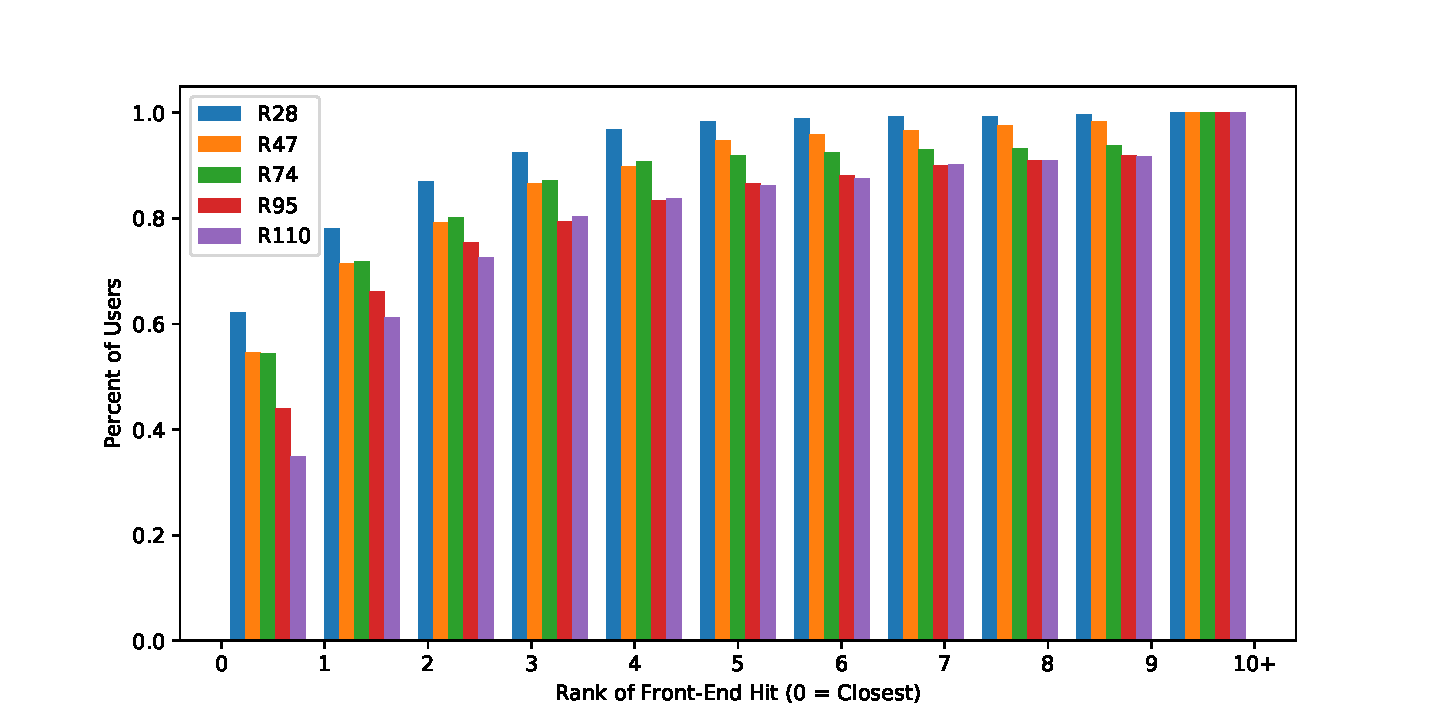
\includegraphics[width=\linewidth]{figures/distance_rank_microsoft.pdf}
    \caption{A cumulative histogram showing whether users tend to hit the closest available site for each ring. With increasing deployment size, there is an increase in "inefficiency" -- fewer users hit closer sites.}
    \label{fig:distance_rank_microsoft}
\end{figure}

As a comparison to \Cref{fig:distance_rank_root_dns} in
\Cref{fig:distance_rank_microsoft} we show how ``inefficient'' each ring
is. As in the root DNS, as deployment size increases, fewer users go to
their closest sites (as more relatively close competitor sites are
deployed) and inefficiency increases. In the root DNS, this inefficiency
was inconsequential because users rarely queried the roots. For the
anycast CDN, users do interact with the anycast CDN quite a lot (as
shown in \Cref{sec:anycast_cdn_latency}); however, as demonstrated in
\Cref{fig:microsoft_latency_benefit_increasing_ring} it is possible to
limit the impact of this inefficiency on users.

\iffalse
Don't remove this iffalse

% Do don't know why, but the pandocs pipeline started to include
% google docs comments at the end of the body.  So to fix that
% problem, the google doc requires an \iffalse as the last statement,
% then the following \fi will stop that comment block, effectively
% removing the comments from the final PDF.
\fi

\end{document}

